%%%%%%%%%%%%%%%%%%%%%%%%%%%%%%%%%%%%%%%%%
% OIST Doctoral Thesis - Final bound version
% LaTeX Template
% Version 0.2 (2016/04/06)
%
% This version is the final binding version which will be published.
%
% Original author:
% Jeremie Gillet
%
%%%%%%%%%%%%%%%%%%%%%%%%%%%%%%%%%%%%%%%%%

%-------------------------------------------------------------------------------
%	PACKAGES AND OTHER DOCUMENT CONFIGURATIONS
%-------------------------------------------------------------------------------

\documentclass[12pt, twoside]{book} % 12 pt font, two-sided book style
\usepackage[a4paper, includehead, headheight=0.6cm, inner=3cm ,outer=2.5cm, top=2.5 cm, bottom=2.5cm]{geometry}  % Changing size of document
\usepackage[english]{babel} % The document is in English
\usepackage[utf8]{inputenc} % UTF8 encoding
\usepackage[T1]{fontenc} % Font encoding
\usepackage{braket}

\usepackage{graphicx} % For including images
\graphicspath{{./Images/}} % Specifies the directory where pictures are stored

\usepackage{longtable} % tables that can span several pages
\usepackage[bf]{caption} % caption: FIG in bold
\usepackage{fancyhdr} % For the headers

\newcommand{\numberedchapter}{ % Preparation for numbered chapters
	\cleardoublepage % To make sure the previous headers are passed
	\fancyhead[RE]{{\bfseries \leftmark}}% Headers for left pages
	\fancyhead[LO]{{\bfseries \rightmark}}}% Headers for right pages
\newcommand{\unnumberedchapter}[1]{ % Preparation for unnumbered chapters
	\cleardoublepage % To make sure the previous headers are passed
	\phantomsection % To help hyperref link to the right page
	\addcontentsline{toc}{chapter}{#1} % Also adds the chapter name to the Contents
	\fancyhead[RE]{{\bfseries #1}} % Headers for left pages
	\fancyhead[LO]{}}%Headers for right pages

\usepackage{emptypage} % No headers on an empty page

\usepackage{eso-pic} % For the background picture on the title page
\newcommand\BackgroundPic{%
\put(-250,-140){%
\parbox[b][\paperheight]{\paperwidth}{%
\vfill
\centering
\includegraphics[width=\paperwidth]{symbol.jpg}%
\vfill
}}}

\usepackage{hyperref} % Adds clickable links at references

%-------------------------------------------------------------------------------
%	CUSTOM VALUES, COMMANDS AND PACKAGES (NOT IN THIS FILE)
%-------------------------------------------------------------------------------

% Open Preamble/mydefinitions.tex and enter some values (name, thesis title...)
% also include your own custom LaTeX functions and packages
% DO NOT add your packages here to ensure the temporary and final thesis use the same packages

%-------------------------------------------------------------------------------
%	VALUES FOR THE THESIS
%-------------------------------------------------------------------------------

\newcommand{\name}{James Schloss} % Author name
\newcommand{\thesistitle}{Advanced split-operator techniques for simulating quantum systems} % Title of the thesis
\newcommand{\submissiondate}{July, 2019} % Submission date "Month, year"
\newcommand{\supervisor}{Thomas Busch} % Supervisor name
%\newcommand{\cosupervisor}{C.~O'Supervisor} % Co-Supervisor name, comment this line if there is none


%-------------------------------------------------------------------------------
%	BIBLIOGRAPHY STYLE (pick the style you want)
%-------------------------------------------------------------------------------

\usepackage[square, numbers, sort&compress]{natbib} % for bibliography - Square brackets, citing references with numbers, citations sorted by appearance in the text and compressed (as in [4-7])
%\usepackage[longnamesfirst,round]{natbib} % Natural Sciences bibliography

%\bibliographystyle{Preamble/physics_bibstyle} % You may use a different style adapted to your field
\bibliographystyle{abbrvnat} % You may use a different style adapted to your field


%-------------------------------------------------------------------------------
%	YOUR PACKAGES (be careful of package interaction)
%-------------------------------------------------------------------------------

\usepackage{amsthm,amsmath,amssymb,amsfonts,bbm}% Math symbols

%-------------------------------------------------------------------------------
%	YOUR DEFINITIONS AND COMMANDS
%-------------------------------------------------------------------------------

% New Commands
\newcommand{\bea}{\begin{eqnarray}} % Shortcut for equation arrays
\newcommand{\eea}{\end{eqnarray}}
\newcommand{\e}[1]{\times 10^{#1}}  % Powers of 10 notation

% Defining a theorem box for Criteria
\newtheorem{critere}{Criterion}
\newcommand{\crit}[2]{
\begin{center}  
\fbox{ \begin{minipage}[c]{0.9 \textwidth}
\begin{critere}
\textbf{\textup{ #1}} --- #2
\end{critere}
\end{minipage}  } \end{center}
}

\newcommand{\jrs}[1]{\textcolor{magenta}{[#1]}}


\begin{document}

%-------------------------------------------------------------------------------
%	TITLE PAGE
%-------------------------------------------------------------------------------

\pagestyle{empty} % No page numbers
\frontmatter % Use roman page numbering style (i, ii, iii, iv...) for the preamble pages

\begin{titlepage}
\AddToShipoutPicture*{\BackgroundPic}
\begin{center}
\vfill
{\large \scshape Okinawa Institute of Science and Technology\\Graduate University}\\[0.7cm]
{\large Thesis submitted for the degree }\\[0.7cm]
{\Large Doctor of Philosophy}\\[0.5cm]
\rule{\textwidth}{1.5pt}\\[0.5cm]
{\huge \bfseries \thesistitle}\\[0.5cm]
\rule{\textwidth}{1.5pt}\\[2.5cm]
\hfill  by\\[1cm]
\hfill  {\large \bfseries\name}\\
\vfill
{\hfill \large Supervisor: \textbf{\supervisor}} \\
\ifx\cosupervisor\undefined\else{\hfill \large Co-Supervisor: \textbf{\cosupervisor}} \\ \fi
\vspace{1cm}
\hfill  \submissiondate
\end{center}
\end{titlepage}

%-------------------------------------------------------------------------------
%	PREAMBLE PAGES (comment out unnecessary pages)
%-------------------------------------------------------------------------------

\pagestyle{fancy} % Changes the headers
\renewcommand{\chaptermark}[1]{ \markboth{#1}{}} % Getting the chapter name right
\renewcommand{\sectionmark}[1]{\markright{\thesection\; #1}} % Getting the section name right
\fancyhf{}% Clears header and footer
\fancyhead[RO,LE]{\thepage} % page number on the outside of headers

\unnumberedchapter{Declaration of Original and Sole Authorship} 
\chapter*{Declaration of Original and Sole Authorship} 

I, \name, declare that this thesis entitled \emph{\thesistitle} and the data presented in it are original and my own work. 


I confirm that:
\begin{itemize}
\item No part of this work has previously been submitted for a degree at this or any other university.
\item References to the work of others have been clearly acknowledged. Quotations from the work of others have been clearly indicated, and attributed to them.
\item In cases where others have contributed to part of this work, such contribution has been clearly acknowledged and distinguished from my own work.
\item None of this work has been previously published elsewhere, with the exception of the following: 
\begin{itemize}
\item Chapter~\ref{ch:1d} is largely derived from a paper published in the New Journal of Physics (\textbf{18}(3):035012, 2016)~\cite{schloss2016}.
\item Chapter~\ref{ch:2d} is largely derived from a paper published in Phys. Rev. Fluids (\textbf{4}(5):054701, 2019)~\cite{zhang2019}.
\item The GPUE codebase, which is a primary topic in Chapter~\ref{ch:gpu} has been published in the Journal of Open Source Software (\textbf{3}(32):1037, 2018)~\cite{schloss2018}.
\item Chapter~\ref{ch:vortex_states} is largely derived from a recently submitted manuscript to Phys. Rev. Fluids (arXiv:1910.02364)~\cite{schloss2019}.
In addition, many figures for this chapter have been created for the GPUE documentation~\cite{docs}.
\item Figure~\ref{fig:bench} was created by Peter Wittek when comparing different numerical solvers~\cite{wittek2016}.
\item Figure~\ref{fig:expr_tree} was largely derived from tikz code provided by Xadisten during a Twitch livestream.
\item Figure~\ref{fig:coalesce} was largely derived from tikz code created by user Realz Slaw on stackexchange~\cite{stackoverflow}.
\item Figure~\ref{fig:mode_plot} was Reproduced by Nieddu \textit{et al.} and Kumar \textit{et al.}~\cite{Nieddu2016, kumar2015}.
\end{itemize}
All of the articles mentioned above have been (or will be published) under Creative Commons BY with attribution to the original authors, and in each chapter, I clearly define my focus in each publication.
\end{itemize}

Date:  \submissiondate

Signature: 





\unnumberedchapter{Abstract} 
\chapter*{Abstract} 
\subsection*{\thesistitle}

The split-step Fourier method is a powerful technique for solving partial differential equations and simulating quantum systems of various forms. In this body of work, we focus on several variations of this method to allow for simulations of one, two, and three-dimensional quantum systems, along with several notable methods for controlling quantum systems, including quantum optimal control and shortcuts to adiabaticity. We also examine the creation of stable, three-dimensional vortex structures in Bose--Einstein condensates through rotation, artificial magnetic fields, and phase imprinting, and we analyze chaotic vortex trajectories in two dimensions. In addition, we discuss algorithmic optimizations for implementing the compressed split-step Fourier method for graphics processing units and multicomponent simulations. All features present in this work have been incorporated into a state-of-the-art and open-source software suite known as GPUE and are justified with physical systems where such techniques have been applied.

\unnumberedchapter{Acknowledgment} 
\chapter*{Acknowledgment}

Firstly, I would like to acknowledge the work of my advisor, Thomas Busch.
His tireless effort to help his students pursue their best interests is honestly inspiring.
I greatly appreciate his kindness, honesty, and willingness to try new things.
I would also like to acknowledge the work of my online community, the Algorithm Archivists, as they constantly motivated me to learn new methods for my research.
This work has been supported by the Okinawa Institute of Science and Technology (OIST) Graduate University and used the computing resources of the Scientific Computing and Data Analysis section.
This work has also been supported by JSPS KAKENHI JP17J01488.
I would also like to thank (in no particular order) Lee, Mossy, Angela, Albert, J\'er\'emie, Peter, Irina, Ben, Tiantian, Peter (2), Rashi, Valentin, Ankur, the Quantum Systems Unit, and the OIST community for being such wonderful people and helping to varying degrees throughout my time at OIST.
Finally, I would like to thank Ayaka for helping me focus on something other than work for a change.

%\chapter{Copyright notice}

Unless otherwise stated, all figures shown in this work have either been created for the purposes of this thesis or designed and published as Creative Commons BY, with attribution to the original authors.

In particular,
\begin{itemize}
\item Chapter~\ref{ch:1d} is largely derived from a paper published in the New Journal of Physics (\textbf{18}(3):035012, 2016)~\cite{schloss2016}.
\item Chapter~\ref{ch:2d} is largely derived from a paper published in Phys. Rev. Fluids (\textbf{4}(5):054701, 2019)~\cite{zhang2019}.
\item Chapter~\ref{ch:vortex_states} is largely derived from a recently submitted manuscript to Phys. Rev. Fluids (arXiv:1910.02364)~\cite{schloss2019}.
\item The GPUE codebase, which is a primary topic in Chapter~\ref{ch:gpu} has been published in the Journal of Open Source Software (\textbf{3}(32):1037, 2018)~\cite{schloss2018}. In addition, many figures for this chapter have been created for the GPUE documentation~\cite{docs}.
\end{itemize}

In addition, Figure~\ref{fig:expr_tree} was largely derived from code provided by Xadisten during a Twitch livestream.


%\input{Preamble/abbreviations}
%\input{Preamble/glossary}
%\input{Preamble/nomenclature}
%\input{Preamble/dedication}

%-------------------------------------------------------------------------------
%	LIST OF CONTENTS/FIGURES/TABLES
%-------------------------------------------------------------------------------

\unnumberedchapter{Contents}
\tableofcontents % Write out the Table of Contents
%\unnumberedchapter{List of Figures}
%\listoffigures % Write out the List of Figures
%\unnumberedchapter{List of Tables}
\listoftables % Write out the List of Tables

%-------------------------------------------------------------------------------
%	THESIS MAIN TEXT - CHAPTERS
%-------------------------------------------------------------------------------

\addtocontents{toc}{\vspace{2em}} % Add a gap in the Contents, for aesthetics
\mainmatter % Begin numeric (1,2,3...) page numbering

\unnumberedchapter{Introduction} % Title of the unnumbered chapter
\section*{Introduction}
The Split-Step Fourier Method (SSFM) is an essential technique for simulating a variety of physical systems and is particularly useful for simulating the propagation of wave packets for single and multimode fibers~\cite{agrawal2000, sinkin2003, meirelles2005, min2003} and various quantum systems~\cite{bayindir2015, weideman1986, wang2005}, including all simulations performed in this work.
Though other methods, such as explicit and implicit Euler~\cite{butcher2016}, Crank-Nicholson~\cite{crank1947}, and Runge-Kutta~\cite{butcher2016}, can solve similar differential equations, the SSFM has distinct advantages over these methods.
For example, the SSFM is often much easier to parallelize than Runge-Kutta~\cite{brehler2017}, as it primarily relies on embarrassingly parallel element-wise matrix multiplications and Fast Fourier Transform (FFT) routines that have been optimized for parallel and distributed systems.
The SSFM also provides a lower error bound than either the Euler or Crank-Nicholson methods, and does not require implicit or tridiagonal solver \cite{conte2017, thomas1949} which are also not easily parallelizable~\cite{goddeke2010, wang1981, sweet1977}.
A full discussion of the advantages and disadvantages of the SSFM can be found in Chapter~\ref{ch:splitop}.

For the purposes of this text, we will be focusing on the application of the SSFM to quantum systems and will use primarily physical arguments to understand the details of the method, itself.
We will also discuss several numerical techniques for optimally simulating quanum systems on massively parallel Graphics Processing Units (GPUs), along with software developed for this purpose: GPUE, the Graphics Processing Unit Gross-Pitaevskii Equation Solver.
This work will discuss several additional areas of interest for implementing similar solvers on GPUs, including distributed transposes and important considerations for traditional FFT routines for simulating quantum systems on multiple GPU devices.

As such, it is important to first discuss several principles of quantum systems in Chapter~\ref{ch:qs}, incuding the Schr\"odinger equation which governs the dynamics for simple quantum systems along with several notable variations that correspond to physical systems to be discussed in this work.
Further elaboration on advances in scientific computing, including the massively parallel Graphics Processing Unit (GPU) will be discussed in Chapter~\ref{ch:gpu}, and the SSFM method, along with variations on the method for vortex simulations will be discussed in Chapter~\ref{ch:splitop}.
In Chapter~\ref{ch:1d}, we will discuss the basics of quantum engineering, by generating macroscopic superposition states of highly-interacting quantum particles with quantum optimal control and shortcuts to adiabaticity.
In Chapter~\ref{ch:dynamics}, we will discuss specifically superfluid simulations and several notable methods for generating and controlling vortex structures both theoretically and experimentally, along with numerical hurdles with simulating such systems on GPU architecture, and in Chapter~\ref{ch:2d}, we will discuss an application of the GPUE codebase in the generation of chaotic vortex dynamics with a small number of vortices in a two-dimensional superfluid simulation.
In Chapter~\ref{ch:3d}, we will discuss challenges in simulating fully 3-dimensional, multi-component superfluid systems on GPU architecture, including dynamic field generation, storage limitations, and spectral methods to optimize the simulation, itself.
In Chapter~\ref{ch:vortex_states}, we will apply the numerical techniques introduced in this text to simulate a novel device that couples the evanescent field of an optical nanofiber to generate vortex ring-like structures in a toroidally trapped superfluid system.
Finally, we will conclude by discussing key results from this work, along with future directions in both theoretical and computational physics.
 % Introduction (unnumbered)

\numberedchapter % Regular chapters following

\chapter{Introduction to the split-operator method} \label{ch-splitop}


\chapter{Engineering NOON states in one-dimensional quantum gases}
\label{ch:1d}

Until recently, simulating dynamic control protocols to engineer specific quantum states have been difficult to perform on GPU devices without full control of the software, itself.
This meant that researchers wishing to engineer specific quantum states by using GPU simulations would be required to have domain-specific knowledge in both software design and quantum mechanics, neither of which are trivial to understand.
This chapter serves as motivation for several methods to be discussed in Chapter~\ref{ch:gpu} to allow for the simulation of quantum control methods on GPU devices, with a particular focus on quantum optimal control~\cite{werschnik2007} and Shortcuts To Adiabaticity (STA)~\cite{guery2019}.
Both of these control protocols will be used in a physical example for the non-adiabatic generation of superposition states in a one-dimensional Tonks--Girardeau (TG) gas~\cite{schloss2016}.
To start, I will discuss the field of optimization algorithms before moving to STA protocols and a physical system using both in practice.

The work in this chapter has been published in \textit{New Journal of Physics}~\cite{schloss2016}, and in this publication, I performed all calculations for all the figures generated and focused primarily on optimal control methods.
The STA protocol was devised by J\'er\'emie Gillet, and the research was supervised by Albert Benseny and Thomas Busch.

\section{Optimization methods}

Optimization algorithms have become essential to many areas of modern computing and focus on either minimizing or maximizing a cost function by modifying several control parameters~\cite{lewis2012}.
The number of control parameters create an $n$-dimensional space to traverse, and optimization algorithms are tasked at finding the global minimum or maximum of this domain.
For certain domains, it is difficult to find a global optimization strategy and many methods instead get caught in local minima while attempting to find the appropriate solution.
Because generalized optimization is such a fundamental problem, there are many known optimal control methods, such as gradient descent~\cite{ruder2016}, the Nelder--Mead or simplex method~\cite{nelder1965}, genetic algorithms~\cite{koza1997}, and many more~\cite{lewis2012}.
Of these, gradient descent is often considered to be one of the easiest to implement with favorable complexity and convergence guarantees, and because of this, it has become ubiquitous in many areas such as machine learning, which is of particular interest for GPU engineering. 
Even so, there are limitations to gradient descent, such as its dependence on calculating the gradient of the cost function's solution domain along with lengthy convergence times for high-precision solutions.

For this work, I am primarily interested in the area of quantum optimal control, which is a method typically used to determine the optimal time-dependent control parameters necessary to transform an initial state to a final, desired state~\cite{werschnik2007}.
This means that one will often be maximizing the fidelity between states, defined as $\mathcal{F} = |\braket{\psi|\phi}|^2$, where $\psi$ is the engineered quantum state and $\phi$ is the state one is attempting to replicate.
This problem can be re-framed as an attempt to find the maximum of a fidelity \textit{landscape}, where each point in the domain is a calculation of the fidelity.
This means that each point in the fidelity landscape necessarily involves solving the Schr\"odinger equation for chosen control parameters.
For this reason, I will be introducing a gradient-less (derivative-free) optimization algorithm, the Nelder--Mead (simplex) method, which is often used as a heuristic approach to this problem and there are several known optimizations for this method~\cite{nelder1965,kolda2003,lewis2007}.
The Nelder--Mead method is also the recommended optimization algorithm for the chosen quantum optimal control method of the physical example that will be discussed in Section~\ref{sec:CRAB}, Chopped RAndom Basis (CRAB) optimal control.

\subsection{Nelder--Mead}
\label{sec:NM}

The Nelder--Mead method is one of the most commonly implemented gradient-less optimization algorithms to-date and relies heavily on the concept of a simplex, which is a generalization of the three-dimensional tetrahedron to $n$-dimensions.
For example, a 0-simplex is a point, a 1-simplex is a line, a 2-simplex is a triangle, a 3-simplex is a tetrahedron, and so on.
If the Nelder--Mead method is attempting to optimize a cost function with $n$ control parameters, an $n+1$ point simplex will be created, and the points of this simplex will be manipulated until they have converged to a minimum or maximum in the domain.
For this section, I will focus on the method introduced in the original work by Nelder and Mead in 1965 while working at the National Vegetable Research Station in Warwick, England~\cite{nelder1965}.

For $P_i \in i=\{0,...,n\}$ simplex points with heights of $y_i \in i=\{0,...,n\}$, the Nelder--Mead method is tasked at minimizing all points such that $\sqrt{\sum(y_i-\bar y)^2/n} < \eta$, where $\bar y$ denotes the height of the centroid location of the simplex, and $\eta$ is some pre-defined convergence threshold value.
This convergence criteria assumes that if all points have converged with this method, the final location must be the minimum of the optimization domain; however, as mentioned in the previous section, this method may become trapped in a local minimum.
At every step in the Nelder--Mead method, the points with the highest and lowest values are determined and denoted as $P_h$ and $P_l$, respectively.
In addition, the centroid location is found as $\bar P$.
This method then performs up to three basic operations on the simplex, itself:

\begin{description}

\item[Reflection] For this operation, $P_h$ is flipped across $\bar P$, such that the new location,
\begin{equation}
P^* = (1+\alpha)\bar P - \alpha P_h.
\end{equation}
\noindent Here, $\alpha > 0$ is a constant known as the reflection coefficient.
After this operation, the new height is compared to $y_l$.
If it is lower, the method proceeds to an expansion step.
Otherwise, the method checks whether the new height is lower than some other $y_i \in \{0,...,n\},n\neq \{l,h\}$, and if it is, the point is kept and the method continues to find the new simplex ordering.
If it is found that the reflected point, $P^*$, is higher in value than all other points, the method then keeps whichever point corresponds to the lowest height between the reflected and previous highest point and proceeds to the contraction step.

\item[Expansion] For this operation, an expansion is performed, such that the new location,
\begin{equation}
P^{**} = \gamma P^* + (1-\gamma)\bar P.
\end{equation}
\noindent Here, $\gamma > 1$ is a constant known as the expansion coefficient.
If the new height is less than the previously lowest point, the expanded point, $P^{**}$, is kept, otherwise the reflected point is kept.

\item[Contraction] For this operation, a contraction is performed, such that the new location,
\begin{equation}
P^{**} = \beta P_h + (1-\beta)\bar P.
\end{equation}
\noindent Here, $0 < \beta < 1$ is a constant known as the contraction coefficient.
If the contracted point, $P^{**}$, is lower than the previous highest point, the contracted point is kept, otherwise, the entire simplex is contracted closer to the lowest point with $P_i = (P_i + P_l)/2$.
\end{description}

Each step in the Nelder--Mead method begins with a proposed reflection of the least optimal point about its centroid position.
From there, the method follows the protocol described above.
The choice of $\alpha$, $\beta$, and $\gamma$ is somewhat arbitrary and should be optimized by-hand.
An example of the centroid locations for minimization using this method with the Rosenbrock banana function~\cite{pohlheim2007} can be seen in Figure~\ref{fig:minimize_NM}.

\begin{figure}
\center 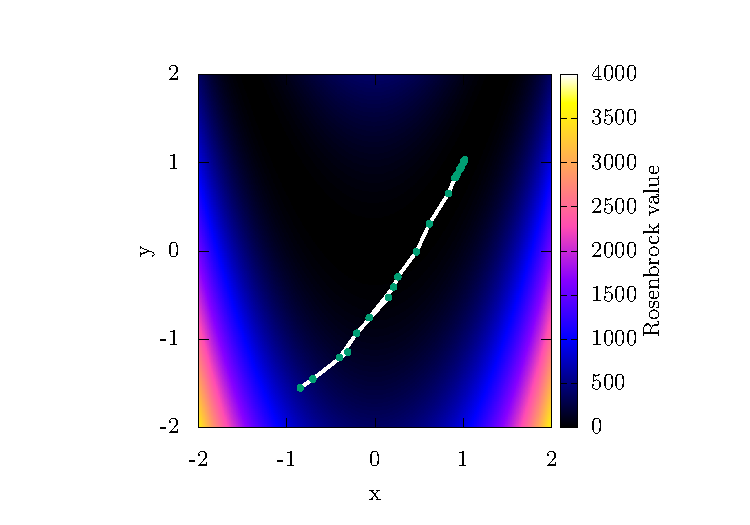
\includegraphics[width=0.75\textwidth]{data/1d/NM/NM.pdf}
\caption{Plot of the centroid locations (green dots connected with white line) for the Nelder--Mead method while optimizing the Rosenbrock banana function, $f(x,y)=(a-x)^2+b(y-x^2)^2$, with $a=1$ and $b=100$.
Here, centroid locations start at $(-0.851,-1.553)$ and end at the known minimum of $(1,1)$ in 19 iterations.
Here, $\alpha = 1$, $\beta = 0.5$, and $\gamma = 1.5$.}
\label{fig:minimize_NM}
\end{figure}

Even though the Nelder--Mead method is a heuristic approach and can become stuck in a local minimum, as long as a sufficient number of random simplexes are chosen at the start of the simulation, it can be used to find an adequately optimal solution.
Ultimately, any gradient-less optimization algorithm can be used to traverse the fidelity landscape for quantum optimal control, and in the next section, I will discuss a common method used in the field: the CRAB optimal control method.

\subsection{Chopped random basis optimal control}
\label{sec:CRAB}

The CRAB technique works by modifying a control parameter for a given system, $\Gamma$, with a multiplicative term as
\begin{equation}
\Gamma^{\text{CRAB}}(t) = \Gamma^0(t)\gamma(t),
\end{equation}

\noindent where $\Gamma^0(t)$ is an initial guess, and the function $\gamma(t)$ is written as a sum of $2J$ sinusoidal functions,
\begin{equation}
\gamma(t)=1+\frac{1}{\lambda(t)}\sum_{j=1}^J(A_j \sin(\nu_jt) + B_j\cos(\nu_jt)).
\end{equation}

\noindent Here, $\lambda(t)$ is usually defined by the system, such that $\Gamma^{\text{CRAB}}$ and $\Gamma^0$ coincide at initial and final times.
This means that $\lim_{t\rightarrow 0} \lambda(t) = \lim_{t\rightarrow T}\lambda(t) = \infty$, where $T$ is the final time of evolution.
As such, any smooth function may be chosen with these constraints.
For example, one might use
\begin{equation}
\lambda(t) = \frac{T^2}{4t(t-T)},
\end{equation}
\noindent which satisfies the provided conditions.
This then transforms the optimal control problem into an optimization of the space spanning $\{A_j, B_j, \nu_j\}$, which can be done by using Nelder--Mead with a simplex of random initial points.
As an example, if $J = 10$, a thirty-dimensional space would be created and a thirty-one simplex would be formed to traverse this space.
It is important to remember that each new simplex and simplex-operation requires re-solving the Schr\"odinger equation for those values, and as such, this is a computational costly technique.
Even though higher $J$ values will produce a more accurate result, lower values should be chosen, if possible.

This method is a general-purpose computational tool for determining the optimal pulse to ensure the generated state is as close to the desired state as possible, and I will show an example of it being used later in this chapter.
Even so, it is sometimes worthwhile to attempt to devise analytical frameworks that serve a similar purpose, and for certain systems, this can be done with STA protocols.

\section{Shortcuts to adiabaticity}

STA protocols are semi-analytical methods that allow for quantum state generation while retaining the effects of adiabatic movement.
Here, adiabatic processes are defined as actions by which slow changes in the control parameters leave particular properties invariant, such as the quantum number~\cite{guery2019}.
The ultimate goal of STA protocols is to achieve adiabatic motion in sub-adiabatic time, and this can be done in a number of ways; however, in this section, I will introduce only the invariant-based inverse-engineering approach using Lewis--Riesenfeld invariants~\cite{torrontegui2013}.
In particular, I will focus on the specific methods necessary for the example to be introduced later in this chapter and much of this section will follow traditional derivations from various sources~\cite{torrontegui2013,guery2019, schloss2016}.

With the method of Lewis-Riesenfeld invariants, the theory for relating different eigenstates of a time-dependent, Hermitian invariant to the solutions to the Schr\"odinger equation~\cite{lewis1969} can be applied to systems with time-dependent Hamiltonians, such that
\begin{equation}
i\hbar \frac{\partial I(t)}{\partial t} - \left[\mathcal{\hat H},I(t)\right] = 0,
\end{equation}
\noindent where $I(t)$ is the invariant.
This ensures that the expectation values for the states driven by $\mathcal{\hat H}$ are constant in time.
It is possible to expand the state of the system $\ket{\Psi(t)}$ into the orthonormal basis of the invariant with,
\begin{equation}
\ket{\Psi(t)} =\sum_{n=1}^\infty c_n e^{i\alpha_n(t)} \ket{\phi_n(t)},
\end{equation}
\noindent where $c_n$ are time-independent amplitudes for each state, and $\ket{\phi_n(t)}$ are orthonormal eigenvectors of the invariant, such that
\begin{equation}
I(t) = \sum_n^\infty\ket{\phi_n(t)}\lambda_n\bra{\phi_n(t)}.
\end{equation}
\noindent Here, the $\lambda_n$ are real constants, and the phase is defined as ~\cite{lewis1969}
\begin{equation}
\alpha_n(t) = \frac{1}{\hbar}\int_0^t\braket{\phi_n(t')|i\hbar\frac{\partial}{\partial t'} - \mathcal{\hat H}(t')|\phi_n(t')}dt'.
\end{equation}

From here, inverse engineering can be used to create the desired time-dependent Hamiltonian, by imposing some dynamics on the system.
The phases, $\alpha_n(t)$ may be chosen as arbitrary functions to create a time-dependent, unitary evolution operator,
\begin{equation}
U = \sum_n^\infty e^{i\alpha_n(t)}\ket{\phi_n(t)}\bra{\phi_n(0)},
\end{equation}
\noindent that obeys $i\hbar \dot U = \mathcal{\hat H}(t)U$ and the dot is a time-derivative.
If one considers Hamiltonians of the Lewis and Leach variety~\cite{lewis1982},
\begin{equation}
\mathcal{\hat H} = \frac{p^2}{2m}  -F(t)x + \frac{m}{2}\omega^2(t)x^2 + \frac{1}{\rho(t)^2}U\left[\frac{x-x_c}{\rho(t)}\right] + f(t),
\label{eqn:HSTA}
\end{equation}
there will be an invariant that is quadratic in momentum,
\begin{equation}
I = \frac{1}{2m}[\rho(p-m\dot x_c)-m\dot \rho(x-x_c)]2 + \frac{1}{2}m\omega_0^2\left( \frac{x-x_c}{\rho} \right)^2 + U\left( \frac{x-x_c}{\rho}\right).
\end{equation}
\noindent These equations are valid so long as $\rho$, $x_c$, $\omega$, and $F$ satisfy
\begin{align}
\ddot \rho + \omega^2(t)\rho &= \frac{\omega_0^2}{\rho^3} \label{eqn:rho}\\
\ddot x_c + \omega^2(t)x_c &= F(t)/m \label{eqn:xc},
\end{align}
\noindent with $\omega_0$ as a constant whose physical interpretation depends on the system.
As in the case of quantum optimal control, additional constraints must be considered to ensure the Hamiltonian and its invariant commute at initial and final times $t_0$ and $T$.

The obvious drawbacks to STA methods are the strengths of quantum optimal control.
Where shortcuts can only be used on a specific subset of problems to evolve adiabatically and that are amenable to the analytical methods used, quantum optimal control is a more general tool for a wider variety of systems.
On the other hand, STA protocols are semi-analytical and if such protocols can be found, they greatly reduce the computational cost to engineering particular quantum states.
Now that I have provided specific examples of methods used in quantum engineering, it is time to put them into practice with an example of creating large-scale superposition states non-adiabatically in the highly-correlated TG gas regime.

\section{Non-adiabatic generation of NOON states in a Tonks--Girardeau gas}

For this example application of quantum optimal control and STA protocols, I am interested in generating the maximally entangled $\ket{N,0} + \ket{0,N}$ (NOON) state, which is composed of two modes where all particles can be found exclusively in one or the other.
Recently, Hallwood \textit{et al.} proposed an experimentally realistic method to generate NOON states in a gas of strongly interacting, neutral bosons on a one-dimensional ring.
In this system, different rotational states can be coupled by breaking the rotational symmetry and it is possible to create superposition states with rotating and non-rotating components.
Because the atoms are considered to be in the strongly correlated TG gas regime, this process results in a macroscopically-entangled state.
It is worth discussing the TG gas in further detail before moving to the precise method of NOON state generation for this example.

\subsection{Tonks--Girardeau gas}

As mentioned in Chapter~\ref{ch:splitop}, the TG gas consists of a number of bosons that have the properties of spinless, non-interacting fermions.
This is a particular case of the one-dimensional Schr\"odinger equation where the repulsive interaction strength $g\rightarrow\infty$.
In this case, the bosons cannot be at the same location, which acts formally similar to the Pauli-exclusion principle for fermionic systems.
In this case, the bosonic Hamiltonian can be solved by the Bose--Fermi mapping theorem \cite{girardeau2001ground, girardeau2001measurement}, which replaces the interaction terms in the Hamiltonian with a boundary condition on the many-body bosonic wavefunction,
\begin{equation}
\Psi_B(x_1, x_2, \ldots, x_N) = 0,\qquad \mathrm{if}\qquad x_i - x_j = 0 \quad\textrm{with}\quad i \ne j,
\end{equation}

\noindent following the many-body Hamiltonian,
\begin{equation}
\mathcal{\hat H} = \sum_{n=1}^N\left(\frac{p_n^2}{2m} + V_n + b\delta(x_n)\right) + \sum_{j<k}V(|x_j - x_k|).
\end{equation}

\noindent Here, $p_n = -i\hbar\frac{\partial}{\partial x_n}$, $V_n = \frac{1}{2}m\omega^2x_n^2$, $b\delta(x_n)$ is a delta barrier with strength $b$, and $V$ is an interaction potential between bosonic particles.
This allows us to treat strongly interacting bosons as spinless, non-interacting fermions, for which the many-body wavefunction can be calculated using the Slater determinant~\cite{slater1929},
\begin{equation}
\Psi_F (x_1, x_2, \ldots, x_N) = \frac{1}{\sqrt{N}} \det\Big[\psi_n(x_j)\Big]_{n,j=1}^N,
\end{equation}
\noindent where $\psi_n(x_j)$ are the single-particle eigenstates of the trapping potential $V_n$.
Because the fermionic many-body wavefunction is anti-symmetric, it needs to be symmetrized for bosonic states as, 
\begin{equation}
\Psi_B(x_1, x_2, \ldots, x_N) =
\prod_{i < j}
\mathrm{sgn}(x_i - x_j)\Psi_F(x_1, x_2, \ldots, x_N),
\end{equation}
\noindent which means that calculating the time evolution of a TG gas requires evolving single-particle states, governed by a much simpler Hamiltonian.

\subsection{NOON states in a TG gas}
\label{sec:controltro}

Similar to other ring systems introduced in the literature~\cite{das2002,girardeau2009}, the system suggested by Hallwood \textit{et al.} considers a gas of $N$ interacting bosons of mass $m$ on a one-dimensional ring with circumference $L$~\cite{hallwood2010}.
In addition, this system includes a potential barrier, modeled by a Dirac $\delta$-function that rotates with an angular frequency $\Omega$, as shown in Figure~\ref{fig:ring_scheme}.
In the rotating frame, the scaled Hamiltonian of the system in the rotating frame is given by \cite{hallwood2010}
\begin{equation}H^{(N)} = \sum_{n=1} ^{N} \left[{\frac{1}{2}\bigg(-i\frac{\partial}{\partial x_n}-\Omega}\bigg)^2 + b\delta(x_n) +g \sum_{j<k} ^{N} \delta (x_j - x_k )\right],
\end{equation}
\noindent where $b$ is the height of the barrier (in units of $\hbar^2/mL^2$), $x_n \in \left[-1/2,1/2\right]$ is the position of the $n$--th particle (in units of $L$) and $g$ (in units of $\hbar^2/mL^2$) is the effective interaction strength between the atoms.
As discussed in the previous section, the evolution of the full TG gas can be calculated from the evolution of single-particle states, and in the case of this system, the Hamiltonian in the laboratory frame becomes,

\begin{equation}
H = -\frac{1}{2} \frac{\partial^2}{\partial x} + b\delta \left[ x-x_0(t) \right], 
\end{equation}
where $x_0$ is the position of the barrier at time $t$. 

\begin{figure}
\center 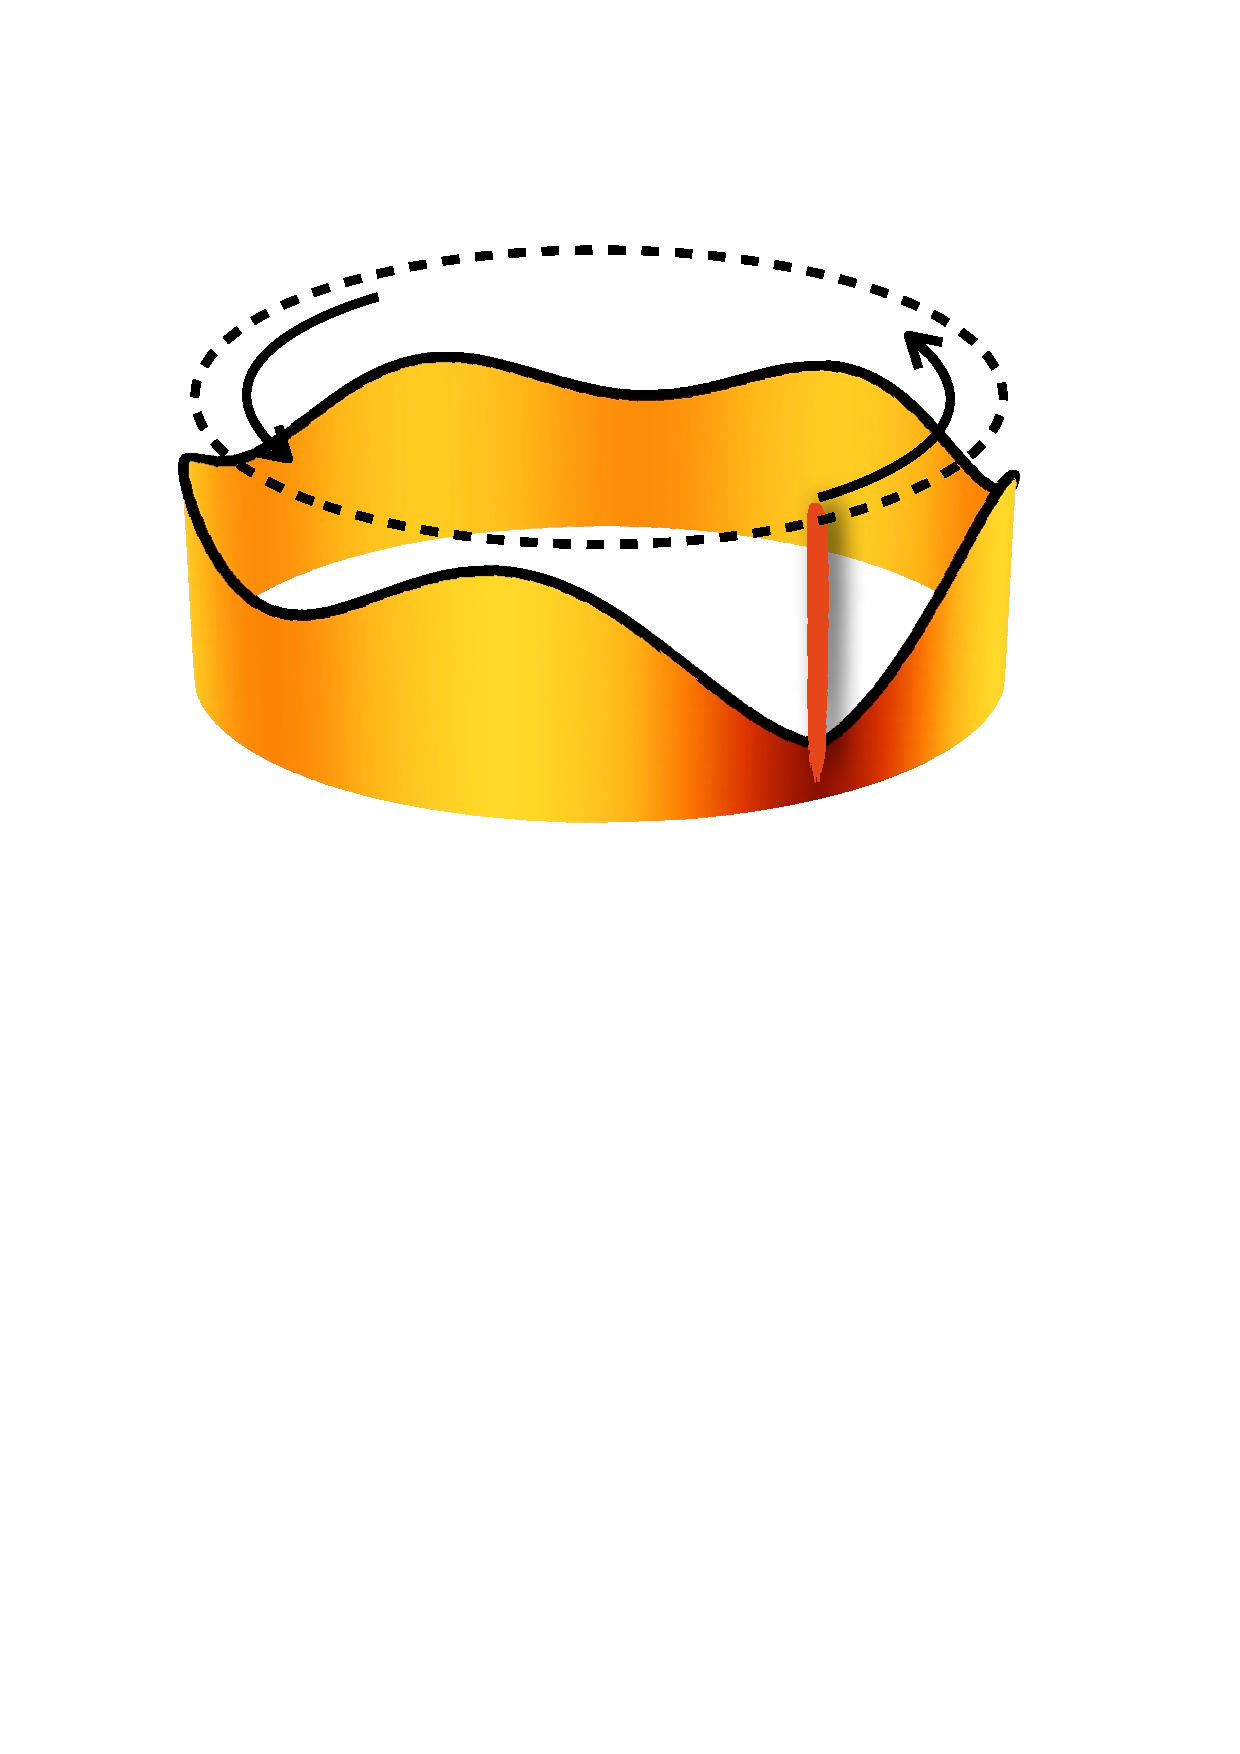
\includegraphics[width = 0.5\textwidth]{data/1d/scheme.pdf}
\caption{Schematic of the system.
Here, the density profile for five atoms in a TG gas is shown being stirred by a highly localized potential, indicated by the vertical line.}
\label{fig:ring_scheme}
\end{figure}

The energy spectrum of this system is shown in Figure~\ref{fig:avoid} as a function of the rotational frequency $\Omega \equiv \dot x_0 /L$ of the system.
In Figure~\ref{fig:avoid}(a) it is shown that in the absence of a barrier, when the eigenstates of $\mathcal{\hat H}$ are plane waves with quantized angular momentum in integer multiples of $2 \pi$, each angular momentum manifold exists separately such that the energy levels cross; however when $b>0$ (Figure~\ref{fig:avoid}(b)), the rotational symmetry is broken and avoided crossings appear in the energy spectrum.
This makes transitions between different manifolds possible~\cite{schenke2012}.

\begin{figure}

 \centering
 \subfigure{
 \centering
 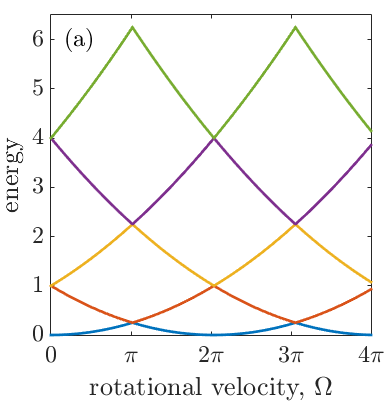
\includegraphics[width = 0.4\linewidth]{data/1d/cross.png}} 
 \subfigure{
 \centering
 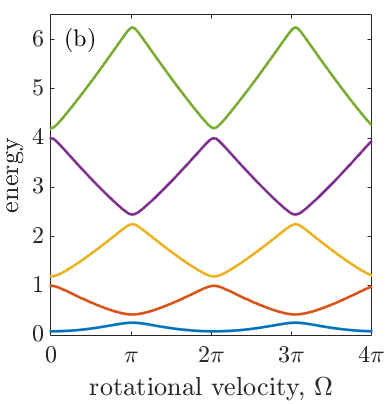
\includegraphics[width = 0.4\linewidth]{data/1d/nocross.png}}

\caption{Single-particle energy spectrum as a function of $\Omega$ for a barrier height of (a) $b = 0$ and (b) $b=2$.
When a barrier is present in the system, avoided crossings appear in the energy spectrum which grow as the barrier strength increases.}
\label{fig:avoid}
\end{figure}

By adiabatically accelerating the barrier's rotational frequency from 0 to $\pi$, a particle will enter a superposition between two rotational states, and in the case of the TG gas, this will create a macroscopic NOON superposition state between successive values of angular momentum~\cite{hallwood2010}.
This means that the manifolds will have an angular momentum of 0, 1, 2, $\ldots$, $N$, where $N$ is the number of particles in the system.
Any non-adiabatic behavior around the rotational frequencies of the avoided crossings can lead to a transition to a higher energy state and destroy the NOON state.
For this reason, the condition for adiabaticity must depend on the gap size, which is dictated by the barrier strength~\cite{nunnenkamp2008}; however, for a constant delta barrier, the gap size stays constant to first-order approximation~\cite{hallwood2007}.

Because this system requires adiabatic movement to properly generate the NOON state, it is difficult to efficiently generate it experimentally.
For this reason, it is a perfect example of a system where quantum optimal control and STA protocols can be used to rapidly engineer the appropriate states.
For quantum optimal control in this system, a non-adiabatic rotational frequency $\Omega(t)$ must be found, for which I will use the CRAB technique with an initial condition of $\Omega = 0$ and final condition of $\Omega = \pi$.
For each simulation in the fidelity landscape, this pulse will be modified with procedurally generated sinusoidal functions, the fidelity will be calculated, and then the Nelder--Mead method will be used to optimize the result.
This will allow one to determine an optimal pulse that maximizes the fidelity of the generated state when compared to the expected NOON state in a pre-set amount of time.
For this system, I will show the optimal pulse for the cases where I manipulate the rotational velocity, the barrier height, and both.

For STA protocols, the acceleration process will be split into two, one that breaks the rotational symmetry and another that accelerates the atoms.
At the end of the protocol, the potential is lowered to restore rotational symmetry.
Here, it is worth mentioning that a FAst, QUasi-ADiabatic (FAQUAD) shortcut for the creation of superposition states in a TG gas has also been created with some similarities~\cite{garaot2015}.

For both of these methods, instead of calculating the fidelity I calculate the \textit{infidelity}, which is simply $1-\mathcal{F} = 1-|\braket{\Psi|\Phi}|^2$, as the function to minimize.
It is also worth mentioning that the fidelity between two many-particle states in a TG gas can be calculated by using the method of mode projections~\cite{campo2011,lelas2011},
\begin{eqnarray}
\braket{\Psi | \Phi} &=& \frac1{N!} \sum_{\eta, \mu \in P} \epsilon_\eta \epsilon_\mu \braket{\psi_{\eta_1}(x_1) | \phi_{\mu_1}(x_1) } \cdots \braket{ \psi_{\eta_N}(x_N) | \phi_{\mu_N}(x_N) } \nonumber \\
\label{eq:fid}
&=&
\det \Big[ \braket{\psi_i | \phi_j }\Big]_{i,j=1}^N
\end{eqnarray}
which follows directly from the form of the TG state~\cite{girardeau1960}
\begin{equation}
\Psi(x_1,x_2,\ldots, x_N)= \frac1{\sqrt{N!}} \prod_{i<j}\textnormal{sign}(x_i-x_j) \sum_{\eta \in P} \epsilon_\eta \psi_{\eta_1}(x_1)\cdots\psi_{\eta_N}(x_N).
\label{eq:TG}
\end{equation}
Here $P$ represents the set of all permutations of $N$ elements, $\epsilon_\eta$ represents the anti-symmetric tensor of the permutation $\eta$, and $\psi_i$ represent the orbitals.
Now I will discuss the findings with both optimal control and STA protocols.


\subsection{Optimal control protocols}

\begin{figure}
 \centering
 \subfigure{
 \centering
 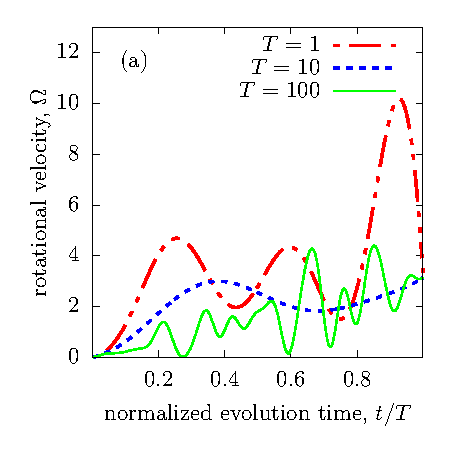
\includegraphics[width=0.45\textwidth]{data/1d/figR0.pdf}}
 \subfigure{
 \centering
 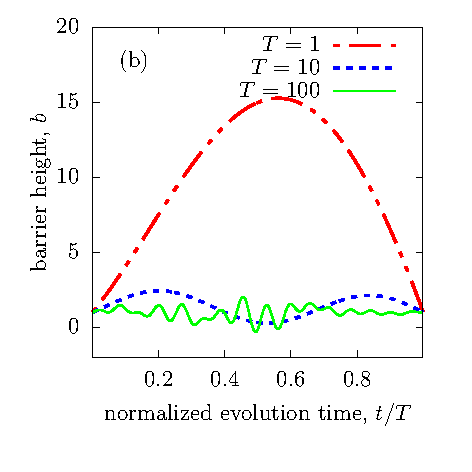
\includegraphics[width=0.45\textwidth]{data/1d/figB0.pdf}}
 \caption{Accelerating a single particle from the ground state with $J=15$.
 (a) Optimal rotational velocity pulses for $T = 1$, 10, and 100 for fixed barrier height $b=1$.
 (b) Optimal barrier height for a linearly increasing rotational velocity, $\Omega = \pi t/T$ for $T=1$, 10, and 100.}
 \label{fig:pulses}
\end{figure}

First, I will focus on the acceleration of a single particle, initially in the ground state of the system.
Figure~\ref{fig:pulses} (a) shows the results of this simulation if the barrier height is kept constant and one assumes an initial unmodified pulse that corresponds to a linear ramp from $\Omega = 0$ to $\pi$ for a preset total time, $T$.
For longer evolution times, there are many local maxima for the fidelity, and 
as such, longer evolution times effectively produce noisy signals and the Nelder--Mead method converges on one of many local minima.
For shorter evolution times, the pulse greatly affects the system and the shapes vary greatly from the initial linear ramp.
The infidelities for the linear guess pulse and its corresponding optimized pulse can be found in Figure~\ref{fig:lfid}, and one can see an improvement of several orders of magnitude.
Here, for longer evolution times, the initial linear pulse is a reasonable method to generate NOON states with an infidelity of $10^{-2}$ because it is already close to adiabatic; however, even in this case, the NOON state generation fidelity is better with optimization.
For all optimal control results in this chapter, the CRAB method was run 100 times and the data with the highest fidelity was kept.

For optimizations of the barrier strength, a simple linear ramp for $\Omega$ and an initial and final height for the barrier of $b = 1$ were chosen.
The optimal pulses for the barrier height for $T=1$, 10, and 100 are shown in Figure~\ref{fig:pulses}(b) and shorter evolution times similarly produce larger deviations from the initial pulse.
Again these pulses lead to significant improvements in the fidelity shown in Figure~\ref{fig:lfid}.

\begin{figure} 
\centering
 \subfigure{
 \centering
 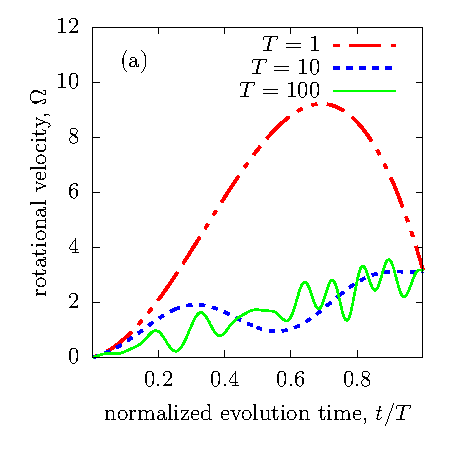
\includegraphics[width=0.45\textwidth]{data/1d/figR1.pdf}
 }
 \subfigure{
 \centering
 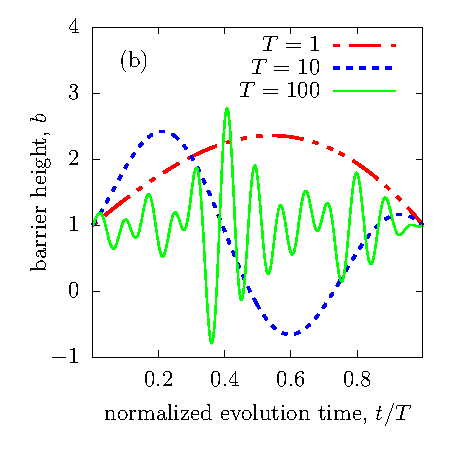
\includegraphics[width=0.45\textwidth]{data/1d/figB1.pdf}
 }
 \caption{
 Optimal pulses to accelerate a single particle initially in the ground state of the trap
 for $T = 1$, 10, and 100 for the (a) rotational velocity and (b) barrier height when optimizing over both simultaneously. }
 \label{fig:pulses_pair}
\end{figure}

With the CRAB method, it is possible to optimize over as many control parameters as one would like, and as such, it is possible to optimize over both the barrier strength and rotational frequency.
The results can be seen in Figure~\ref{fig:pulses_pair}, where (a) is the modified rotational frequency and (b) is the barrier height.
When comparing to the previous cases, similar trends emerge.
In particular, shorter evolution times result in less noisy optimizations when compared to longer evolution.
Even so, all sets of pulses are radically different when compared to optimizations over a single variable.
When comparing the fidelities in Figure~\ref{fig:lfid}, it is clear that optimizations over rotation alone provide the simplest method to optimize the fidelity.
It is likely that each run of the CRAB method is stuck in a local minimum in the fidelity landscape at some point and that optimization over both variables can provide the same optimization as rotating, alone.

\begin{figure}
 \centering 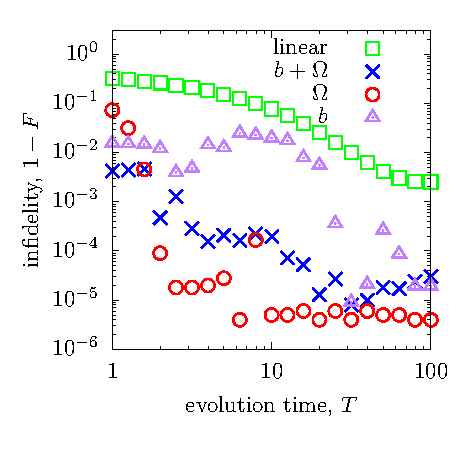
\includegraphics[width=0.5\textwidth]{data/1d/figlfid.pdf}
\caption{ Infidelities as a function of the overall process time for optimally controlled rotational acceleration, barrier height, or both.
Here, `linear' refers to an unoptimized linear acceleration from $\Omega = 0$ to $\pi$ while keeping the barrier height fixed at $b=1$.
}
\label{fig:lfid}
\end{figure}

\begin{figure}[t]
 \centering
 \subfigure{
 \centering
 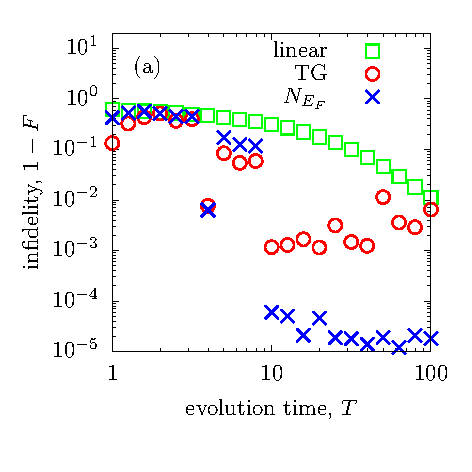
\includegraphics[width=0.45\textwidth]{data/1d/figTG3.pdf}
 }
 \subfigure{
 \centering
 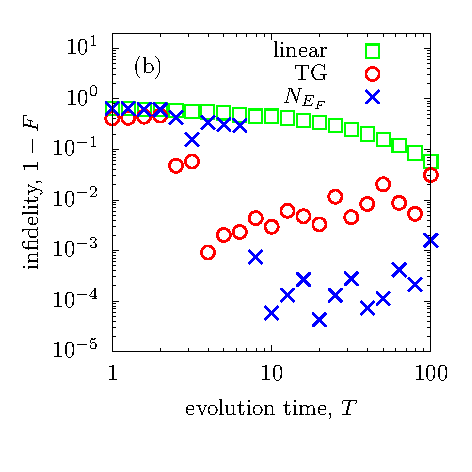
\includegraphics[width=0.45\textwidth]{data/1d/figTG5.pdf}
 }
 \caption{
Infidelities for the evolution of a TG gas with (a) $N=3$ and (b) $N=5$ particles using the CRAB optimal control technique.
The infidelities for optimized pulses with the particle at the Fermi edge is shown as blue crosses, and for the full TG gas as red circles.
Here, the green squares show the fidelity of a linear pulse for the atom closest to the Fermi edge.
A clear range where the CRAB algorithm is effective for generating NOON states with multiple particles can be clearly identified.}
 \label{fig:TGOC}
\end{figure} 


As such, when discussing the dynamics of a TG gas with 3 and 5 particles, I have only optimized over rotation.
Because of the Bose--Fermi mapping theorem, the evolution of an $N$-particle TG gas can be calculated by evolving a gas of $N$ spinless fermions.
In the zero-temperature limit, the fermions in the initial and target state create a Fermi sea by filling the lowest $N$ energy levels.
In this case, only atoms near the Fermi edge can transition into empty states and it is thus crucial to optimize the dynamics of the overall gas with respect to the particle with highest energy~\cite{garaot2015}.
In Figure~\ref{fig:TGOC}, I show the fidelity for the particle closest to the Fermi edge and the entire TG gas for $N=3$ and 5.
In this figure, one can see that by performing the optimization for the atoms near the Fermi edge, one can increase the fidelity of the entire gas for certain regimes; however, in contrast to Figure~\ref{fig:lfid}, there seems to be no fidelity increase from a linear pulse for short evolution times.
One can also observe what appears to be a crossover regime where optimizations of the particle at the Fermi edge seem to fail, but evolution of the entire gas is still slightly better than the linear pulse.
It is clear that the CRAB method creates highly effective pulses; however, for very short and long evolution times, the fidelity increase from a linear pulse is not as drastic.

\subsection{Results with STA protocols}

\begin{figure}
\centering
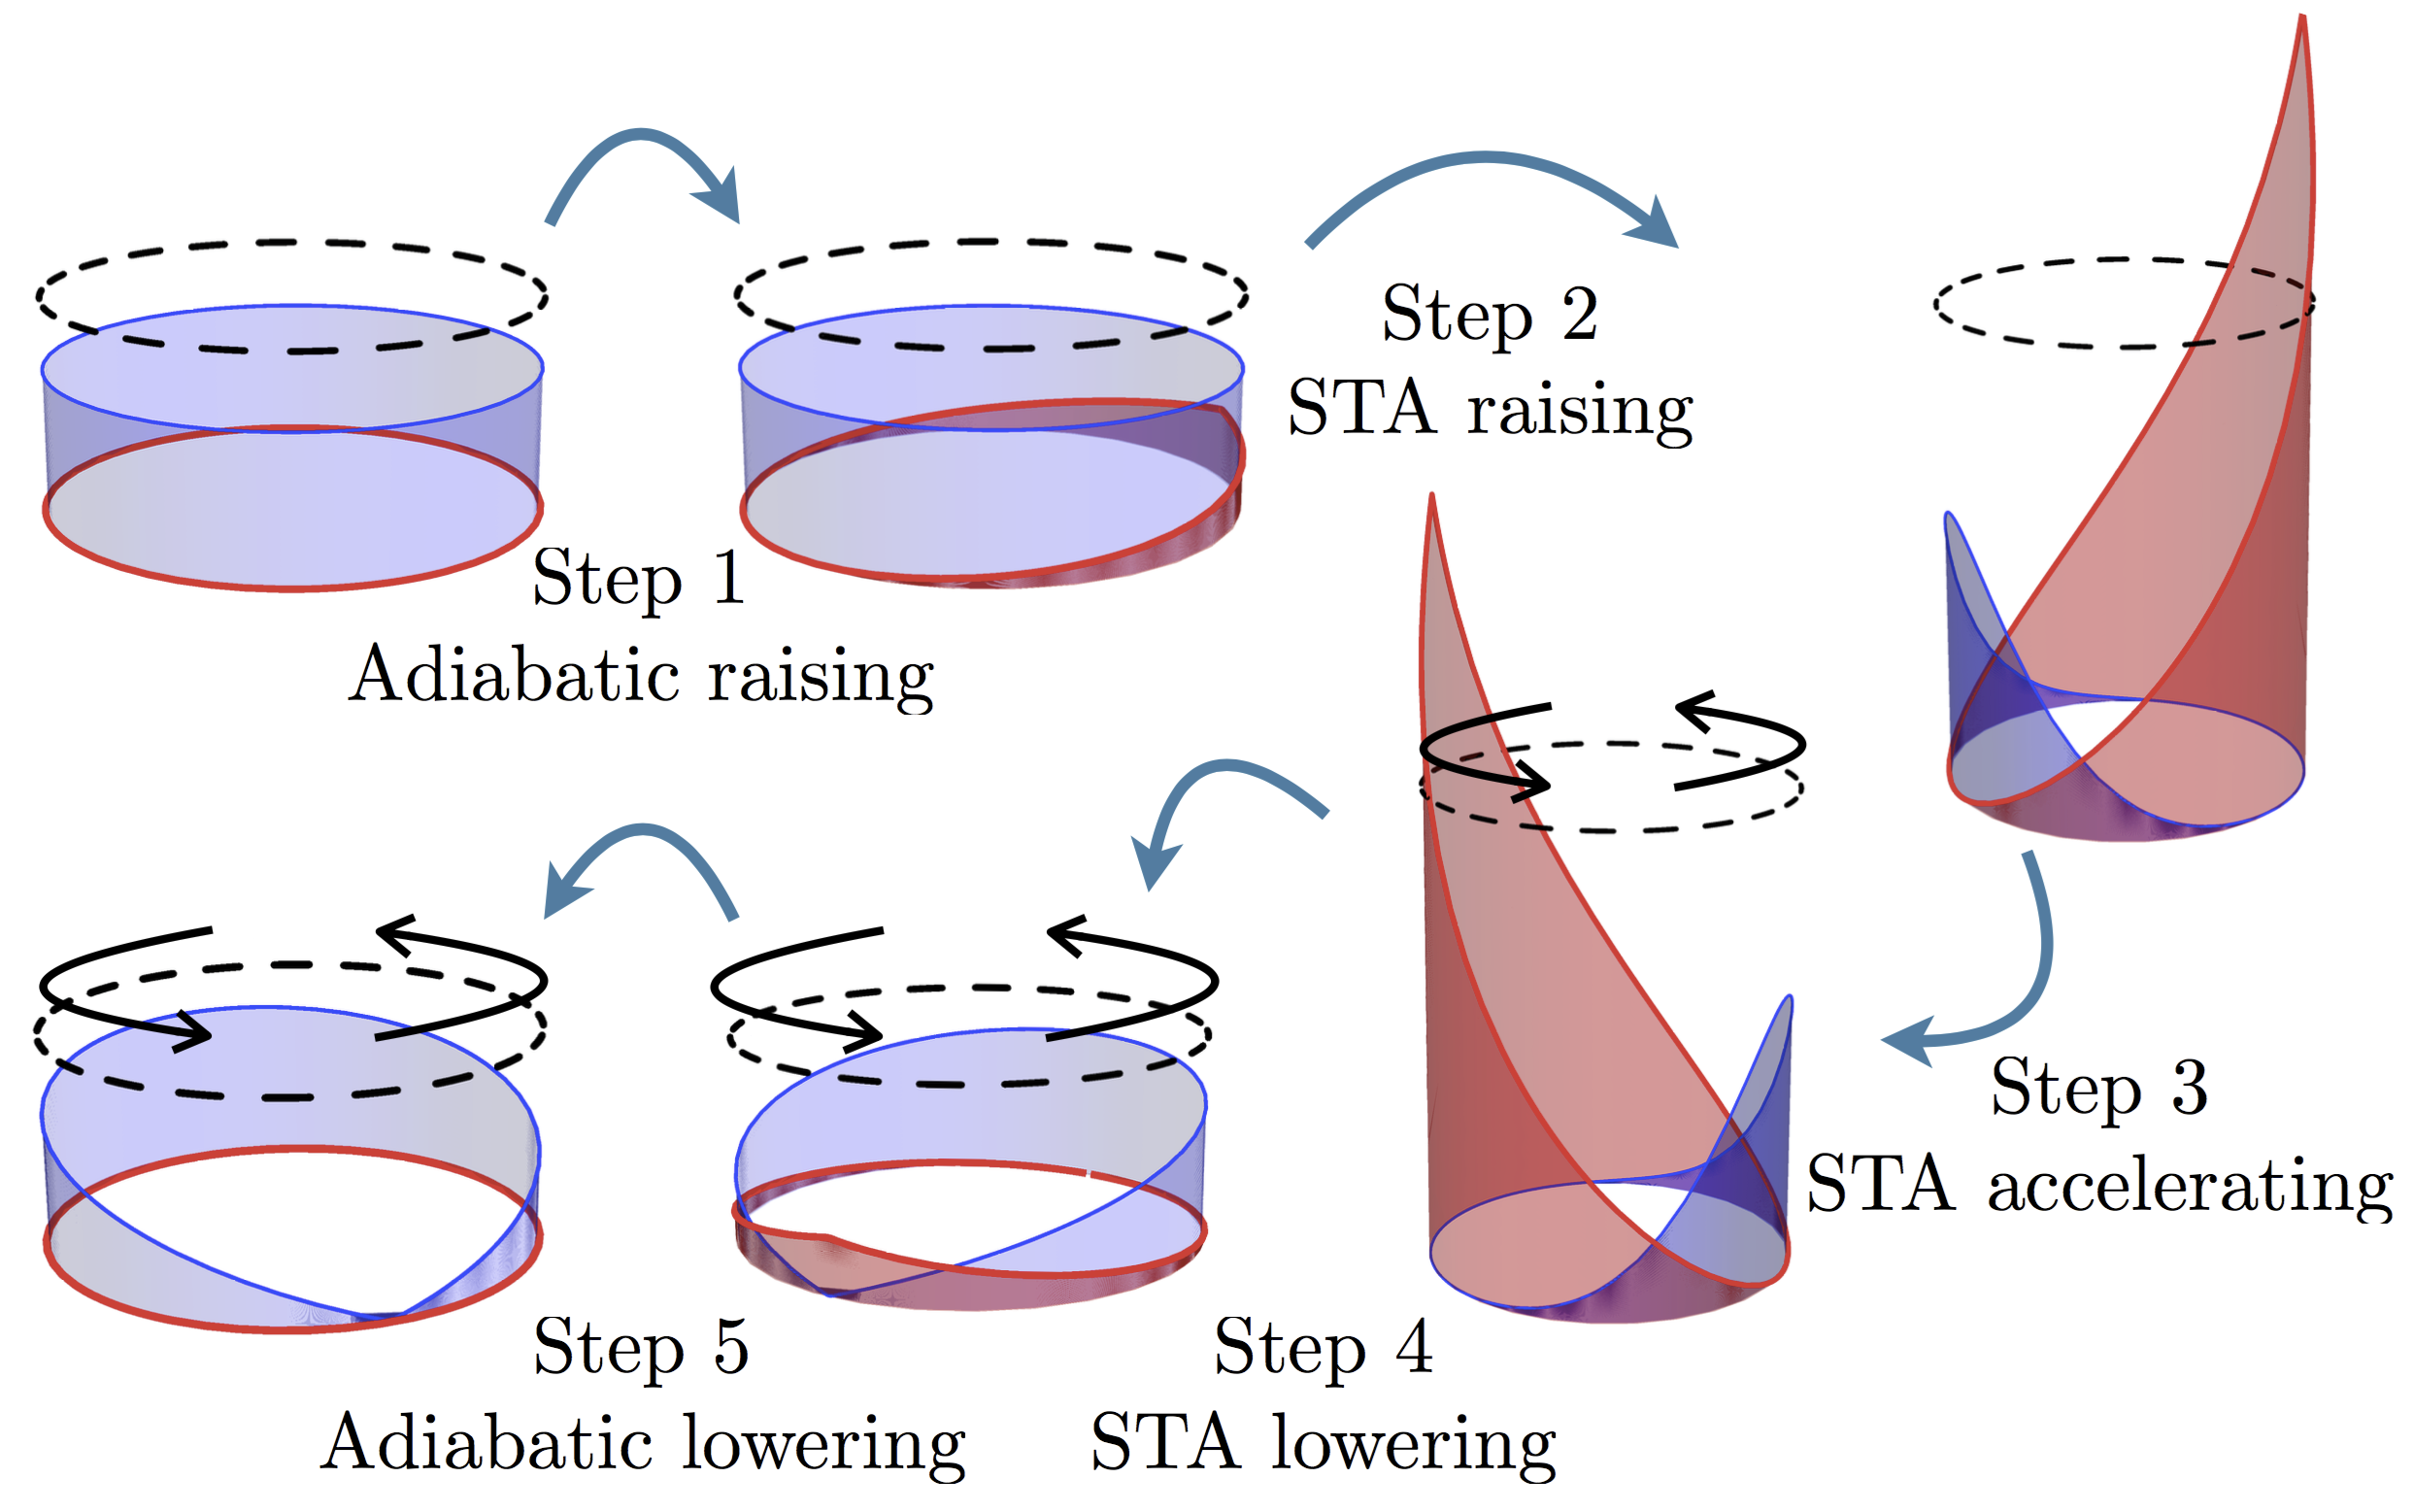
\includegraphics[width=0.8\textwidth]{data/1d/STAscheme.png} 
\caption{Scheme for the acceleration of a single atom using STA.
 In this example, the homogeneous ground state gets localized, accelerated and released at the angular velocity of $\Omega=\pi$ into the state
 $\left( \exp(i 2\pi x) +1 \right) /\sqrt 2$.
 The atomic density is indicated in blue and the potential is in red.}
\label{fig:STA-scheme}
\end{figure}


In this section, I will describe an STA protocol to generate NOON states in this system non-adiabatically, and though this was mentioned briefly in Section~\ref{sec:controltro}, it will be described more rigorously here.
In this case, I will start with rotational symmetry and break break this symmetry by introducing a time-dependent external potential at $t=0$ and removing it in the end.
For this, we do not choose a $\delta$ function, but instead a harmonic or sinusoidal potential along the ring.

The protocol consists of five steps:
\begin{enumerate}
\item Adiabatic raising of a weak harmonic or sinusoidal potential around the ring.
\item Fast tightening of this potential to localize the particles.
\item Accelerating the particles by moving the center of the potential.
\item Loosening the potential by reversing step 2.
\item Adiabatic lowering of the harmonic or sinusoidal potential.
\end{enumerate}
A schematic of this process is shown in Figure~\ref{fig:STA-scheme}.
For steps 2-4, pre-existing STA protocols can be used, and these will be discussed in this section.
The full protocol for the TG ring example will follow the STA methods outlined above with Lewis--Riesenfeld invariants and in this case, one needs to fulfill boundary conditions such that $\mathcal{\hat H}(t_0) = \mathcal{\hat H}(T)=p^2/2m$.
To be clear, the NOON states created with the STA protocol are slightly different those generated with quantum optimal control, as the STA variant does not rely on a $\delta$ barrier.

One of the two shortcuts explored for this system involves raising and lowering a harmonic potential~\cite{chen2010,chen20102}.
For this shortcut, a stationary harmonic potential is required and $F$, $x_c$, and $U$ from Equation~\eqref{eqn:HSTA} can all be set to zero, leading to
\begin{equation}
 \mathcal{\hat H}= -\frac{1}{2} \frac{\partial^2}{\partial x}+ \frac 1 2 \omega^2(t) x^2.
\end{equation}
\noindent To change the frequency while keeping the commutation relations and $\omega(t)$ continuous, one must impose the following conditions:
\begin{equation}
 \begin{array}{lcl}
\rho(t_0)=1, && \rho(t_f)=\gamma=\sqrt{\omega_0 / \omega_f},\\
\dot \rho(t_0)=0, && \dot \rho(t_f) =0, \\
\ddot \rho(t_0)=0, && \ddot \rho(t_f)=0.
\end{array} \label{eqn:squeeze}
\end{equation}

\noindent \noindent Which, together with Equations~\eqref{eqn:rho} and \eqref{eqn:squeeze} allow one to choose any form of $\rho$.
A good choice is the polynomial,
\begin{equation}
 \rho (s) = 6 \left(\gamma -1\right) s^5 -15 \left(\gamma-1\right) s^4 +10 \left(\gamma-1\right)s^3 + 1, \label{eq:rho_pol}
\end{equation}
\noindent where $s=(t-t_0)/(t_f-t_0)$ allows one to numerically find a solution for $\omega(t)$ that leads to the squeezing or expansion of the particle wavefunction with high fidelity in a short time.
As an important note, for small values of $\omega_0$, Equation~\eqref{eqn:rho} leads to purely imaginary values for $\omega(t)$, corresponding to repulsive potentials.
In order to avoid this and because the final states of this protocol require the external potential to be absent, the first and final steps in the protocol for this system involve adiabatically raising and lowering a potential to a suitable $\omega_0$ value. 

Once the potential has been raised, the particles are then accelerated to the chosen frequency, and a shortcut for this process with a harmonic trap exists~\cite{masuda2009,torrontegui2011,masuda2012}.
In the rotational shortcut, the trapping frequency is held constant and the position of the potential is modified.
This means that $U=0$, $F=\omega_0^2 x_0(t)$, and
\begin{equation}
 H= -\frac{1}{2} \frac{\partial^2}{\partial x}+ \frac 1 2 \omega^2_0 (x-x_0(t))^2.
\end{equation}
\noindent Here, Equation~\eqref{eqn:xc} becomes the only relevant auxiliary equation,
\begin{equation}
 \ddot{x}_c+\omega^2_0 (x_c-x_0)=0,
\end{equation}
and the conditions that must be imposed on $x_c$, are such that
\begin{equation}
 \begin{array}{lcl}
x_c(t_0)=x_0(t_0), && x_c(t_f)=d,\\
\dot x_c(t_0)=0, && \dot x_c(t_f) =\Omega_f, \\
\ddot x_c(t_0)=0, && \ddot x_c(t_f)=0,
\end{array}
\end{equation}
\noindent where $d$ is the final position of the potential minimum and $\Omega_f$ is its final velocity. 
For most applications of this shortcut, $d$ is important, and $\Omega_f$ is set to zero; however, this case is the opposite.

Like for the shortcut for raising the potential, the exact form of $x_c$ can be chosen somewhat arbitrarily, and a convenient choice is
\begin{equation}
 x_c(s)= (6 d -3 \Omega_f )s^5 - (15 d-7 \Omega_f )s^4+(10d-4 \Omega_f) s^3 + x_0(t_0),
\end{equation}
where, as above, $s$ is the normalized time.
The value of $\Omega_f$ can then be chosen to be odd multiples of $\pi$ to generate the desired NOON states based on the energy spectrum shown in Figure~\ref{fig:avoid}.

Unlike the shortcut to raise the potential, this shortcut is only approximate and works best when $\omega$ is large so that the particles are highly localized.
Both of these shortcuts rely on the presence of a harmonic potential of the form
\begin{equation}
 V_{H}(x,t)=\frac 1 2 \omega^2(t) \left( x-x_0(t)\right)^2, 
\end{equation}
where  $\omega$ is the frequency of the trap (in units of $\hbar/mL^2$) and $x_0$ the position of its minimum.
In the case of the TG ring, the potential must be symmetric around $x_0$, such that it is continuous at $x=\pm 1/2$; therefore, the real form of $(x-x_0)$ must be $(x-x_0+1/2)(\mathrm{mod~} 1)-1/2$.
The potential $V_H$ is then continuous everywhere on the ring, but its derivative is discontinuous at $x=x_0+1/2$ because this position is diametrically opposite to $x_0$.
Though $V_H$ is easy to work with theoretically, it is not necessarily experimentally realistic, and for this reason, we also consider a sinusoidal potential of the form~\cite{phelan2013,masuda2014},
\begin{equation}
 V_{S}(x,t)= \frac{\omega^2(t)}{2 \pi^2} \sin^2 \left(\pi \left( x-x_0(t)\right) \right) ,
\end{equation}
where the notation is the same as before. 
Here, prefactors are chosen such that $V_{H}$ is an approximation of $V_S$ around $x_0$.

\begin{figure}
\centering
\subfigure{
\centering
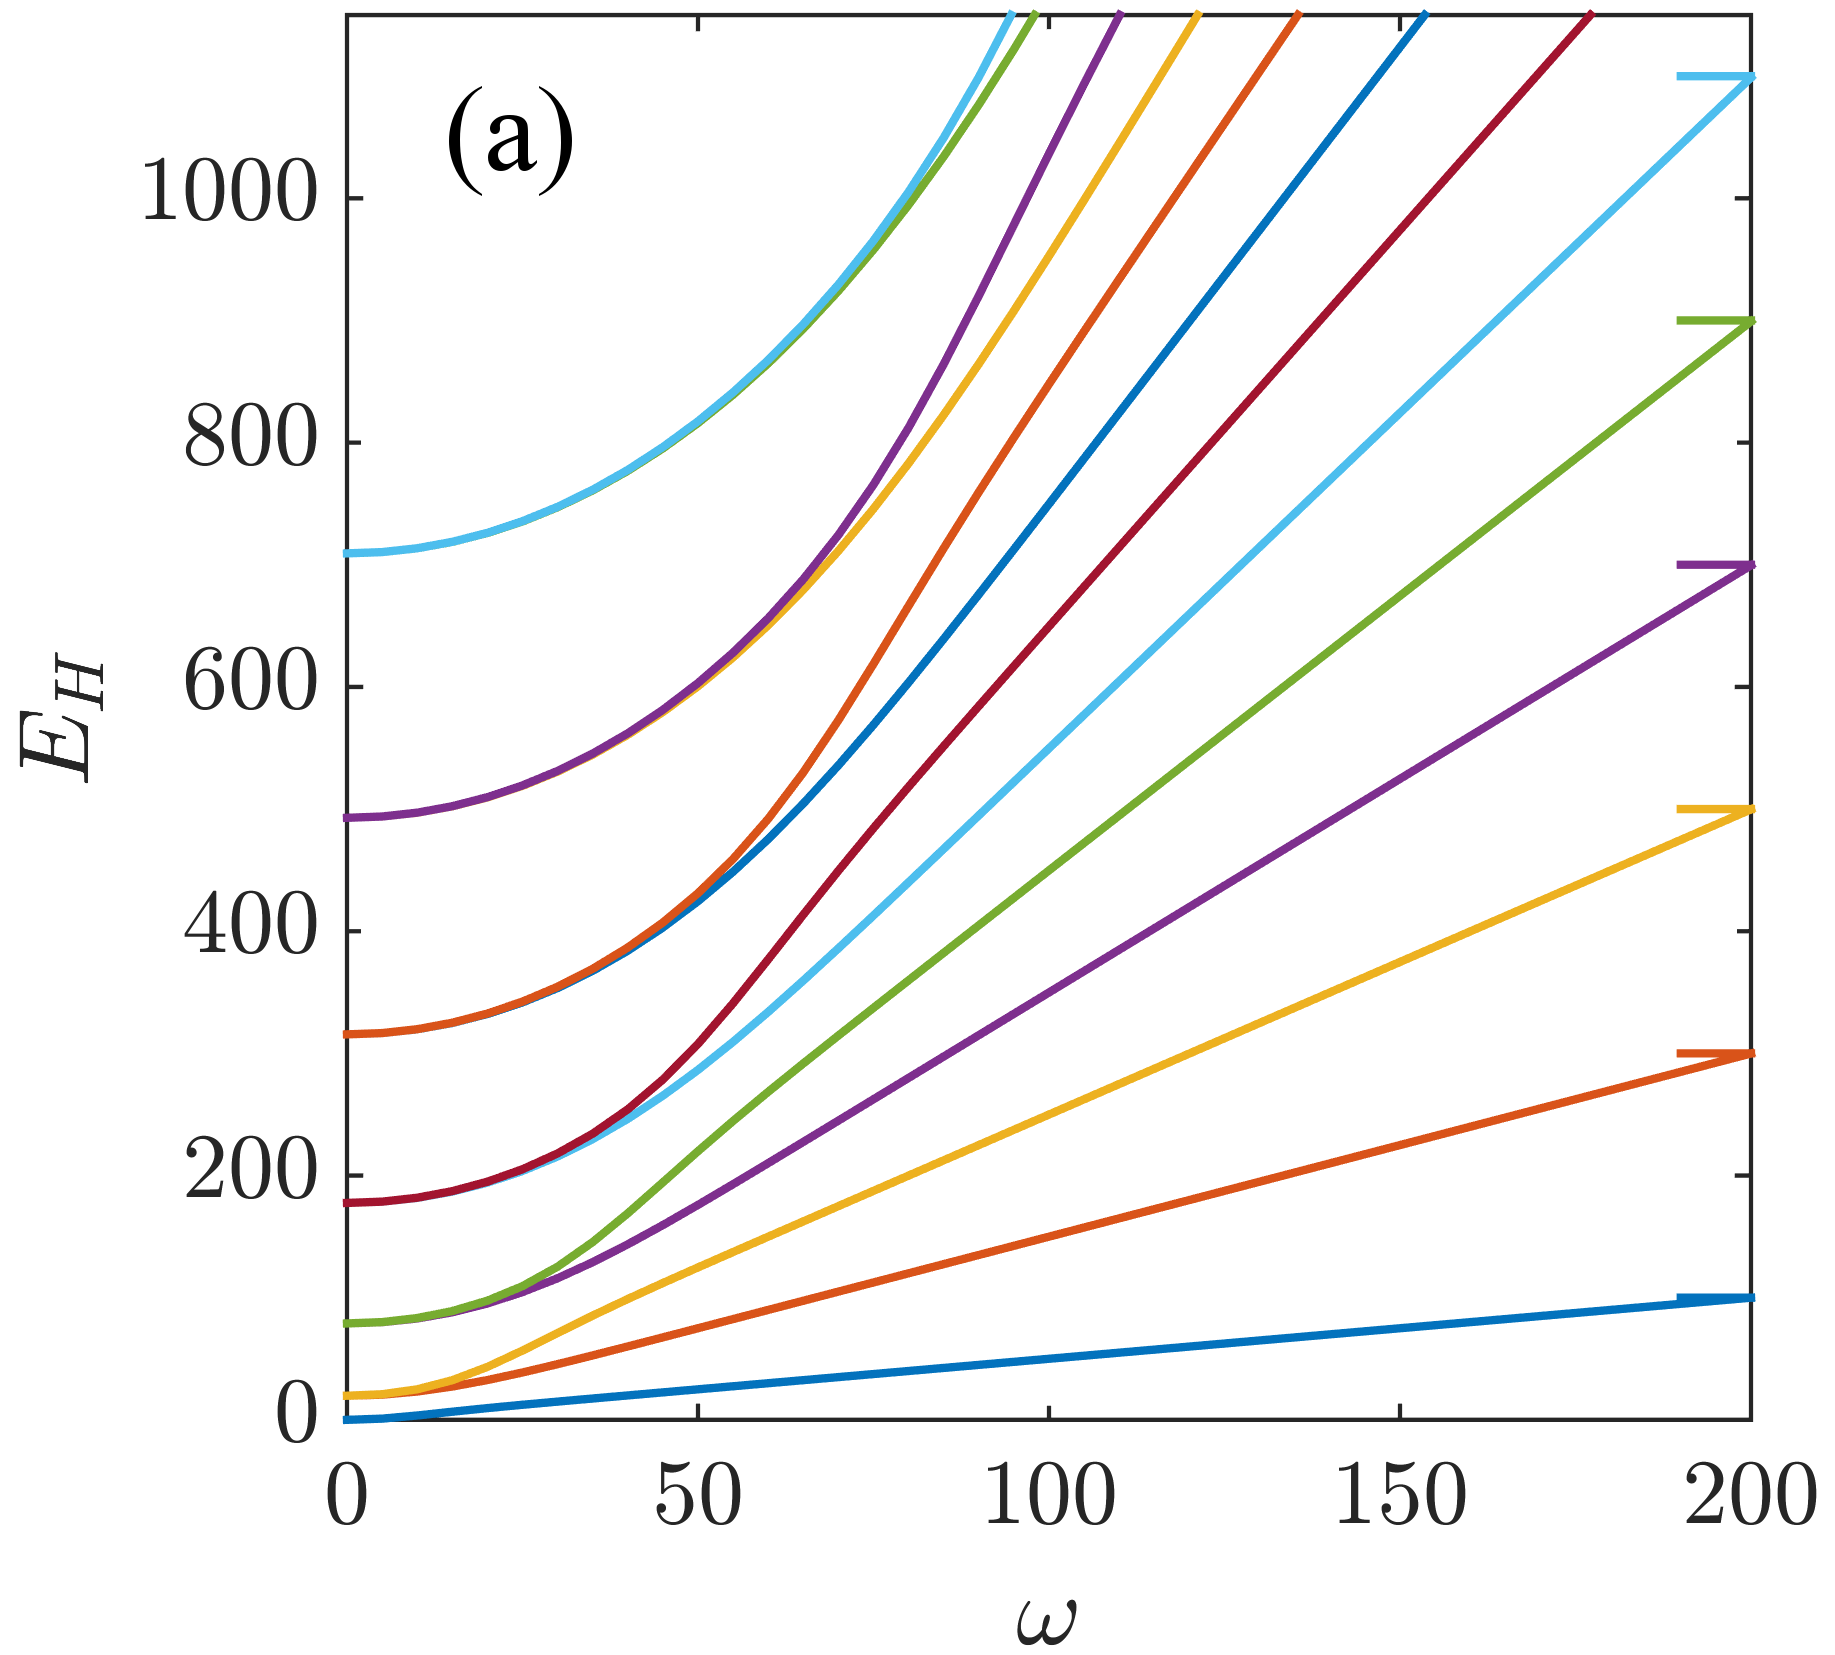
\includegraphics[width=0.48\linewidth]{data/1d/fig1.png}}
\subfigure{
\centering
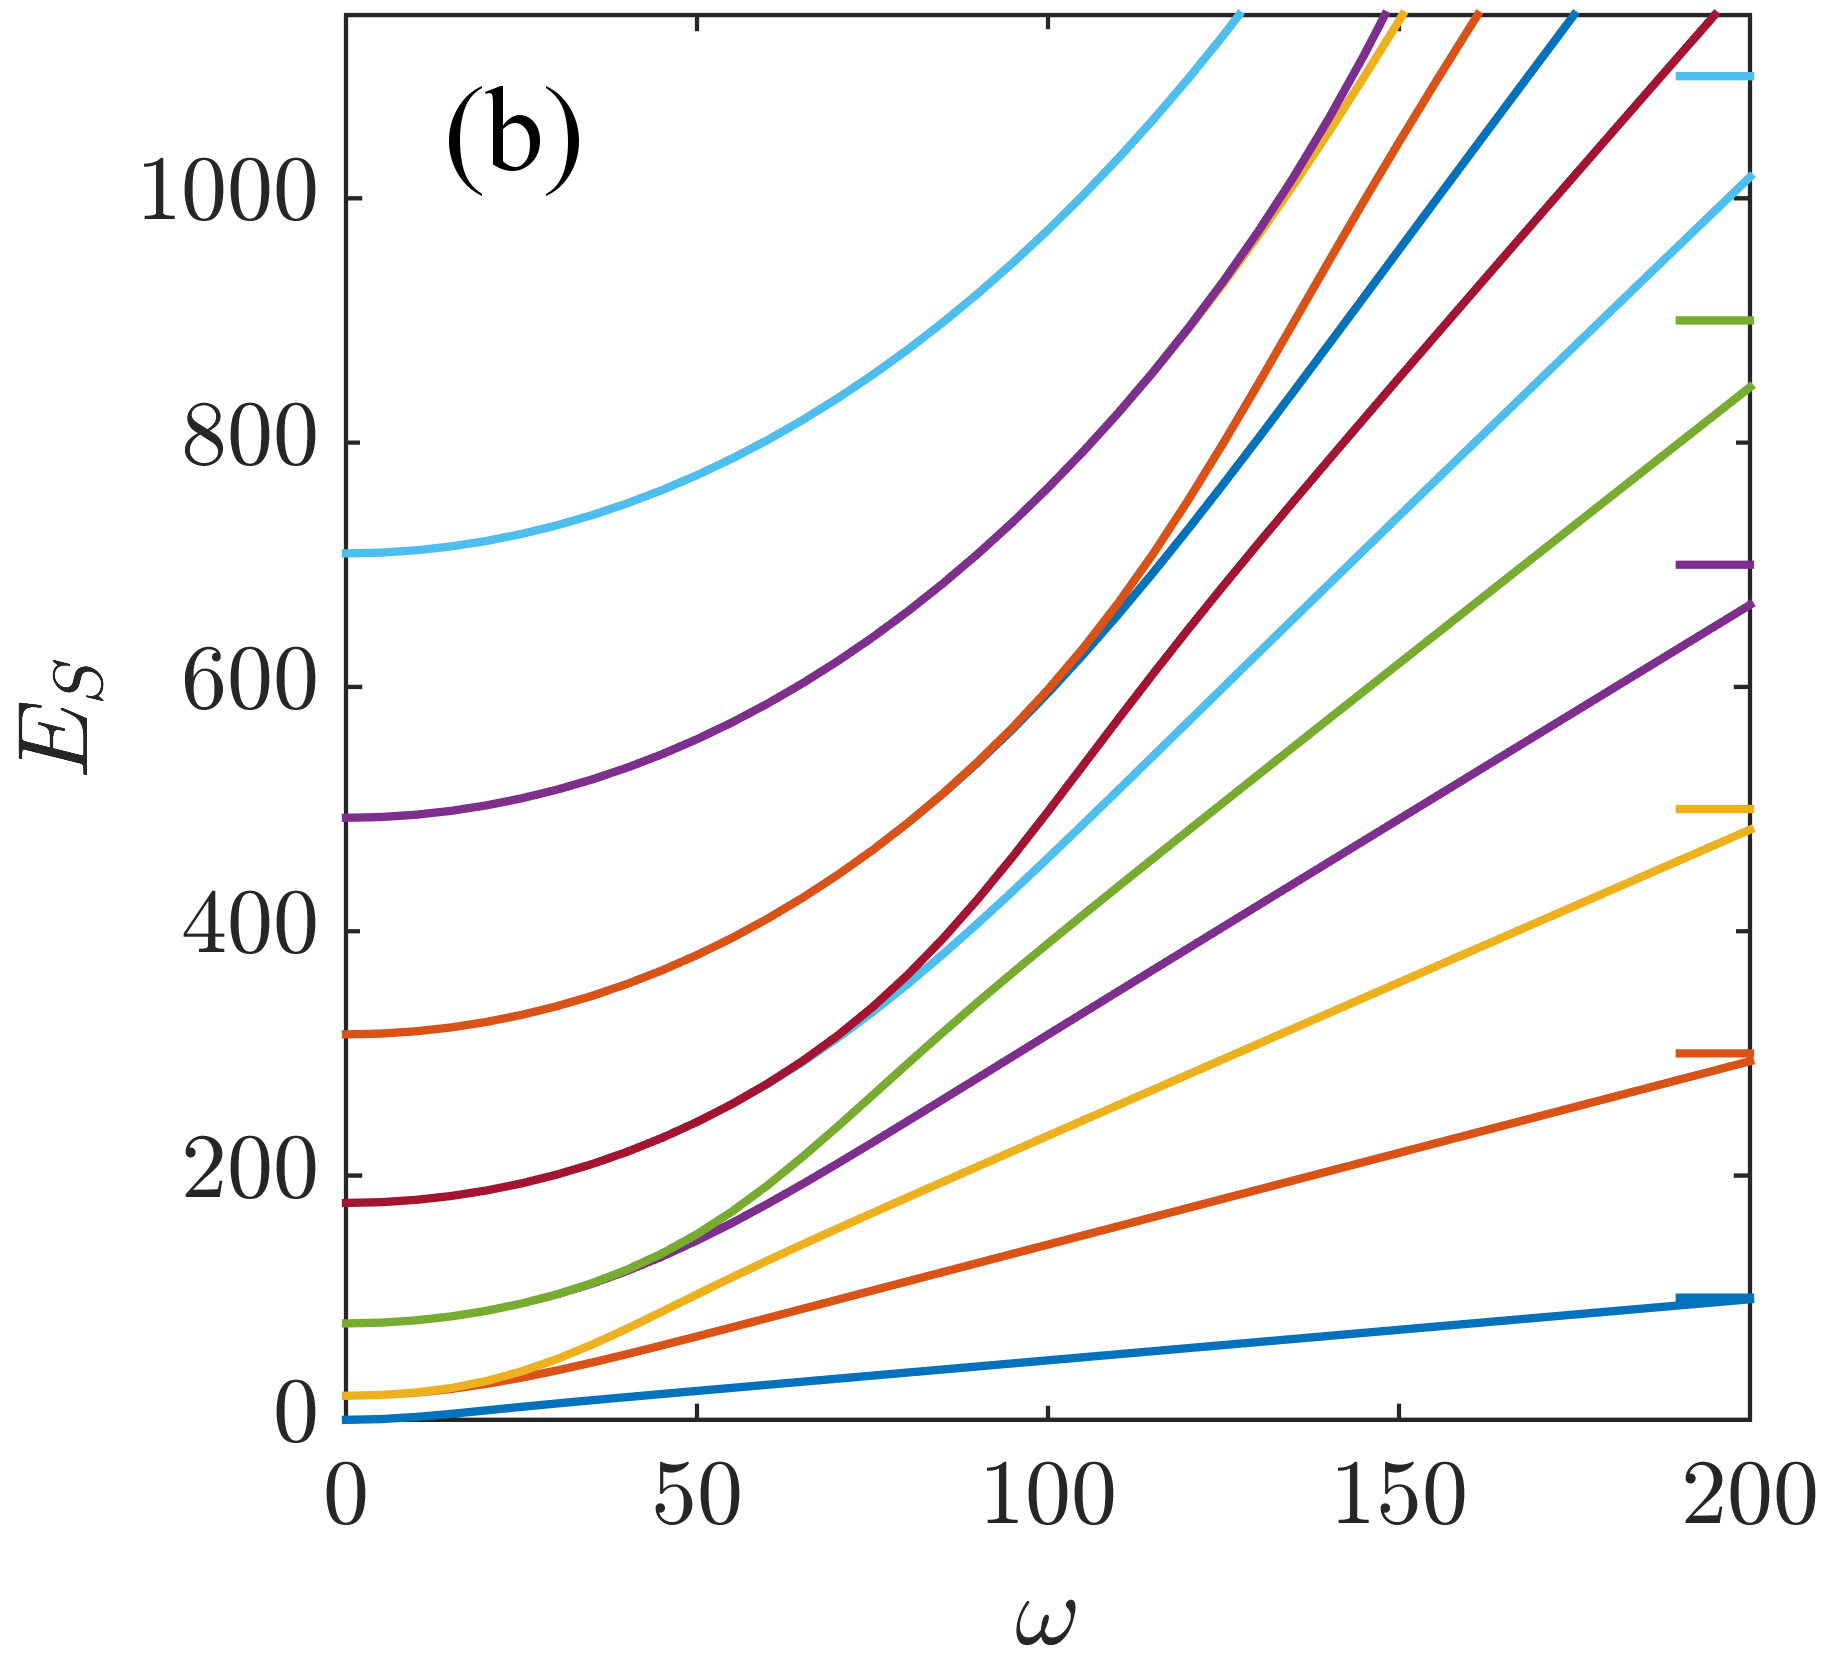
\includegraphics[width=0.48\linewidth]{data/1d/fig2.png}}

\caption{ Energy eigenspectrum of the system with (a) a harmonic or (b) a sinusoidal potential as a function of $\omega$. 
The eigenstates continuously change from angular momentum states of energy $E_k=2\pi^2 k^2$ (with $k=0,\pm1,\ldots$) at $\omega=0$, towards harmonic-oscillator states of energy $E_n=\omega(n+1/2)$ (with $n=0,1,\ldots$) for large $\omega$.
For comparison, the horizontal lines on the right vertical axis give the energy levels in a harmonic potential with $\omega=200$.}
\label{fig:spectrum}
\end{figure}

In Figure~\ref{fig:spectrum}, I show the difference between the two potentials by computing the energy spectra of both Hamiltonians.
Here, the eigenstates at $\omega=0$ are the angular momentum states $e^{i 2 \pi k x}$, with degenerate clockwise and counterclockwise momentum states of opposite quantum number $k$.
As $\omega$ is increased, the degeneracy ceases and the spectrum asymptotically approaches that of a harmonic oscillator.
For the sinusoidal case, the difference with the harmonic spectrum increases with the quantum number $n$.

\begin{figure}
\centering
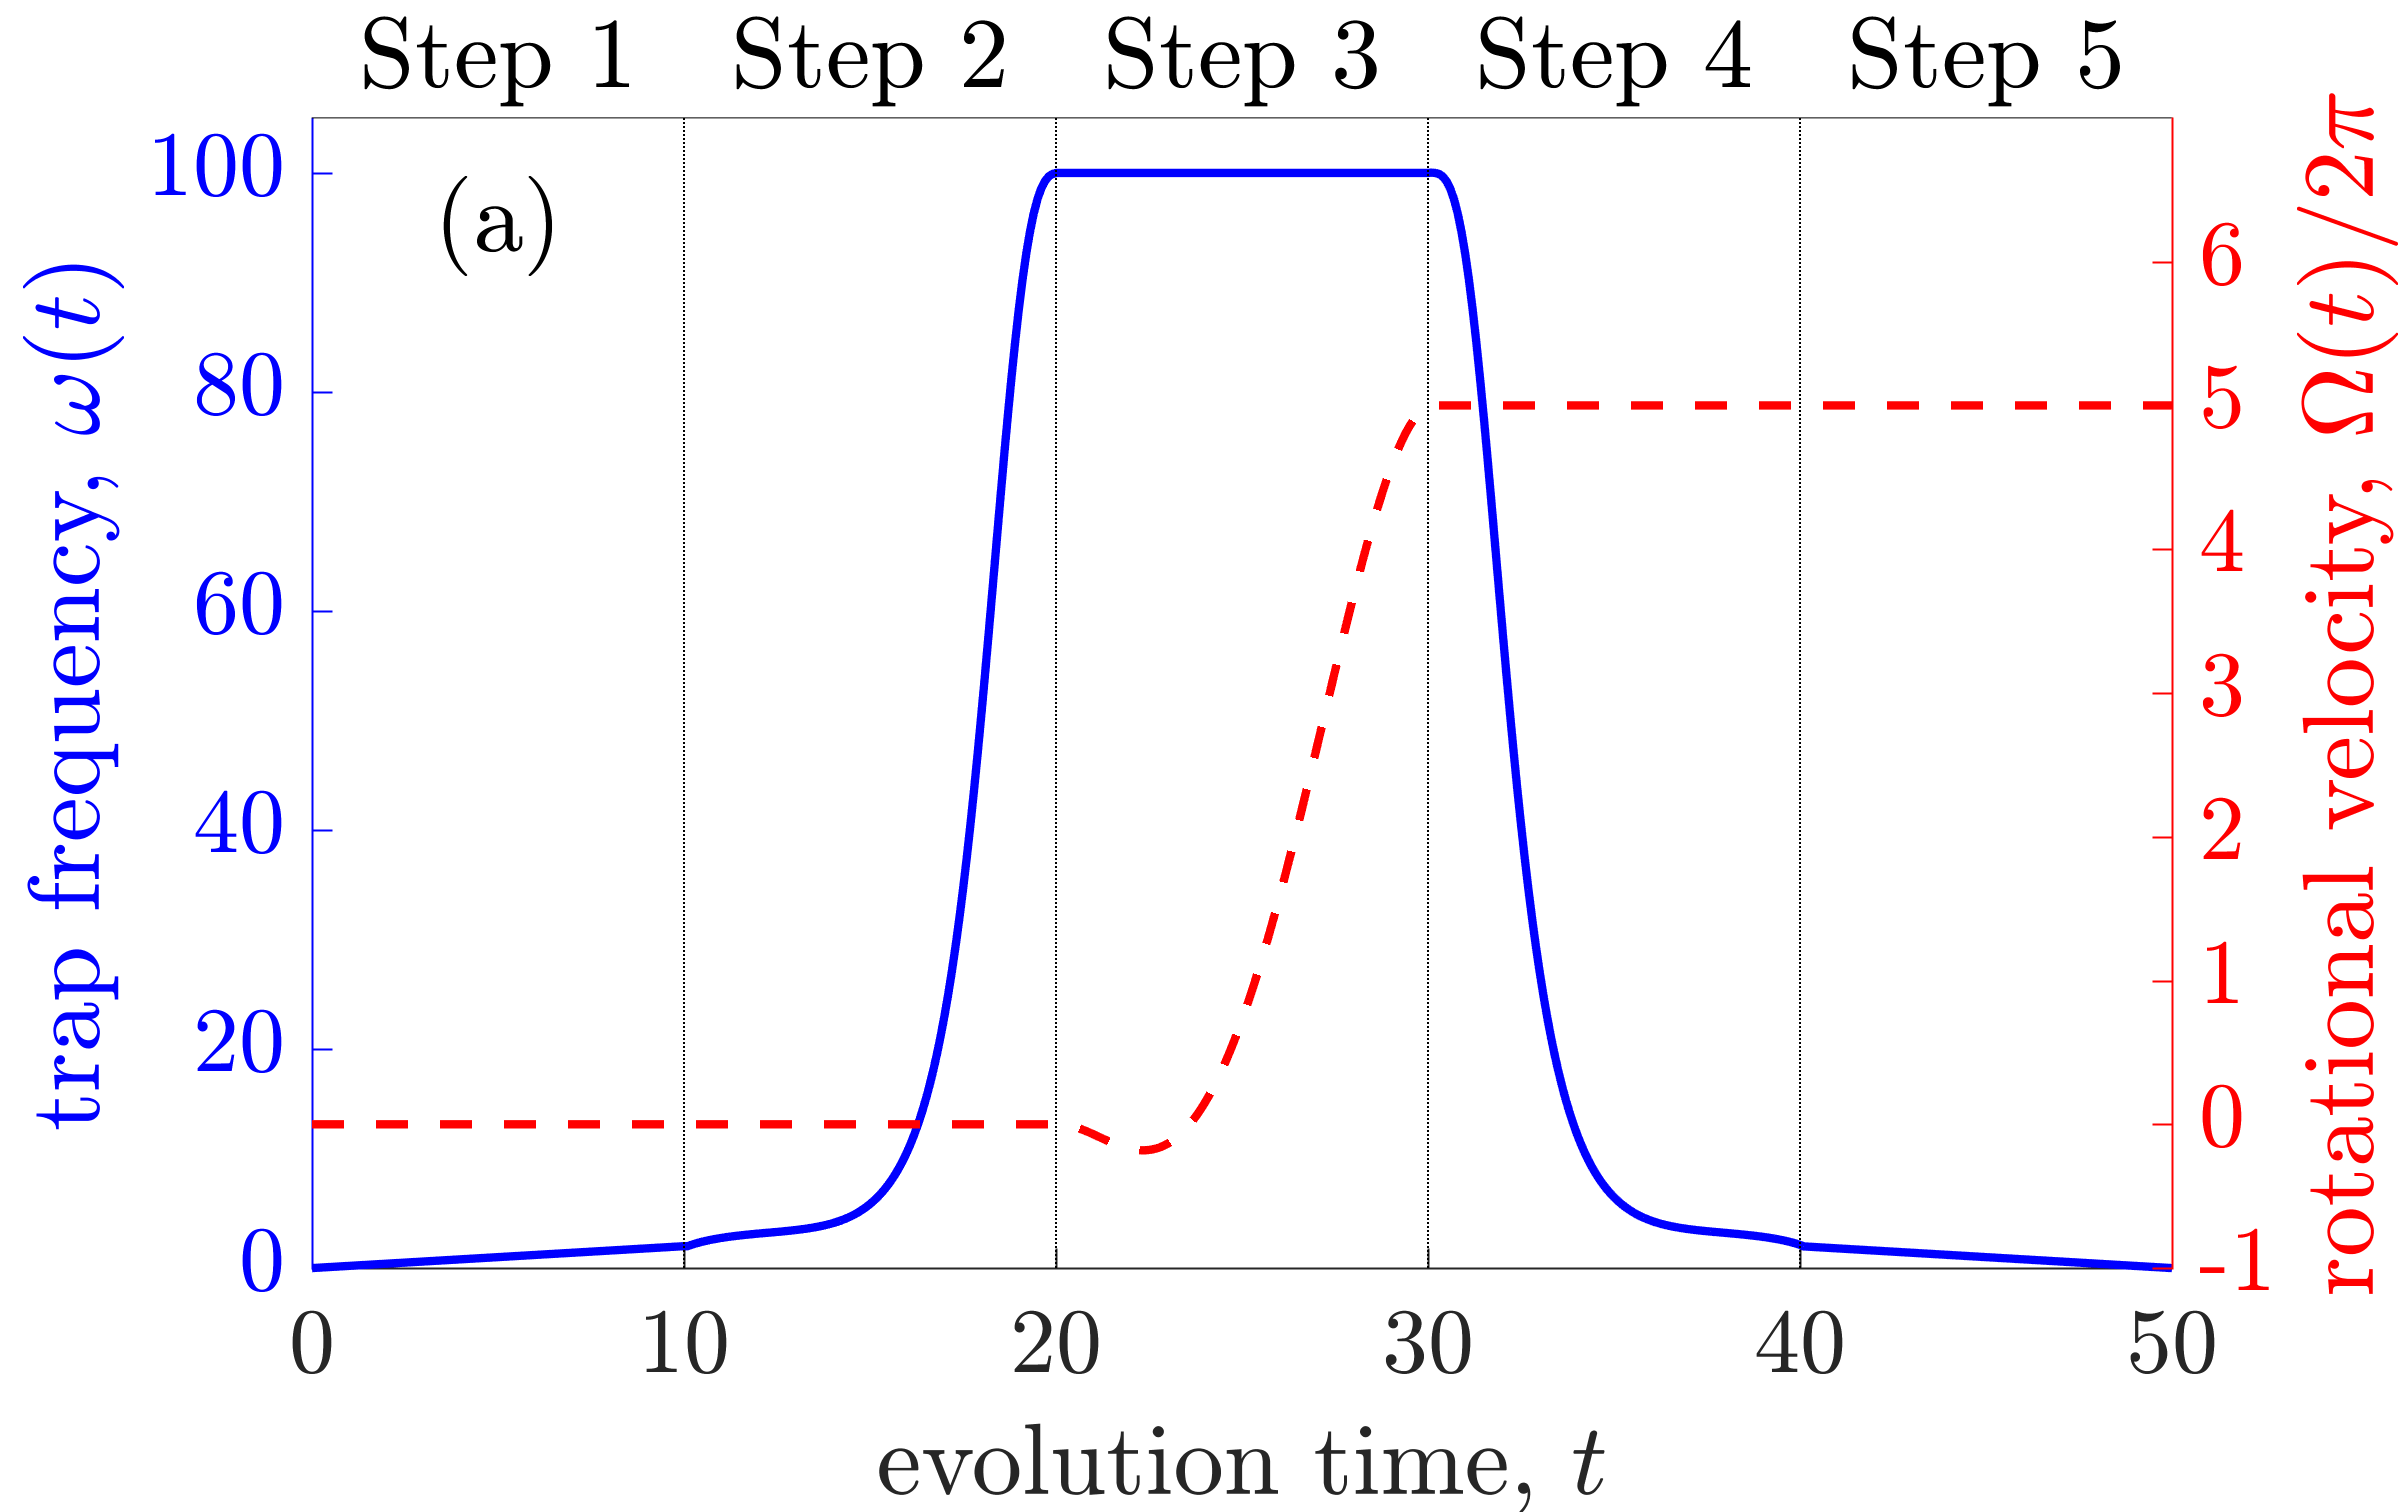
\includegraphics[width=0.45\linewidth]{data/1d/fig5.png}
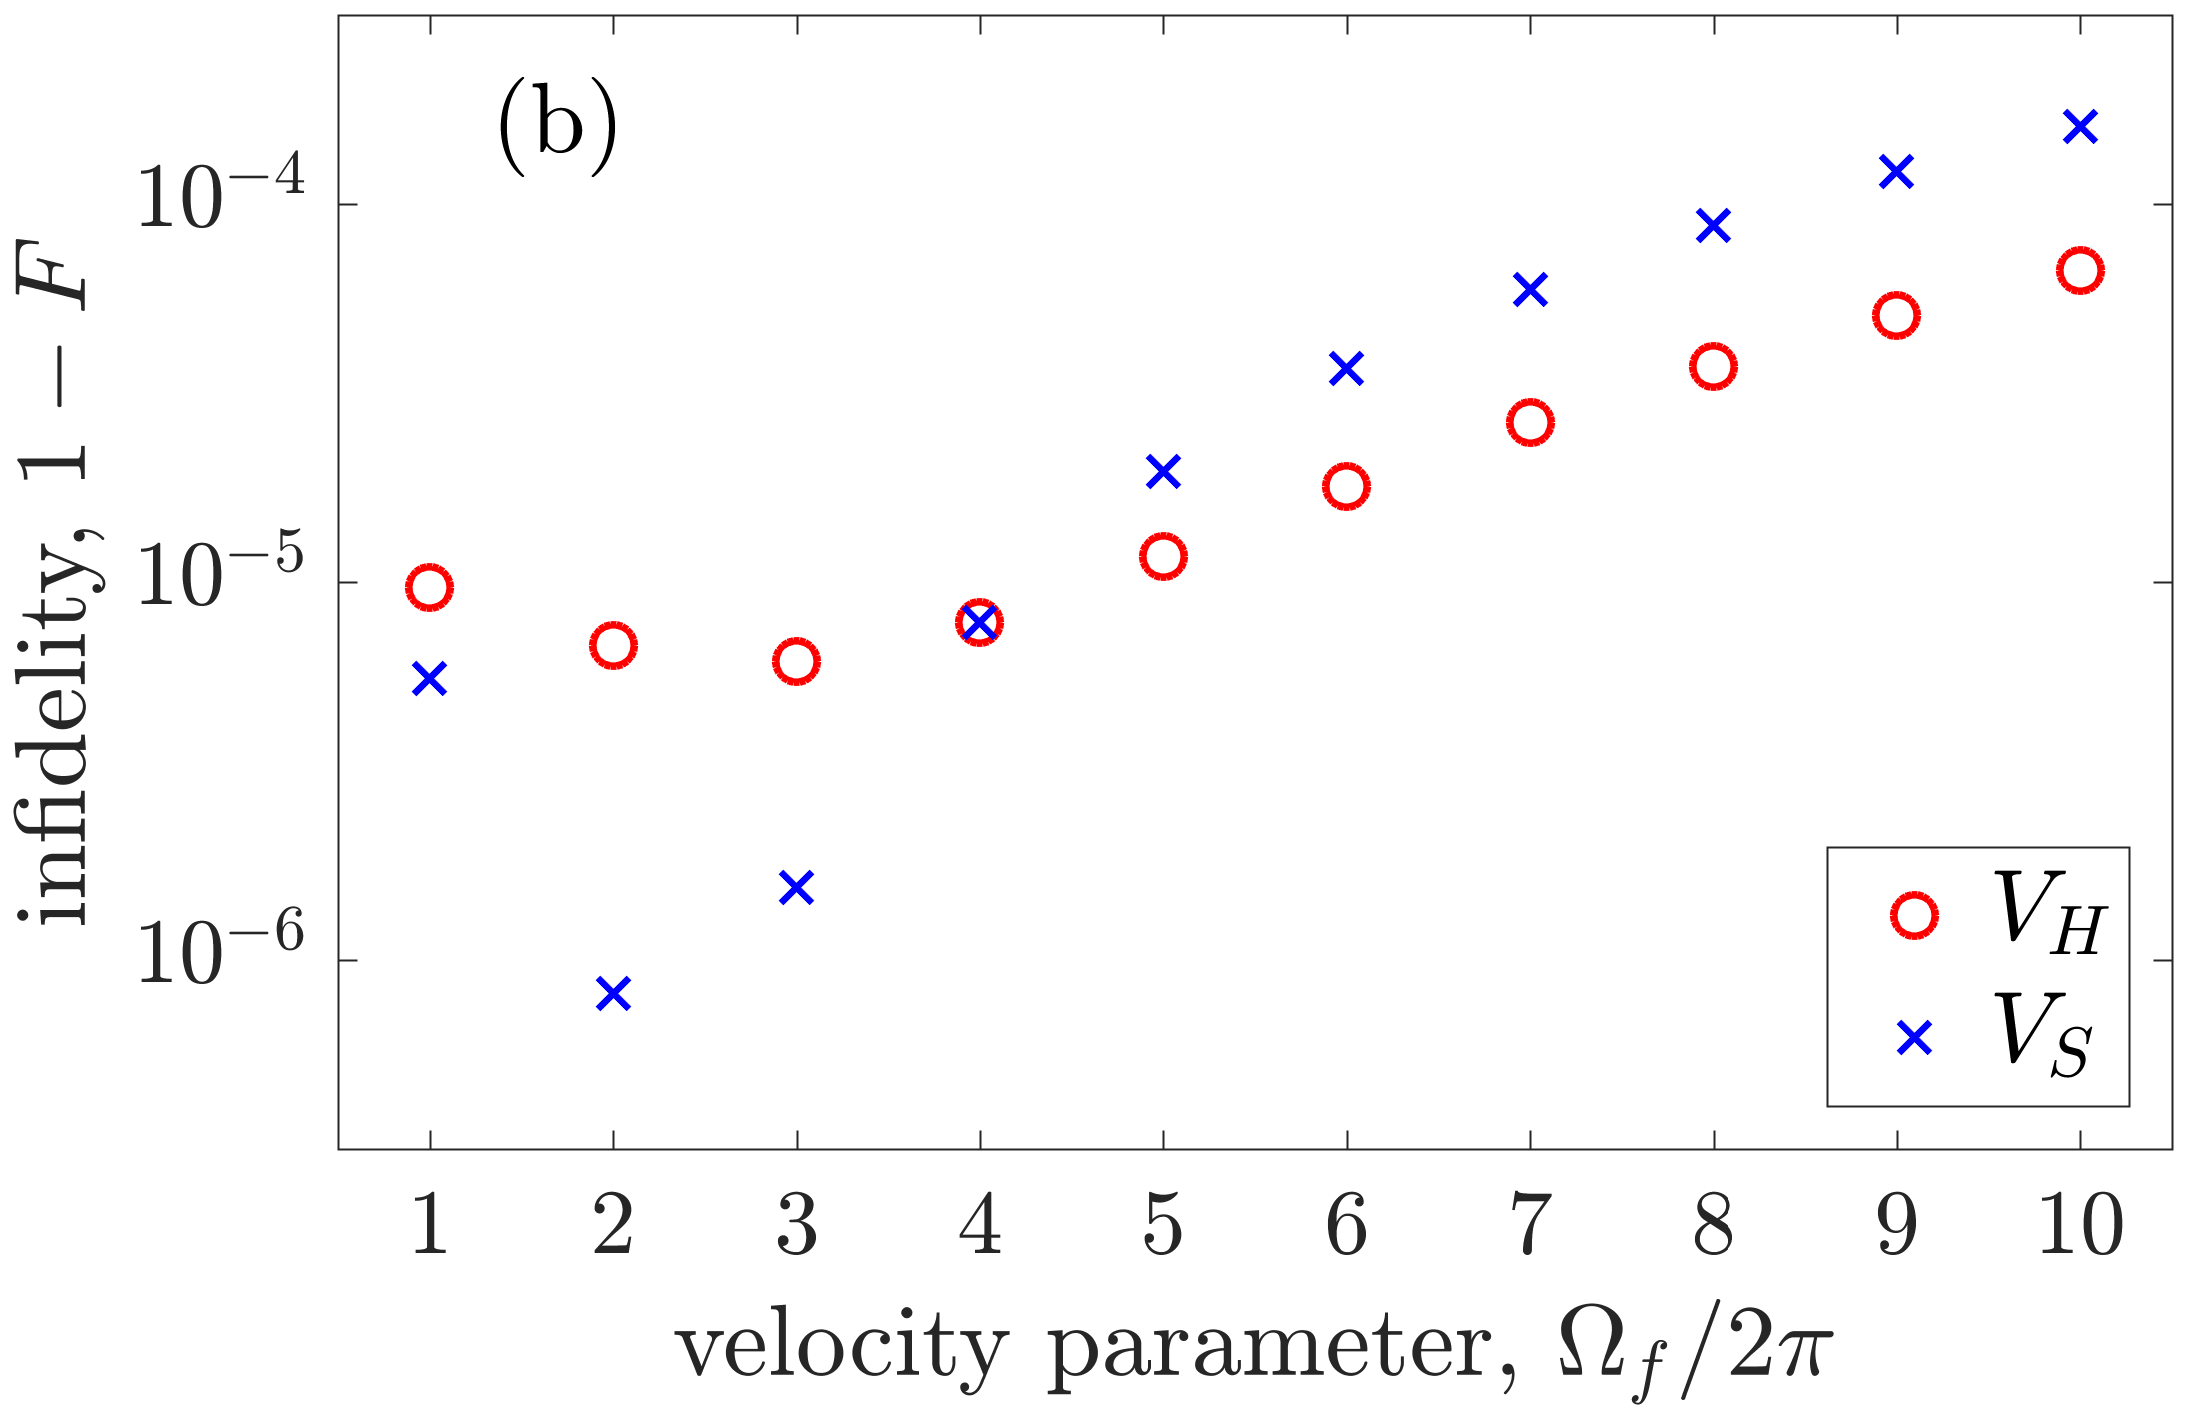
\includegraphics[width= 0.45\linewidth]{data/1d/fig6.png}
\caption{
(a) Plot of the parameters $\omega(t)$ and the angular velocity $\Omega(t)$ for the entire protocol.
The parameters are $\omega_0=2$, $\omega_f=100$, $d=100$, each step is executed in $t_f-t_0=10$, and $\Omega_f$ is picked depending on the desired output state (here, $\Omega_f=5 \times 2\pi$).
(b) Final infidelities for $\Omega_f=1,2,\ldots,10 \times 2\pi$ for $V_H$ (dotted blue line) and $V_S$ (solid red line).
The rest of parameters are as shown in (a).
}
\label{fig:final+param}
\end{figure}

Like the case of quantum optimal control, I will first show the single-particle results.
In Figure~\ref{fig:final+param}(a), the values for $\omega(t)$ and $\Omega(t)$ are shown, and
in Figure~\ref{fig:final+param}(b), the infidelities for the state preparation of plane waves $e^{i \Omega_f x}$ with $\Omega_f=1\ldots10 \times 2 \pi$ are shown.
Here, it is clear that even for a large amount of angular momentum, the fidelities remain high for both the harmonic and sinusoidal potentials.

For a multi-particle case in the TG regime, the initial states for the particles will be eigenstates of free space, which are simply plane waves $e^{i 2 \pi k x}$ with integer $k$.
Because the states with $\pm k$ are degenerate, it is equally valid to consider the initial eigenstates
\begin{align}
\phi^i_0(x)&=1,\\
\phi^i_{2l-1}(x)&=\frac{1}{\sqrt 2} \left( e^{i 2 \pi l x}-e^{-i 2 \pi l x} \right)= i \sqrt{2} \sin(2 l \pi x), \\
\phi^i_{2l}(x)&= \frac{1}{\sqrt 2}\left( e^{i 2 \pi l x}+e^{-i 2 \pi l x} \right) = \sqrt{2} \cos(2 l \pi x),
\end{align}
for $l=\{1,2,\ldots\}$.
These states have a total angular momentum of zero and are well-suited for the provided STA protocol because when an odd number of particles occupies the lower eigenstates, the sine and cosine pairs are guaranteed to be populated.

For $\Omega_f=\pi$, the plane wave of quantum numbers $k+1$ and $-k$ are degenerate and one can construct the target states
\begin{align}
\phi^t_{2l}(x)&=\frac{1}{\sqrt 2} \left( e^{i 2 \pi (l+1) x} + e^{-i 2 \pi l x} \right) = \sqrt{2} \cos[(2l+1) \pi x] e^{i \pi x} , \\
\phi^t_{2l+1}(x)&=\frac{1}{\sqrt 2} \left( e^{i 2 \pi (l+1) x}-e^{-i 2 \pi l x} \right) = i \sqrt{2} \sin[(2l+1) \pi x]e^{i \pi x} ,
\end{align}
for $l=\{0,1,2,\ldots\}$.
The states with total angular momentum $\pi$ are similar to NOON states.

\begin{figure}
\centering
\subfigure{
\centering
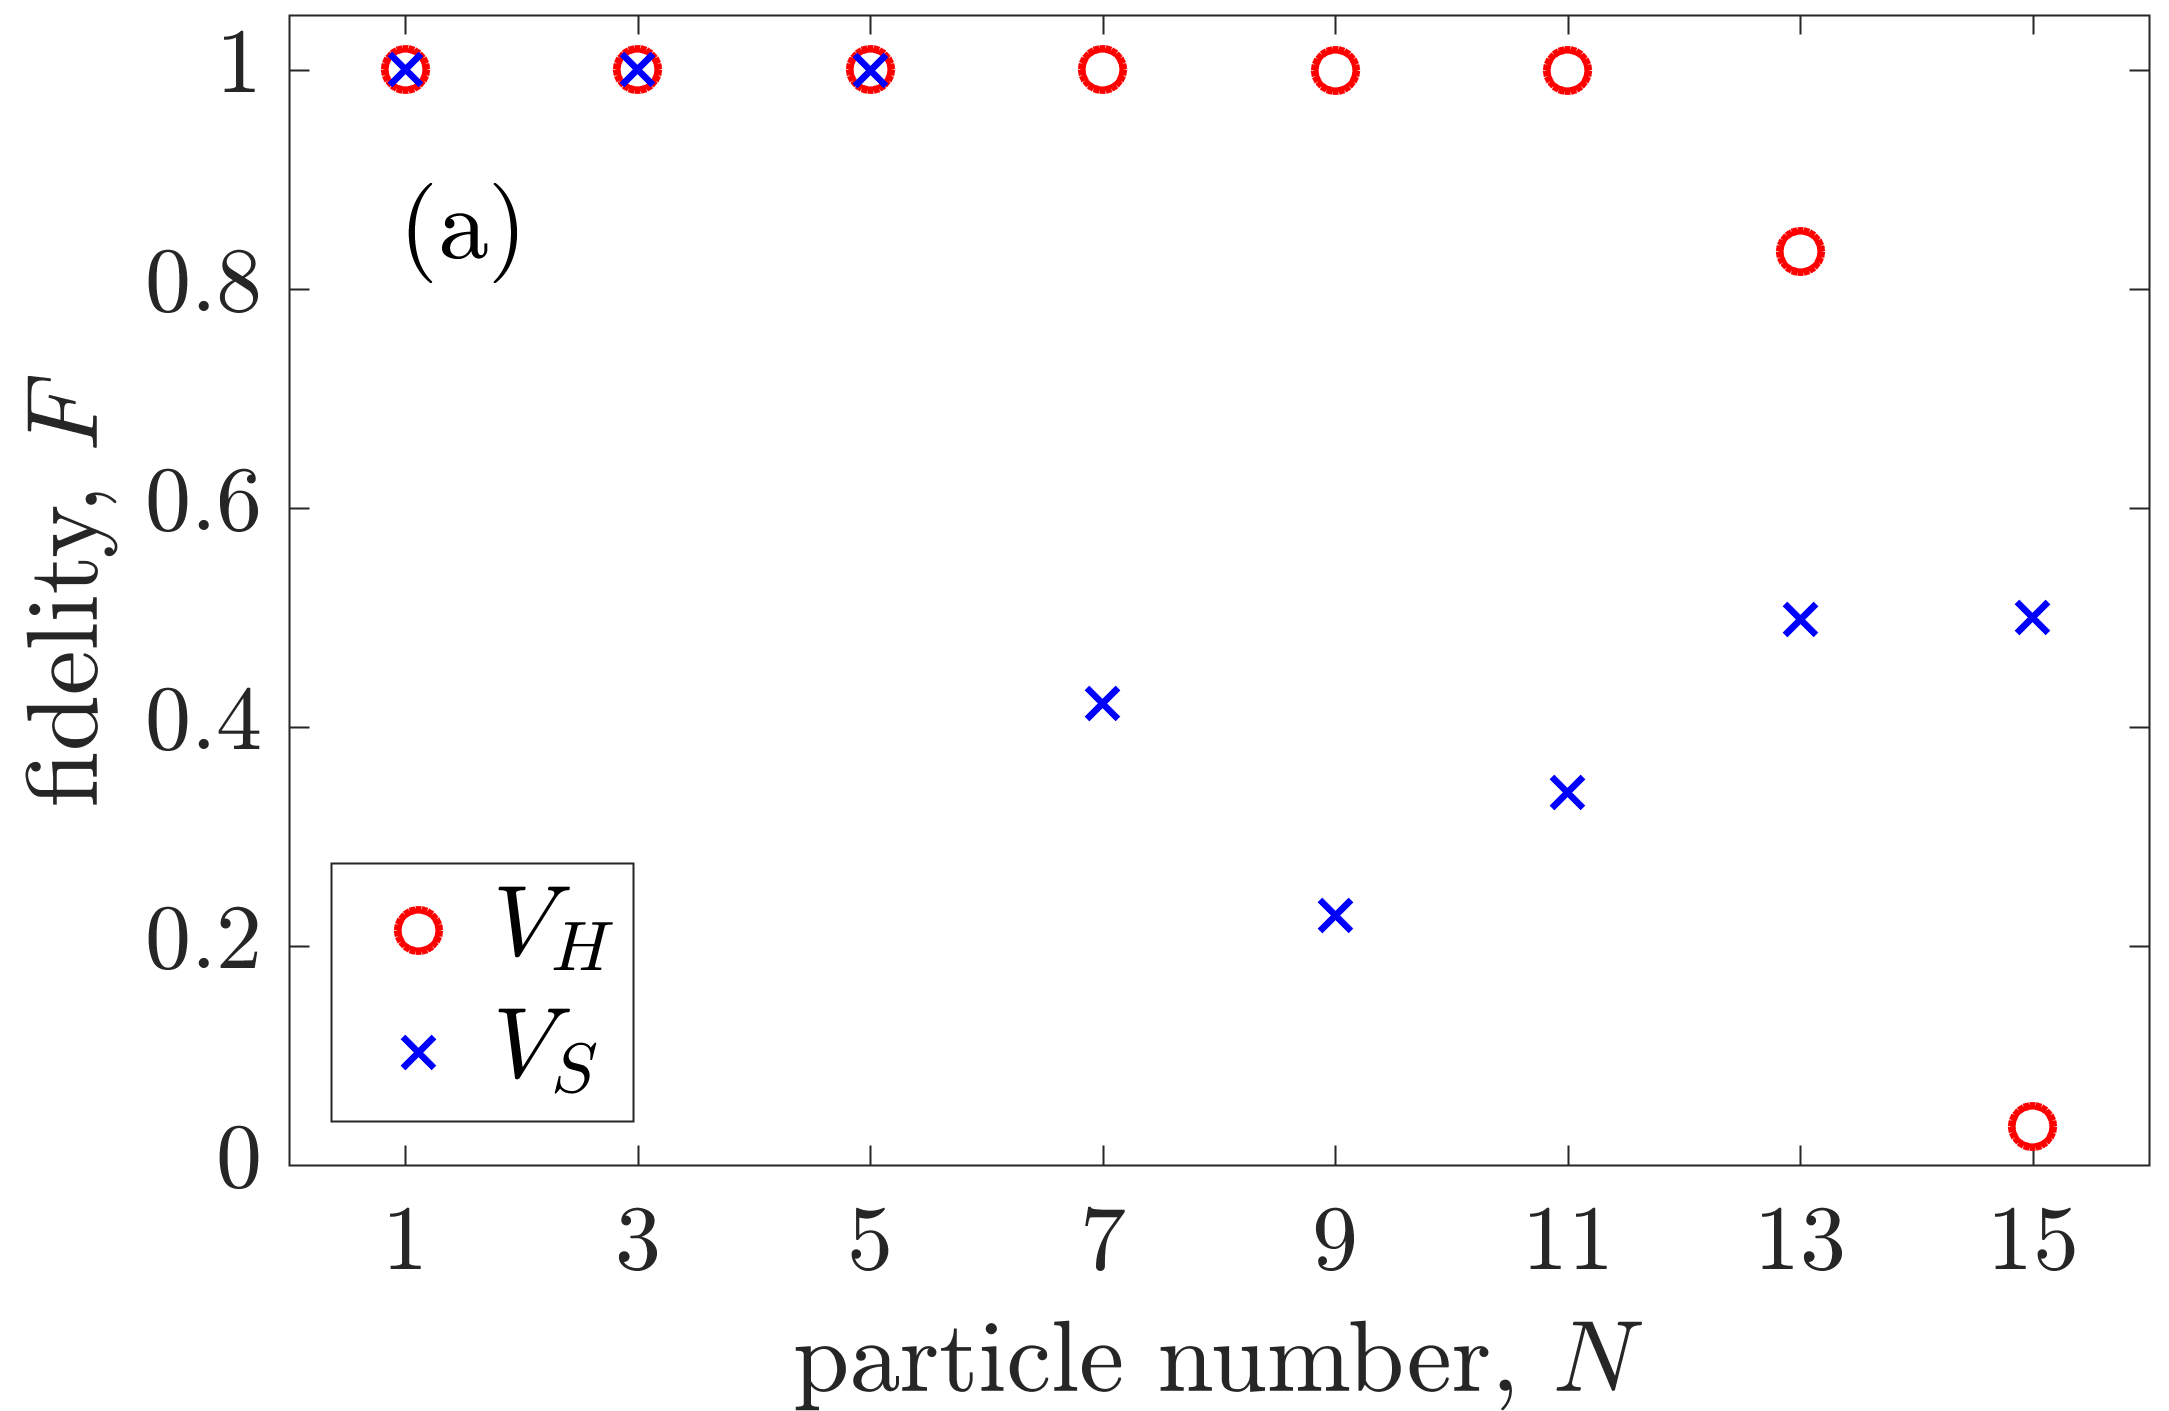
\includegraphics[width= 0.45\linewidth]{data/1d/fig7a.png} }
\subfigure{
\centering
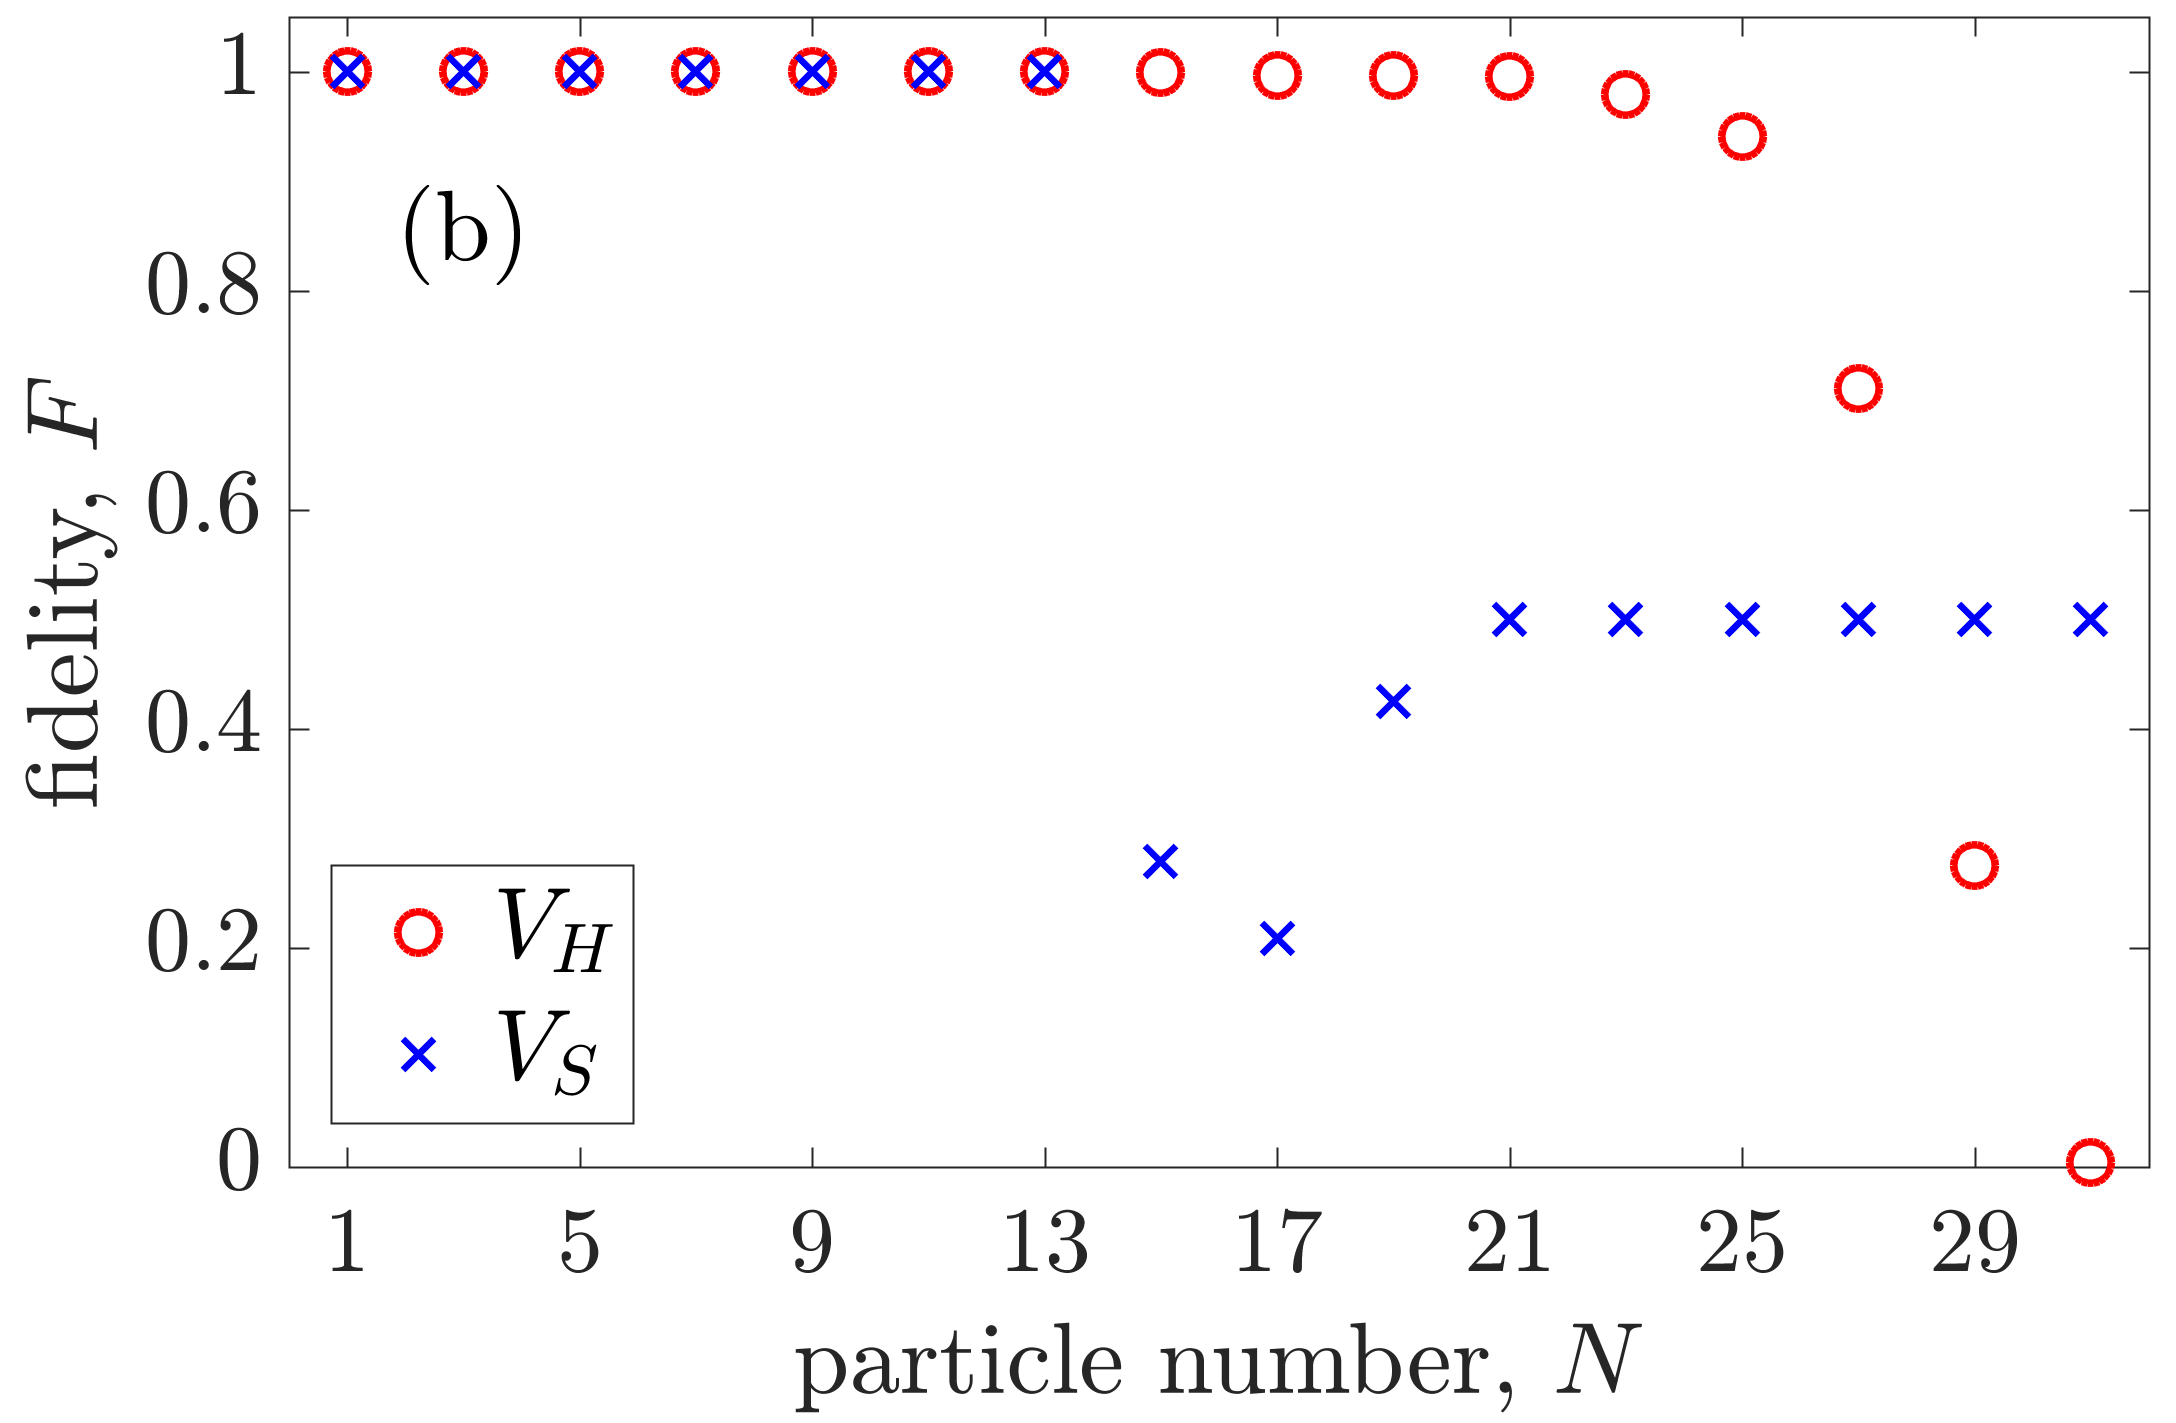
\includegraphics[width= 0.45\linewidth]{data/1d/fig7b.png}}
\caption{ Final fidelities $F$ of TG states of increasing particle number for the protocol shown in Figure \ref{fig:final+param}(a) with $\Omega_f = \pi$ for $V_H$ (red circle) and $V_S$ (blue cross). Plot (a) shows the fidelity of the protocol with $\omega_f = 100$ and (b) with $\omega_f = 200$.}
\label{fig:TG-STA}
\end{figure}

Any initial state $\ket{\phi^i_l}$ can be brought to the target state $\ket{\phi^t_l}$ with high fidelity with the proposed protocol, and the process also works for TG gases.
In Figure~\ref{fig:TG-STA}(a), the harmonic potential fidelities are shown to remain high for $N \leq 11$ after which they decrease due to a finite maximum height of the potential enforced by periodic boundary conditions.
The fidelities can be improved by increasing the maximum trapping frequency $\omega_f$ as was demonstrated in Figure \ref{fig:TG-STA}(b) where the value of $\omega_f$ is doubled and the fidelities remain high until $N \leq 21$.
When using the sinusoidal potential, the fidelity drops for smaller particle numbers compared to the  harmonic potential (although it also increases with $\omega_f$), due to the lower height $V_S$ has compared to $V_H$.

\section{Outlook}

In this chapter, quantum optimal control and STA protocols were introduced to optimize quantum engineering tasks in cold atomic gases.
I have introduced a physical system to generate NOON states in a TG gas non-adiabatically with both methods, and they were shown to be highly effective.
Such dynamical evolution techniques require time-dependent control parameters, such as rotation frequency or barrier height, and allowing for these dynamic operations has hitherto been a difficult task on GPU hardware.
In the following chapter, I will discuss GPU hardware in-depth and also tackle this issue, along with several others noted in Chapter~\ref{ch:splitop}.


\chapter{General Purpose computing with Graphics Processing Units and the GPUE codebase}
\label{ch:gpu}

The Graphics Processing Unit (GPU) is a computing card that typically connects to the motherboard through a Peripheral Component Interconnect (PCI) slot.
As the name implies, the GPU is designed to rapidly manipulate memory to create images or graphics that are sent to a display device, such as a monitor.
Because individual pixels in images are independent of each other and modern computers require updating all pixels on the display device quickly, the GPU has been developed as a massively parallel computing device, capable of efficiently performing simple tasks (such as pixel generation or manipulation) rapidly by distributing the computation among many computing cores.
This design methodology starkly contrasts the few, powerful cores on the Central Processing Unit (CPU), which is the default computing device on modern desktop systems.
Due to this difference in hardware design, there are also several optimizations to consider when programming for massively parallel GPU devices, and several of these techniques will be covered in this chapter.

As GPU technology grew, other areas of computational science became increasingly hungry for computing power, specifically in the area of scientific computing on High-Performance Computing (HPC) systems.
Historically, HPC systems were often developed as large, distributed networks of computing nodes intended for CPU-based computation.
As such, these systems facilitated the development of highly parallel and distributed numerical methods to perform scientific computation.

With new, parallel algorithms being developed for HPC systems and GPU technology advancing rapidly to perform more computation in parallel to satiate the consumer demands for high-quality videos and graphics for video games and other media, it became possible to use the GPU as a scientific computing device as well with a new technique called General Purpose computing on Graphics Processing Units (GPGPU).
Modern HPC design often incorporates the GPU into each computing node, thereby increasing the throughput of the system, overall, and the fastest known supercomputer today (Summit, ORNL~\cite{kahle2019}), is almost entirely composed of GPU nodes with NVIDIA Tesla V100 cards (32 GB of available RAM), connected with NVlink and IBM's power architecture.
In addition to the utility of GPGPU for scientific computing, GPU technology has also been rapidly developed for AI and related fields.

In this chapter, I will discuss the design methodology for the hardware and software related to GPGPU before proceeding to the development of GPUE, the GPU-based Gross-Pitaevskii Equation solver, which will be used for the remainder of this work.
To start, I will first look into different types of parallelism and how these affect different hardware and software practices.

\section{Types of parallelism}

Older CPU architecture with a single core was designed as SISD (Single Instruction, Single Data) according to Flynn's taxonomy~\cite{gurd1988}. 
This simply means that no parallelism exists in the instructions or data.
Even now, most code is na\"ively written as if it is to be executed on SISD architecture, even though it is rare to find such a system in modern environments.
For capable devices, there are two separate methods to parallelize computation: \textit{Task parallelism} and \textit{data parallelism}.

Task parallelism allows programmers to split their computation along separate, non-interacting \textit{tasks} or instructions, where each core performs its designated computation before moving on.
On the other hand, data parallelism allows programmers to perform the same, repetitive task along a large data set by distributing worker threads across the data.
Task parallelism is often better for dealing with a large number of specific actors, while data parallelism is often better for dealing with a large number of similar tasks on the same data, such as operations on a large matrix.
If a computing architecture allows for multiple instructions, but only a single data stream, it is considered to be MISD (Multiple Instruction, Single Data) by Flynn's taxonomy; meanwhile, if the architecture allows for multiple data streams with only a single instruction, it is considered to be SIMD (Single Instruction, Multiple Data).
Most modern HPC systems are designed to be MIMD (Multiple Instruction, Multiple Data), and both task and data parallelism is exploited by developers; however, for GPU computation, data parallelism is often used more frequently.

In the realm of data parallelism, there is an extreme case where the data is \textit{embarrassingly parallel}.
Here, there could be a large matrix of data to manipulate, but no single element depends on any other.
This means that when distributing computation along this matrix, we can simply assign tasks to each core without considering interactions with the rest of the data set.
In this way, it is embarrassingly easy to parallelize, and hence the term \textit{embarrassingly parallel}.
As a note, element-wise matrix multiplications are embarrassingly parallel operations; however, FFTs are not~\cite{czechowski2012}.
As such, the SSFM is not overall embarrassingly parallel; however, because the FFTs are handled by the CuFFT library, programmers do not often need to consider task parallelism at all when developing SSFM code.
Even so, understanding all the features of GPUE and its future directions requires a strong understanding of GPGPU, and this will be discussed in the following section.

\section{General purpose computing with graphics processing units}

GPGPU programming is a relatively new development to the computing world and is generally much faster than CPU-based computation for tasks that can be easily parallelized in a SIMD-like fashion.
Though benchmarks vary greatly depending programming languages, code quality, and intent of the software being benchmarked, our GPUE codebase is often 5 to 10 times faster than well-optimized C/C++ code and 100-200 times faster than Matlab code that is simulating the same system~\cite{wittek2016}.
This is shown in Figure~\ref{fig:bench}, where a comparison between GPUE, GPElab~\cite{antoine2014}, and Trotter-Suzuki~\cite{wittek2013} are shown.
These benchmarks are consistent with other GPGPU programs~\cite{garland2008, lee2010, nickolls2010}.

\begin{figure}
\center 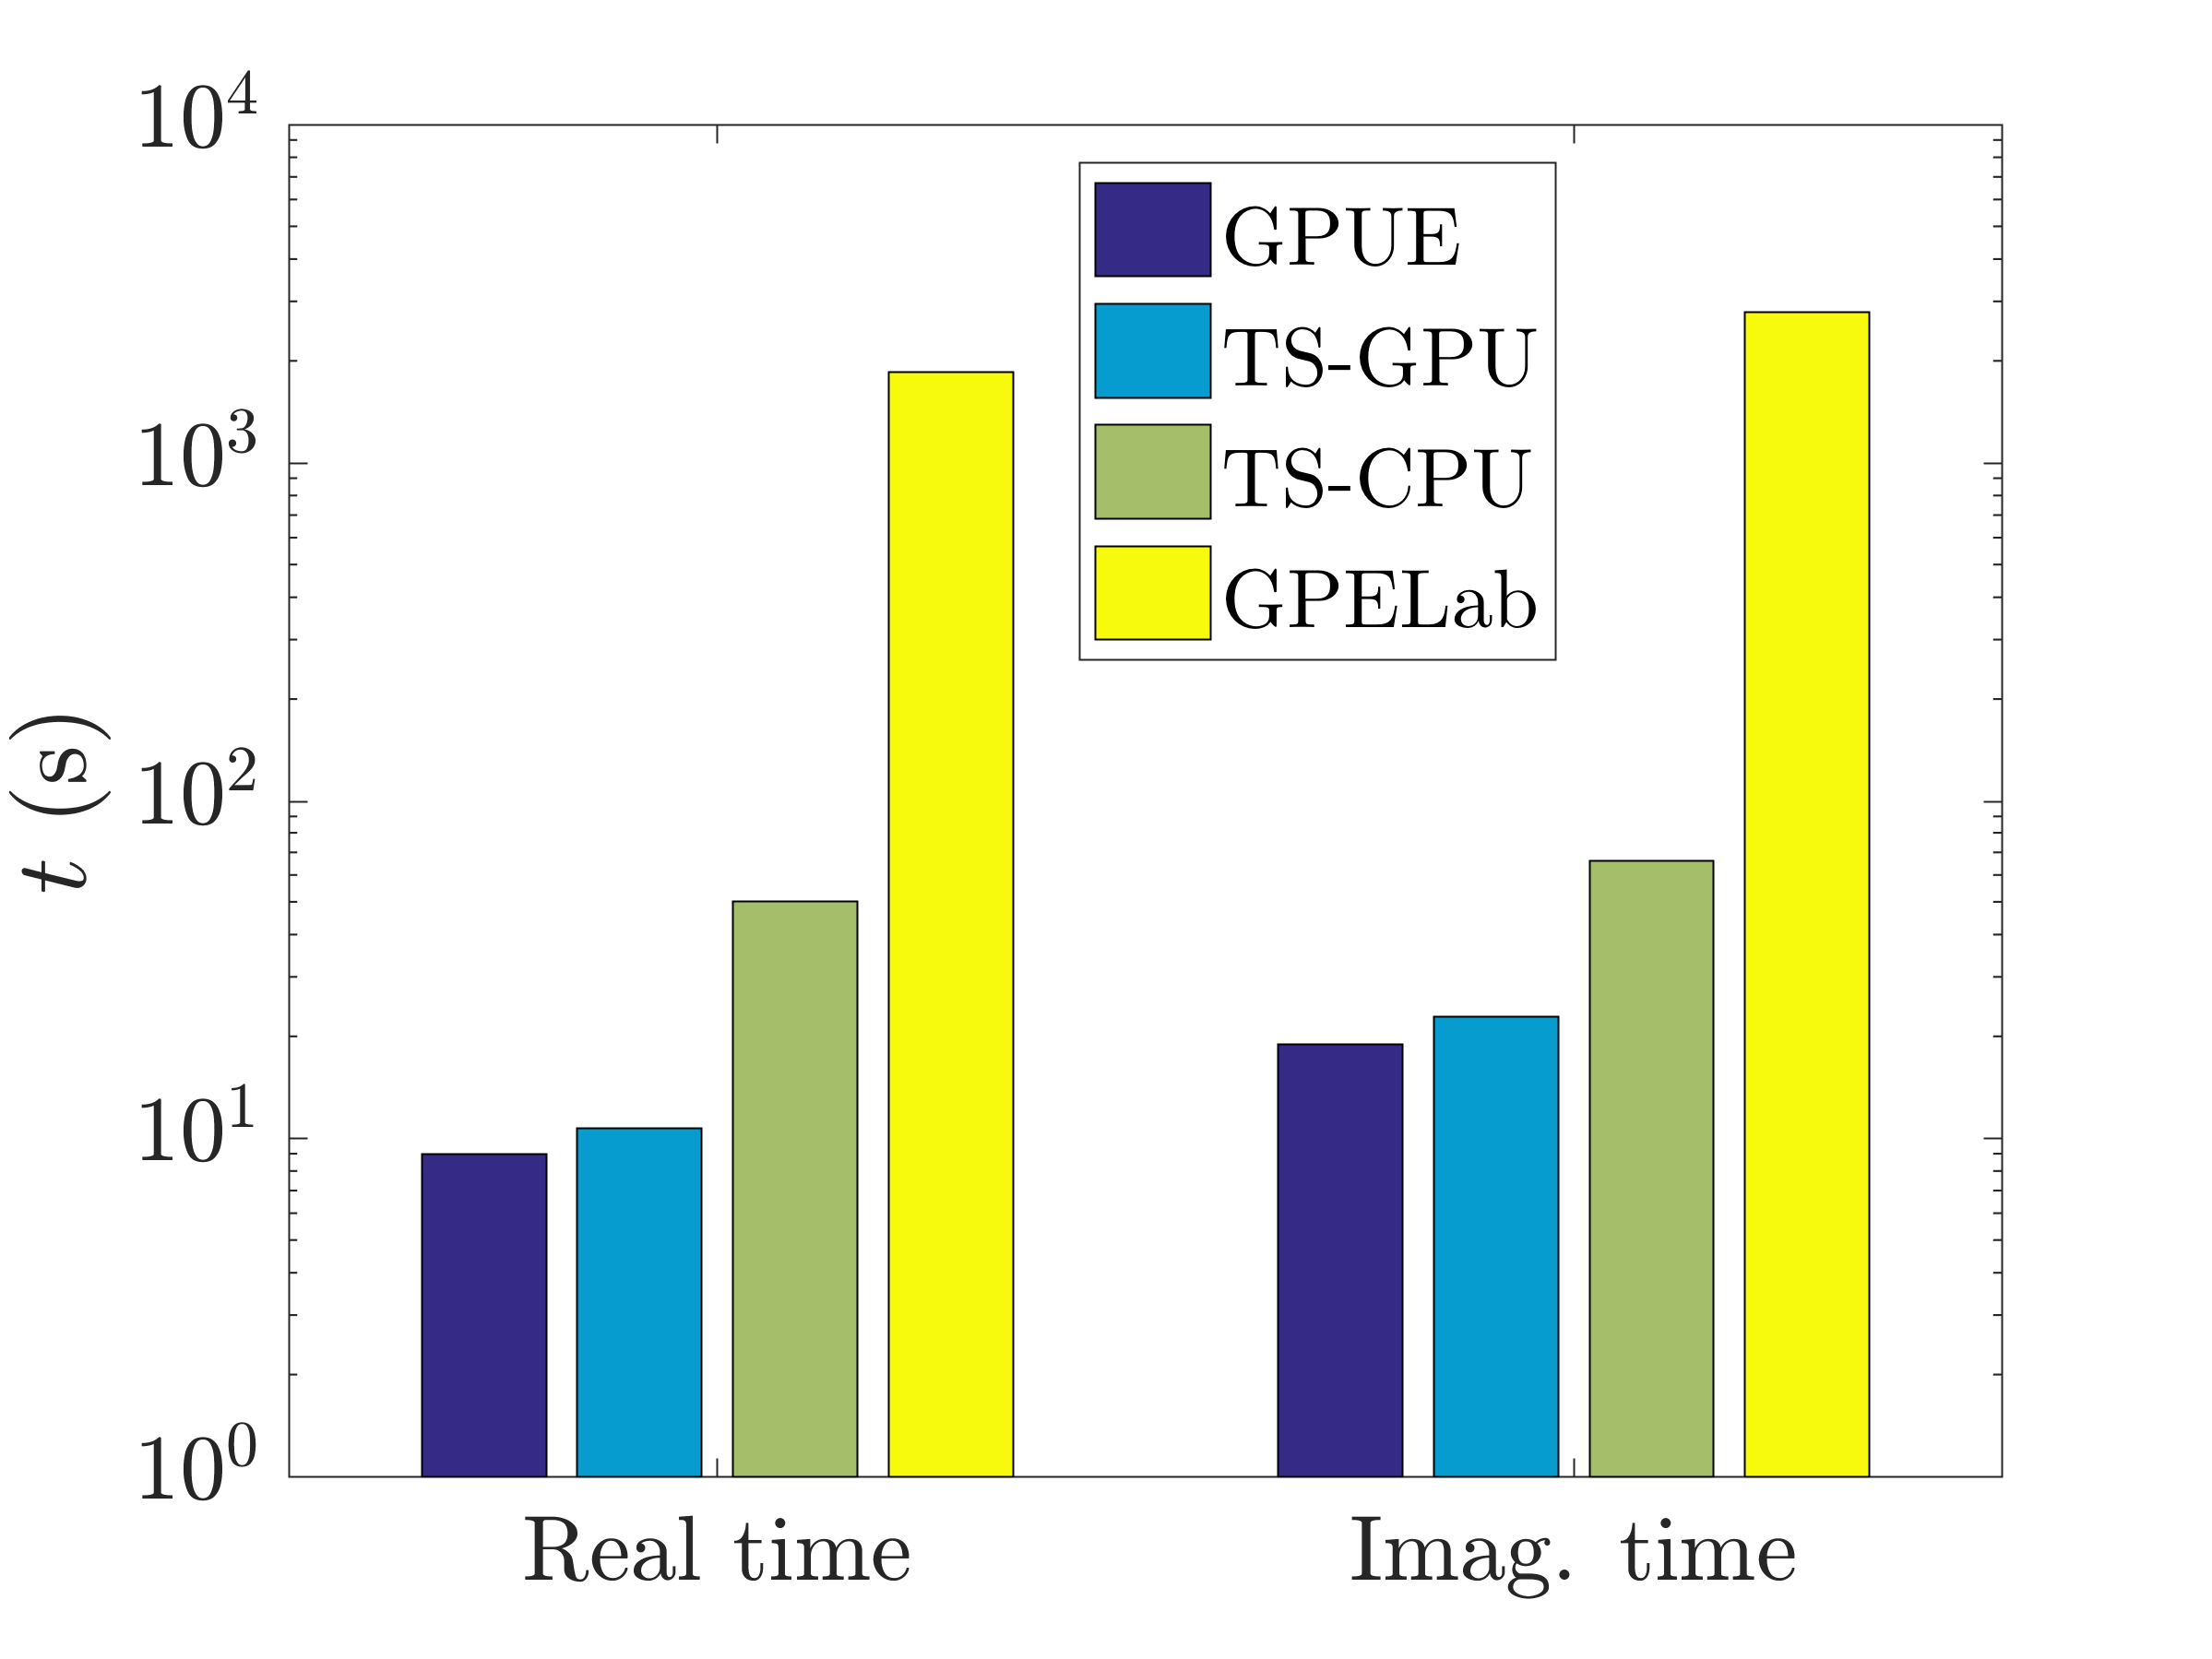
\includegraphics[width=0.5\textwidth]{data/gpu/GPUEvsTS.png}
\caption{Comparison between GPUE (CUDA), Trotter-Suzuki on both GPU (CUDA) and CPU (C++), and GPElab (Matlab).
Here, it is shown that GPUE is marginally faster than Trotter-Suzuki, but both GPU implementations are faster than the CPU-based variants.
Both software packages are much faster than GPElab.}
\label{fig:bench}
\end{figure}

As it is possible to massively increase the performance of certain programs by using GPU hardware, it is important to discuss the differences between GPGPU and CPU-based computation, along with important optimizations for GPU computing that will be used throughout this work.
For the remainder of this work, I will use the term \textit{host} interchangeably with CPU and \textit{device} with GPU.

\subsection{Limitations of GPU computing}

GPGPU and massively parallel computation are best suited for embarrassingly parallel systems and there are several problems that are poorly suited to parallelization.
For example, any task that is inherently iterative (such as summation) or recursive (such as tree traversal) is not suited for parallel computation.
Even so, there are methods to re-frame these problems such that they are better optimized for massively parallel devices, and these will be covered when relevant to the development of GPUE.

In addition to these algorithmic limitations, GPU cards have several notable drawbacks in terms of available memory on individual cards, which is often much less than the amount available on the host.
As such, when simulating a large system on the GPU, one often limits the resolution to what can fit onto GPU memory.
In addition the data transfer between GPUs and between the GPU and CPU through the PCI port is a slow process.
Until recently, these limited the size of the simulated wavefunction with GPUE to roughly $512^3$ on a single Tesla K80 card.
Higher resolution simulations could be performed with more recent cards (such as the Tesla V100) or by using multiple cards; however, because it takes time to transfer data between GPUs, it is preferred to use a single card where possible.
At this point, it is worthwhile to fully discuss GPU hardware and software ideologies, with particular focus on areas relevant to the development of GPUE.
We will discuss important methods used in the development of GPUE to overcome shortcomings in GPGPU afterward in Section~\ref{sec:GPUE}.

\subsection{GPU hardware architecture}

Even though several programming frameworks exist with the capability of running code on the GPU, most of these hide necessary optimizations from the user.
As such, I have chosen to focus exclusively on programming frameworks that expose the hardware for software developers, such as CUDA, OpenCL, and Julia.
Though the following discussion will primarily focus on CUDA, a brief discussion of OpenCL and Julia can be found in Section~\ref{sec:compare}, and example code for both languages can be found in the Appendix~\ref{app:GPU}.
For the purposes of this discussion, I will cover only the GPU memory architecture of NVIDIA GPU devices as these are the most common computing devices for HPC systems.

This topic is easiest to describe by dividing it into two parts: an introduction to the software interface as defined by the CUDA API, followed by a discussion of the memory and thread hierarchy of GPU devices.
Throughout these sections, I will discuss performance tips to ensure maximum GPU utilization, memory throughput, and instruction throughput.

\subsubsection{Introduction to CUDA software interface}

The CUDA parallel computing platform bares the hardware of the GPU to software developers.
This means that important elements of this programming interface will appear in subsequent sections regarding hardware limitations and performance guidelines.
Much of this discussion can be found in the \textit{CUDA C Programming Guide}~\cite{CUDAPG}, while other sources will be cited as necessary.
Full code for this discussion can be found in the Appendix~\ref{app:GPU}.

\begin{lstlisting}[float,label=lst:vecadd,caption={An example of vector addition performed in C or C++ for $a$, $b$, and $c$, all of size $n$},style=c++]
for (int i = 0; i < n; ++i){
    c[i] = a[i] + b[i];
}
\end{lstlisting}

I will show a simple example where we would like to add two vectors such that $\mathbf{a} + \mathbf{b} = \mathbf{c}$.
This can be done with a simple loop in C, shown in Listing~\ref{lst:vecadd}.
In this case, we take each element with a specified ID in $\mathbf{a}$ and $\mathbf{b}$ and add them to the appropriate ID $\mathbf{c}$.
In some parallel programming models (OpenACC~\cite{wienke2012}, OpenMP~\cite{chandra2001}, GPUifyLoops.jl, and many others), parallelization of this method is possible by adding a macro to the start of the loop to specify that the operation is to be performed in parallel; however, this obscures GPU hardware for the user and does not always have the same performance guarantees~\cite{reyes2012}.
As such, CUDA takes a slightly different approach by encouraging software developers to write \textit{kernels}, specific to the computation at hand.
An example CUDA kernel for vector addition is shown in Listing~\ref{lst:vecaddCUDA}, which has a number of notable differences to the loop in C in Listing~\ref{lst:vecaddCUDA}.
This kernel is already remarkably different than an expected function on the CPU, and it is worth comparing Listings~\ref{lst:vecadd} and \ref{lst:vecaddCUDA} in detail for a better understanding of GPU hardware.

\begin{lstlisting}[float,label=lst:vecaddCUDA, style=c++,caption=An example of a vector addition kernel in CUDA]
__global__ void vecAdd(double *a, double *b, double *c){

    // Global Thread ID
    int id = threadIdx.x;

    c[id] = a[id] + b[id];
}
\end{lstlisting}

The first peculiarity appears in line 1 with the \texttt{\_\_global\_\_} function specifier.
This is a necessary element of all CUDA kernels that specifies where and when this kernel is capable of being called.
A \texttt{\_\_global\_\_} kernel can be called by either host (with a standard CPU function) or the device (with a GPU kernel).
A \texttt{\_\_host\_\_} kernel is exactly the same as a CPU function and can only be called by other CPU functions.
Finally, a \texttt{\_\_device\_\_} kernel can only be called by other \texttt{\_\_device\_\_} or \texttt{\_\_global\_\_} kernels.
As a note \texttt{\_\_global\_\_} kernels are incapable of returning vectors or other variables, and must instead mutate the variables, themselves.
This is why the \texttt{\_\_global\_\_} \texttt{vecAdd(...)} kernel does not return $c$, but instead assumes it is a pre-allocated variable.

Another peculiarity appears on line 6, where the addition, itself, occurs.
Though there was a necessity for a loop in Listing~\ref{lst:vecadd}, there does not seem to be one at all in Listing~\ref{lst:vecaddCUDA}.
This is because the GPU is performing this task in parallel and handling the parallelism behind the scenes on line 4 with the \texttt{int id = threadIdx.x} command.
In this line, we are identifying which element of the array we are operating on with the CUDA-specific \texttt{threadIdx.x} variable.

Here, each \textit{thread} is an individual instructional element acted on in parallel with other threads in the same \textit{block}, which is further subdivided into \textit{grids}.
All threads in the same block have a \textit{shared memory} resource, while all three structures have access to \textit{global memory}.
In general, it is important to use shared memory when possible, as it has a lower latency than global memory, and this will be discussed further in subsequent sections.
As a note, threads often work without feedback from other threads; moreover, it may be necessary to stop thread execution until all other threads have caught up.
This can be done with the \texttt{\_\_syncthreads()} function in CUDA.

Threads, blocks, and grids are all \texttt{dim3} variables with $x$, $y$, and $z$ attributes.
The way in which these threads and blocks are allocated are defined by the user before kernel execution.
Often times, a thread number of 1024 is chosen, and the number of blocks is decided based on the size of the input array.
If there are more elements to compute than threads in a block, one then need to use the \texttt{blockDim.x} and \texttt{blockIdx.x} variables to access the appropriate threads for computation.
All threads are indexed as one-dimensional vectors even in a multidimensional space, as shown in Figure~\ref{fig:threadsnblocks}.
Even though threads are rarely acted on sequentially, the thread ID has important ramifications that will be discussed further with other performance tips.

\begin{figure}
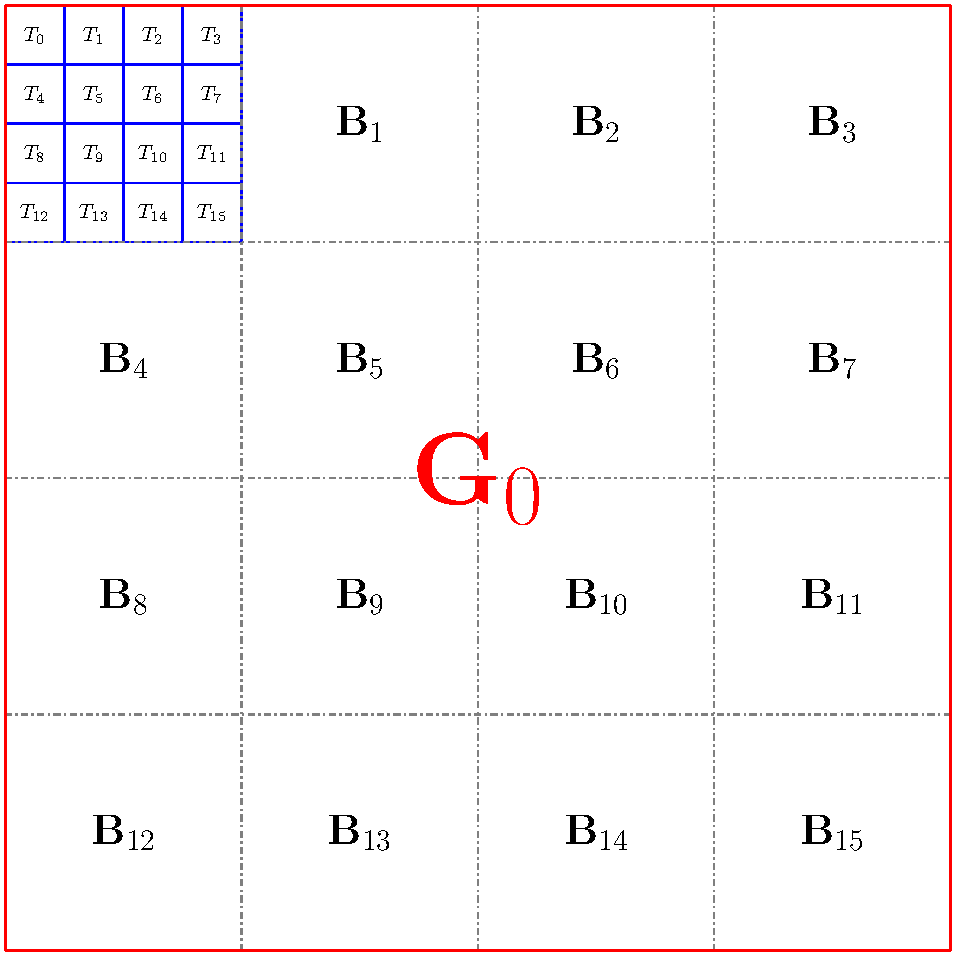
\includegraphics[width=\textwidth]{data/gpu/gputhreads.pdf}
\caption{Each grid is subdivided into multiple blocks, which is further subdivided into threads for computation. Each thread has a specified ID, which acts as a one-dimensional array, even in a two or three-dimensional system. Here, all areas outlined in red have access to global memory, and any area outlined in blue has access to shared memory. \jrs{slight modification necessary to show 1D indexing!}}
\label{fig:threadsnblocks}
\end{figure}

As another note, CUDA will execute code on unallocated memory if one does not tell it to otherwise.
As such, if one had failed to set the number of threads in the block to the number of elements in the array in Listing~\ref{lst:vecaddCUDA}, the kernel would exhibit undefined behavior.
For this reason, one needs to take into account potential out-of-bounds computation.
If one takes the above example of vector addition, assuming that the thread count is higher than can fit in one block and take into consideration potential out-of-bounds behavior, the kernel would instead look like Listing~\ref{lst:vecaddCUDA2}.

\begin{lstlisting}[float,label=lst:vecaddCUDA2, style=c++,caption={An example of a vector addition kernel in CUDA using blocks and threads, and ensuring no computation happens beyond the size of the array, $n$.}]
__global__ void vecAdd(double *a, double *b, double *c, int n){

    // Global Thread ID
    int id = blockDim.x * blockIdx.x + threadIdx.x;

    if (id < n){
        c[id] = a[id] + b[id];
    }
}
\end{lstlisting}

Finally, I need to discuss how software developers call these CUDA kernels in host code.
This requires the developer to allocate space on the device for use in the CUDA kernel via a \texttt{cudaMalloc(...)} command.
Often times, arrays on the host must also be established and transferred to the device with \texttt{cudaMemcpy(...)} functions as well.
In addition, the kernel must be configured before running with \lstinline{<<<grid, threads,...>>>}.
When everything is considered, the host code might look like what is shown in Listing~\ref{lst:vecaddhost}

\begin{lstlisting}[float,label=lst:vecaddhost, style=c++,caption={An example of host code to run Listing~\ref{lst:vecaddCUDA2}.}]
int main(){

    int n = 1024;

    // Initializing host vectors
    double *a, *b, *c;
    a = (double*)malloc(sizeof(double)*n);
    b = (double*)malloc(sizeof(double)*n);
    c = (double*)malloc(sizeof(double)*n);

    // Initializing all device vectors
    double *d_a, *d_b, *d_c;

    cudaMalloc(&d_a, sizeof(double)*n);
    cudaMalloc(&d_b, sizeof(double)*n);
    cudaMalloc(&d_c, sizeof(double)*n);

    // Initializing a and b
    for (size_t i = 0; i < n; ++i){
        a[i] = i;
        b[i] = i;
        c[i] = 0;
    }

    cudaMemcpy(d_a, a, sizeof(double)*n, cudaMemcpyHostToDevice);
    cudaMemcpy(d_b, b, sizeof(double)*n, cudaMemcpyHostToDevice);

    dim3 threads, grid;

    // threads are arbitrarily chosen
    threads = {100, 1, 1};
    grid = {(unsigned int)ceil((float)n/threads.x), 1, 1};
    vecAdd<<<grid, threads>>>(d_a, d_b, d_c, n);

    // Copying back to host
    cudaMemcpy(c, d_c, sizeof(double)*n, cudaMemcpyDeviceToHost);

    // Check to make sure everything works
    for (size_t i = 0; i < n; ++i){
        if (c[i] != a[i] + b[i]){
            std::cout << "Yo. You failed. What a loser! Ha\n";
            exit(1);
        }
    }

    std::cout << "You passed the test, congratulations!\n";

    free(a);
    free(b);
    free(c);

    cudaFree(d_a);
    cudaFree(d_b);
    cudaFree(d_c);
}
\end{lstlisting}

All said, vector addition is often known as the ``Hello World!'' of GPU programming as it is the first application that shows the parallelism of GPU devices; however, even here, a distinction between users and developers can be seen.
As more complex software is developed, it becomes more important to write software in such a way that users do not directly interface with CUDA code, and the full ramifications of this will be discussed in later in this chapter.
In addition, this discussion highlights the important distinction between host and device code, including the concept of threads and blocks, shared memory, and the ability to transfer data from the host to the device, all of which are essential to understanding particular design decisions of GPUE.
For now, I will continue this discussion by moving to GPU hardware, focusing on thread and memory hierarchy.

\subsubsection{Discussion of GPU thread and memory hierarchy}

Every time host code invokes a CUDA kernel call (as shown in Listing~\ref{lst:vecaddhost}), the data is mapped to a scalable array of multiprocessors on GPU hardware.
Multiple blocks might be distributed to the same multiprocessor, but blocks are always distributed contiguously.
Each multiprocessor is designed to execute hundreds of threads in parallel by using a unique SIMT (Single Instruction, Multiple Threads) architecture, which is similar to SIMD and can be used as such for most cases; however, there are performance benefits to optimizing instruction-level parallelism at the thread level.
Each multiprocessor distributes its parallel processes into \textit{warps}, which are units of 32 threads that execute a single common operation at a time.
Notably, the way a block is distributed into warps is always the same, so it is important to ensure that the input data is in powers of 32 to avoid wasting unnecessary computation.
Outside of this, developers can often ignore SIMT behavior as long as they do not allow threads in a warp to have separate operations.

Understanding GPU memory architecture is essential to properly using GPU hardware, and as such, it is worth discussing in-detail.
There are three forms of GPU memory that are useful for most applications of GPGPU for scientific computation: global memory, shared memory, and texture memory.
As described above, global memory is shared between all grids, blocks, and threads and is considered to be the slowest memory bank.
As such, whenever a warp accesses global memory, it tries to perform as few accessing operations as possible, which is made easier if the warp needs to access contiguous memory blocks.
If the warp is required to access non-contiguous blocks, more accesses will be necessary and thus performance will take a relatively large hit.
For this reason, it is important to make sure all data accesses are \textit{coalesced}, which ensures that the warp will access consecutive elements as depicted in Figure~\ref{fig:threadsnblocks}.

For optimal memory throughput, shared memory is an essential tool to understand and use appropriately.
As described, shared memory is on-chip memory that is shared between all threads in a block.
The amount of shared memory available is hardware-dependent and configurable on kernel execution.
In general, it is worthwhile to transfer data with a large number of accesses to shared memory for performance.
Shared memory is split into several memory banks which can be accessed simultaneously.
If two memory accesses are required of the same bank, there will be a conflict (known as a bank conflict) and the operation can no longer be performed in parallel.
It is sometimes necessary to pad variables to prevent bank conflicts from occurring~\cite{harris2013}.

Of the three types of memory mentioned, texture memory is the least-often used and is primarily on the GPU for graphics computation and focuses on performance for two-dimensional structures.
Texture memory has a relatively long write time, but is quick to read.
It is also faster than global memory for non-coalesced access patterns and therefore can be useful for certain tasks with slowly varying operators.
In principle, this is the case for the momentum-space operator in the SSFM; however, because texture memory uses single-precision, it will not be used further in this work.

In addition to appropriate usage of memory on GPU architecture, it is also essential to minimize data transfers between the device and host and even between devices in multi-GPU setups.
The data transfer between the host and device or between devices must send data through the PCI slot on the motherboard, which is a slow operation.
For data transfer between devices, this transfer time can be slightly alleviated on Power architecture where NVlink technology can directly transfer data from device to device~\cite{foley2017}, but the data transfer between devices will still likely be the slowest part of the computation.
In addition, CUDA-aware MPI for multi-GPU setups may add an huge burden on software development time~\cite{lonvcar2016, wang2013}.
As such, developers often try to keep all of their computation on a single card, if possible, and several optimization strategies are used when multiple GPU cards are needed.
These strategies will be covered on a case-by-case basis as they arise in this work.

As a final note, one optimization strategy for CUDA code that will not be discussed in-depth in this work is the maximization of instruction throughput.
The simplest optimizations here involve increasing the number of instructions performed over a specified period by trading precision for speed and minimizing thread synchronization.
Because we are performing high-precision superfluid simulations, we cannot perform a trade-off between precision and computational speed.
When optimizing the instruction throughput for GPU devices, it is important to discuss conditionals, like \texttt{if} and \texttt{switch} statements.
Here, programmers need to be careful not to accidentally cause the operation executed on threads in a warp to diverge.

\subsection{Comparison between various languages for GPGPU computation}
\label{sec:compare}

As one might expect, specialized programming languages are necessary to write code that compiles and runs on GPU architecture.
There are several known libraries to extend modern programming languages such as Matlab, python, and C++ to GPU devices; however, we will limit this discussion to common programming methods that allow fine-grained control of GPU memory and could be used for the development of GPUE.
We will briefly discuss the advantages and disadvantages of three competing languages considered here: CUDA, OpenCL, and Julia, and as a simple example, vector addition in these languages is shown in  Appendix~\ref{app:GPU}.

\subsubsection{CUDA}
CUDA is a computing API provided by NVIDIA for interfacing with NVIDIA GPUs and is the industry standard for GPGPU programming.
CUDA is primarily limited by the NVIDIA-specific hardware it runs on, and although NVIDIA currently produces the most common GPUs for GPGPU programming, AMD GPU devices are also available and often cheaper for a similar level of computational power.
In addition, CUDA support has recently ceased for MacOS systems as NVIDIA cards are no longer bundled with current generation Mac computers, so CUDA code can only be used on Windows and Linux devices with NVIDIA cards.
GPUE was written entirely in CUDA; however, due to the aforementioned limitations, there has been some consideration to re-writing the software in OpenCL or Julia.

\subsubsection{OpenCL}

Though CUDA is the industry-standard for GPGPU programming, OpenCL (Open Compute Language) is largely competitive in terms of performance and has the benefit of being compatible with both NVIDIA and AMD GPU devices.
OpenCL is also completely open-source and works as additional libraries to C or C++, which allows developers to compile OpenCL code with traditional compilers like \texttt{gcc} or \texttt{clang}.
OpenCL has nearly similar structure to CUDA with slightly more verbose syntax, and thus provides all necessary functionality to develop and maintain scientific software.
It should be mentioned that OpenCL also has the capability of running on a large variety of other computing architectures, such as FPGA and is a more general-purpose computing library than CUDA.
In addition, compute kernels are compiled at run-time, meaning that users can potentially modify kernels without recompiling the code.
This could be a huge boon for developers writing software for users who may need to quickly simulate a slightly modified system.
Unfortunately, OpenCL has a rather cumbersome interface and has less support than CUDA for GPGPU.
As such, it is not often used for scientific computing software.

In the end, although OpenCL does provide the ability to more easily construct dynamic kernels, the increased engineering time necessary to write software in OpenCL is often not worth the cost; however, further advances in compiler design for heterogeneous architecture has been made in the past few years \cite{besard2019}, which has provided the unique opportunity for computer scientists to write maintainable and fast code in new languages, like Julia.

\subsubsection{Julia}
Julia is a new language to scientific computing, but boasts promising results.
It claims to be as usable as Python, but as performant as C~\cite{bezanson2017}, which is a huge boon for maintainability of HPC software.
In addition, Julia's runtime is comparable to CUDA C for GPGPU computation and allows for similar hardware optimizations \cite{besard2016, besard2018}, while also allowing users to edit the compiler implementations at will.
This is an important point that will be discussed in more detail in Section~\ref{sec:expr_trees}.

In addition, because Julia is much easier to write than C for new programmers, GPU-based Julia code could allow developers to provide fast, efficient code with a usable interface for scientists and engineers.
The trade off between performance and readability in programming has been described as the ``two-language'' problem, as most scientific computing solutions to this point have required using two languages: a fast language for the back-end and a readable language for the user interface.
Julia succeeds in bridging the gap between the languages, effectively solving the two-language problem and allowing scientists and engineers to write efficient code that is also compilable on the GPU.
For these reasons, we have begun porting our CUDA code to Julia, as it will lead to simpler and more maintainable code in the future.
This will be further discussed in the outlook of this work, Chapter~\ref{ch:conclusion}.
In Chapters~\ref{ch:2d} and \ref{ch:vortex_states}, I will also introduce systems that could benefit from a Julia interface.

\section{Introduction to the GPUE codebase for $n$-dimensional simulations of quantum systems on the GPU}
\label{sec:GPUE}

At this point, all the motivation and background necessary has been provided to discuss GPUE, the GPU-based Gross-Pitaevskii Equation solver.
This codebase will be used for all remaining simulations performed in this work and its development has also inspired the development of other computational libraries such as the \texttt{DistributedTranspose.jl} package, which will also be discussed in Section~\ref{sec:DT}.
Some additional information on prior development of GPUE can be found in other sources~\cite{o2017}.
The GPUE codebase was published in the Journal of Open Source Software in 2018~\cite{schloss2018} and
was originally designed by Lee O'riordan with the capability of simulating large-scale Abrikosov lattices in superfluid BECs.
My focus with GPUE development has been to simulate three-dimensional systems and optimize the software for dynamic studies on GPU hardware.
For this section, I will first describe the FFT optimizations used in GPUE for three-dimensional simulations, followed by additional features necessary for dynamic simulations on GPU architecture.

\subsection{FFT optimization}

As mentioned in Chapter~\ref{ch:splitop} and previously in this chapter, the SSFM is primarily limited by the complexity of the FFT operations.
For a three dimensional simulation with gauge fields in the $\hat x$, $\hat y$, and $\hat z$ directions, one set of global FFTs and three sets of one-dimensional FFTs must be performed.
This is equivalent to two three-dimensional FFT operations, which become much undesirable when scaling to multiple GPU devices~\cite{czechowski2012}.
The CuFFT API provides an option for computing FFT's on separate batches of an array in GPU memory with the \texttt{cufftPlanMany(...)} command; however, if this command is repurposed for one-dimensional FFT operations, it does not provide the necessary functionality for FFTs across the $\hat y$ or $\hat z$ dimensions.
With the CuFFT library, all FFT operations performed with this plan must follow an indexing pattern, such that 

\begin{lstlisting}
input[b*idist + x*istride]
output[b*odist + x*ostride]
\end{lstlisting}

\noindent where \texttt{b} is the batch ID, \texttt{x} is the element ID, \texttt{idist} and \texttt{odist} are the distances between batches for the input and output array, respectively, and \texttt{istride} and \texttt{ostride} are the strides between consecutive elements for computation with the input and output array, respectively.
On the other hand, if data is transferred to the GPU, it is often re-indexed as a one-dimensional array, such that

\begin{lstlisting}
array[i,j,k] = array[i + j*xDim + k*xDim*yDim]
\end{lstlisting}

\noindent where \texttt{i}, \texttt{j}, and \texttt{k} are iterable variables in the $\hat x$, $\hat y$, and $\hat z$ directions, and \texttt{xDim}, \texttt{yDim}, and \texttt{zDim} are the dimensions in $\hat x$, $\hat y$, and $\hat z$, respectively.
As such, it is not possible to use the \texttt{cufftPlanMany} functionality to perform one-dimensional FFTs in $\hat y$ and $\hat z$; however, if we increase the number of batches to \texttt{xDim*yDim*zDim}, set the distance between each stride to 1, and assume the stride between each element is \texttt{xDim*yDim}, we can recreate the functionality of the FFT in the $\hat z$ direction.
For the $\hat y$ FFT operations, we need an external loop that iterates over each $xy$ slab, performing \texttt{xDim} operations on each slab, and this greatly hampers performance.

\jrs{Will add image, if time permits.}

With this considered, only one-third of the necessary FFT operations are appropriately coalesced in memory for three dimensional simulations.
Because FFTs are global operations that are best performed on contiguous chunks of memory, multi-GPU simulations with the SSFM are even less optimal.
This has motivated the development of other packages to allow for memory coalescence with FFT operations, such as the distributed transpose, which will be described in Section~\ref{sec:DT}.
Even though the three-dimensional FFT operations are the biggest bottleneck in the GPUE codebase, it is not easy to avoid usage of the \texttt{cufftPlanMany(...)} operation while still using CUDA.
This is why optimizations to GPUE FFT operations will be performed exclusively in GPUE.jl.
Next, I will focus on another feature that was inhibited by the CUDA framework, but is nevertheless possible: methods to enable dynamic quantum engineering with expression trees.

\subsection{Dynamic field input and output in GPUE with expression trees}

\label{sec:expr_trees}
As mentioned in Chapter~\ref{ch:1d}, quantum engineering typically requires some form of time-dependent variables, along with evolution in real time.
This means that the user must be able to input a time-dependent equation to GPUE, often for $V(t)$, $g(t)$, or $\mathbf{A}(t)$.
Because GPUE is written in CUDA, there is no straightforward method for the user to input time-dependent fields without recompiling the source code and modifying CUDA kernels at will, which is unnecessarily cumbersome for the user.
As such, we have provided a method for users to input the fields of their choosing as strings, which will be compiled into a set of operations to perform on the GPU through expression trees, which are similar to Abstract Syntax Trees (ASTs) in compiler design~\cite{cohen1991, reyes2011}.

\begin{figure}
\center %\documentclass{article}
%\usepackage{tikz}
\usetikzlibrary{arrows}
\tikzset{
  exprnode/.style = {align=center, inner sep=0pt, text centered,
    circle, draw=black, text width=1.5em},
  varnode/.style = {exprnode, red, draw=red},
  posnode/.style = {exprnode, green!50!black, draw=green!50!black},
  oprnode/.style = {rectangle, white, draw = blue, fill=blue},
}
%\begin{document}
  $V = \frac{1}{2}m\omega^2 x^2 t$
  
  \begin{tikzpicture}[->,>=stealth',level/.style={sibling distance = 5cm/#1,
    level distance = 1.5cm}]
    \node [oprnode] {$\cdot$}
      child{ node [oprnode] {$\cdot$}
        child{ node [oprnode] {$\cdot$}
          child{ node [exprnode] {$0.5$}}
          child{ node [exprnode] {$m$}}
        }
        child{ node [varnode] {$t$}}
      }
      child{ node [oprnode] {$\cdot$}
        child{ node [oprnode] {$\cdot$}
          child{ node [exprnode] {$\omega$}}
          child{ node [exprnode] {$\omega$}}
        }
        child{ node [oprnode] {$\cdot$}
          child{ node [posnode] {$x$}}
          child{ node [posnode] {$x$}}
        }
      };
  \end{tikzpicture}
%\end{document}

\caption{
Example of expression tree for $V=\frac{1}{2}m \omega^2 x^2 t$.
Blue, filled nodes are operations, leaf nodes are variables, time has been highlighted in red, and spatially-dependent variables are in green.
This visualization was modified from a form provided by Xadisten during a Twitch livestream.
}
\label{fig:expr_tree}
\end{figure}

An example of an expression tree can be seen in Figure~\ref{fig:expr_tree}.
These are evaluated depth-first to follow the traditional order of operations.
With this method, a user can type in a string, like \texttt{"V = m*omega*omega*x*x*t"}, and this will be parsed into a set of operations to be performed on-the-fly by the GPU.
After parsing user-provided equations, certain leaf nodes are designated as either spatially or temporally dynamic.
In the case of spatially dynamic variables (\texttt{x}, \texttt{y}, and \texttt{z}), values are taken from constituent vectors based on their \texttt{threadIdx.xyz} values, and for any equation that is dependent on \texttt{t}, a stored \texttt{time} variable is used.
This operation necessitates the usage of a dictionary data structure to hold all variables on the host in some fashion, which inhibits host performance; however, because the bulk of the computation is performed on the GPU, this does not significantly impact GPUE performance, overall.
On the GPU, each necessary variable can be stored in a shared memory buffer, and even though we are replacing the embarrassingly parallel element-wise matrix multiplications with these expression trees, the performance is not severely impacted; however,
because parsing expression trees is an inherently iterative process, the longer the expression, the less optimal using this method is.
Ultimately, more work could be done in the future to maximize instruction throughput with our implementation of GPU-accelerated expression trees.

Not only do expression trees allow for STA and quantum optimal control methods to be used with GPUE, but they also eliminate the need to store any operators in GPU memory, effectively increasing the available memory by a factor of 5 for each three-dimensional simulation, as $V$, $K$, $A_x$, $A_y$, and $A_z$ no longer need to be stored.
This allows one to perform higher-resolution simulations and could allow for dynamical turbulence studies in the future; however, in order to scale beyond this limit, either multiple GPUs must be used or we must find some way to compress the wavefuntion.
This will be discussed further in Section~\ref{sec:multiGPU}.
As a final note, this feature can be implemented easier in other GPU frameworks, such as OpenCL and Julia.

The implementation of expression trees in GPUE effectively decreases the memory footprint of our simulations and allows for dynamical studies on the GPU; however, dynamical studies also require a large amount of fileIO.
Next, I will briefly discuss efforts to curtail the memory and storage footprint of GPUE simulations.

\subsection{GPUE memory footprint}

For the simulations to be shown in Chapter~\ref{ch:2d}, roughly 50 TB were used of storage was used for relatively simple two-dimensional, dynamic simulations; however, at the time of that study, there was no compression performed on the output data.
It is clear that some level of compression is necessary for three-dimensional, dynamic studies and that this level of compression is likely beyond what can be performed with higher-dimensional, compressed data formats like HDF5.
For many vortex studies, it is possible to output only the vortex locations with proper vortex tracking methods, and these methods will be discussed in Section~\ref{sec:tracking}.
Though HDF5 is now fully supported by GPUE, this section will focus on other methods that could allow for compressed SSFM simulations.

Initially, the Compressed Split-Step Fourier Method (CSSFM)~\cite{bayindir2015} was considered to compress the size of our wavefunction.
The CSSFM attempts to compress the wavefunction into a basis where it is sparse and then performs the SSFM on this compressed wavefunction with operators that have been transformed into the appropriate spaces.
After CSSFM operation, the wavefunction is then reconstructed to an effectively higher resolution with compressed sensing~\cite{davenport2012}, and 
in the original work by Bayindir~\cite{bayindir2015}, one-dimensional simulations of soliton dynamics were performed.
This provided a considerable improvement in both performance and memory usage for a wide range of potential resolutions.
After attempting to use this method with GPUE, this method was found to be unsuitable for two and three-dimensional vortex simulations, because compressed sensing does not provide adequate compression for simulations of this nature.

In addition to this, an octree-based grid reduction scheme has been considered for two and three-dimensional simulations with the SSFM.
This method creates an octree grid based on the Sobel filter of the density with the intent of creating a higher-resolution simulation at locations where the condensate density fluctuates.
Further discussion of this system can be found in the Conclusion~\ref{ch:conclusion}.

\subsection{Vortex tracking and highlighting}
\label{sec:tracking}

In order to analyze the motion of vortices in a superfluid system, some form of vortex tracking must be implemented, and the current vortex tracking methods used in GPUE for two dimensions can be found in prior work~\cite{o2017} or the GPUE documentation~\cite{docs}.
It is important to describe two dimensional vortex-tracking first before continuing to three-dimensional vortex analysis, which is a much more complicated process.

At a first glance, one might assume that vortices are located at areas of low density in a superfluid system; however, this is not always the case.
Because a condensate simulated with GPUE often inhomogeneously trapped and does not necessarily extend to the edges of the simulated domain, there will be large areas of zero density outside our condensate.
In addition, sound waves and other perturbations with minimal density can occur.
As such, locations of low density should only be used as educated guesses as to where actual vortices are located, but should not be used as the final predictor.

\begin{figure}
\center 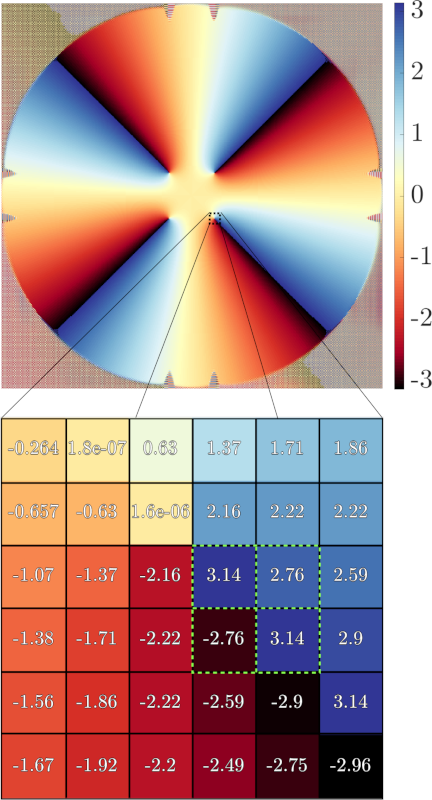
\includegraphics[width = 0.5\textwidth]{data/gpu/vortex_tracking/phi_grid.png}
\caption{An example phase plot of a condensate with four vortices.
The inset shows the values of the grid around each vortex location and highlights where the sum is $2\pi$ for vortex tracking.
}
\label{fig:phase}
\end{figure}

Instead, the phase can be used to uniquely identify vortex locations, as shown in Figure~\ref{fig:phase}.
In the highlighted region, all elements sum to a value of $2\pi$.
In this way, vortex tracking essentially transforms into the task of locating all the $2\pi$ phase windings in the simulated domain via minimization routines where we attempt to find any four grid elements whose sum is $2\pi$.
This process also necessitates a mask for regions outside of the BEC domain, as these regions create spurious $2\pi$ phase windings because of the density is roughly zero outside of the condensate region. 
Further discussion on how to refine this position can be found in previous work~\cite{o2017, docs}.

In three dimensions, vortices are no longer confined to a plane and can extend in any direction, so long as the vortex lines either end at the end of the superfluid or reconnect in the form of vortex rings or more complicated vortex structures.
Tracking three-dimensional vortices is a much more difficult problem which does not have many solutions in superfluid simulations where the superfluid does not fill the simulation domain.
The current state-of-the-art solution has been proposed by Villois \textit{et al}~\cite{villois2016}, and requires finding density dips in the superfluid as initial guesses as to where a vortices might exist.
From there, a vorticity plane is determined and the entire vortex is discovered by moving perpendicularly to the vorticity plane at each gridpoint.
This is a tedious and time-consuming process that does not lend itself well to GPGPU computation without communication between the host and device.
Because some systems simulated with GPUE do not fill the contents of our simulation domain, the proposed method will not work without some modification.
We could still use the method if we have some understanding of the trapping geometry to mask out regions beyond the condensate density; however, as we discussed in Chapter~\ref{ch:splitop}, this is not always the case with gauge fields.
As such, we are currently seeking a more computationally efficient method for tracking vortices in three dimensions, and some thoughts on how this could be done can be found in the Conclusion~\ref{ch:conclusion}.

\begin{figure}
\center 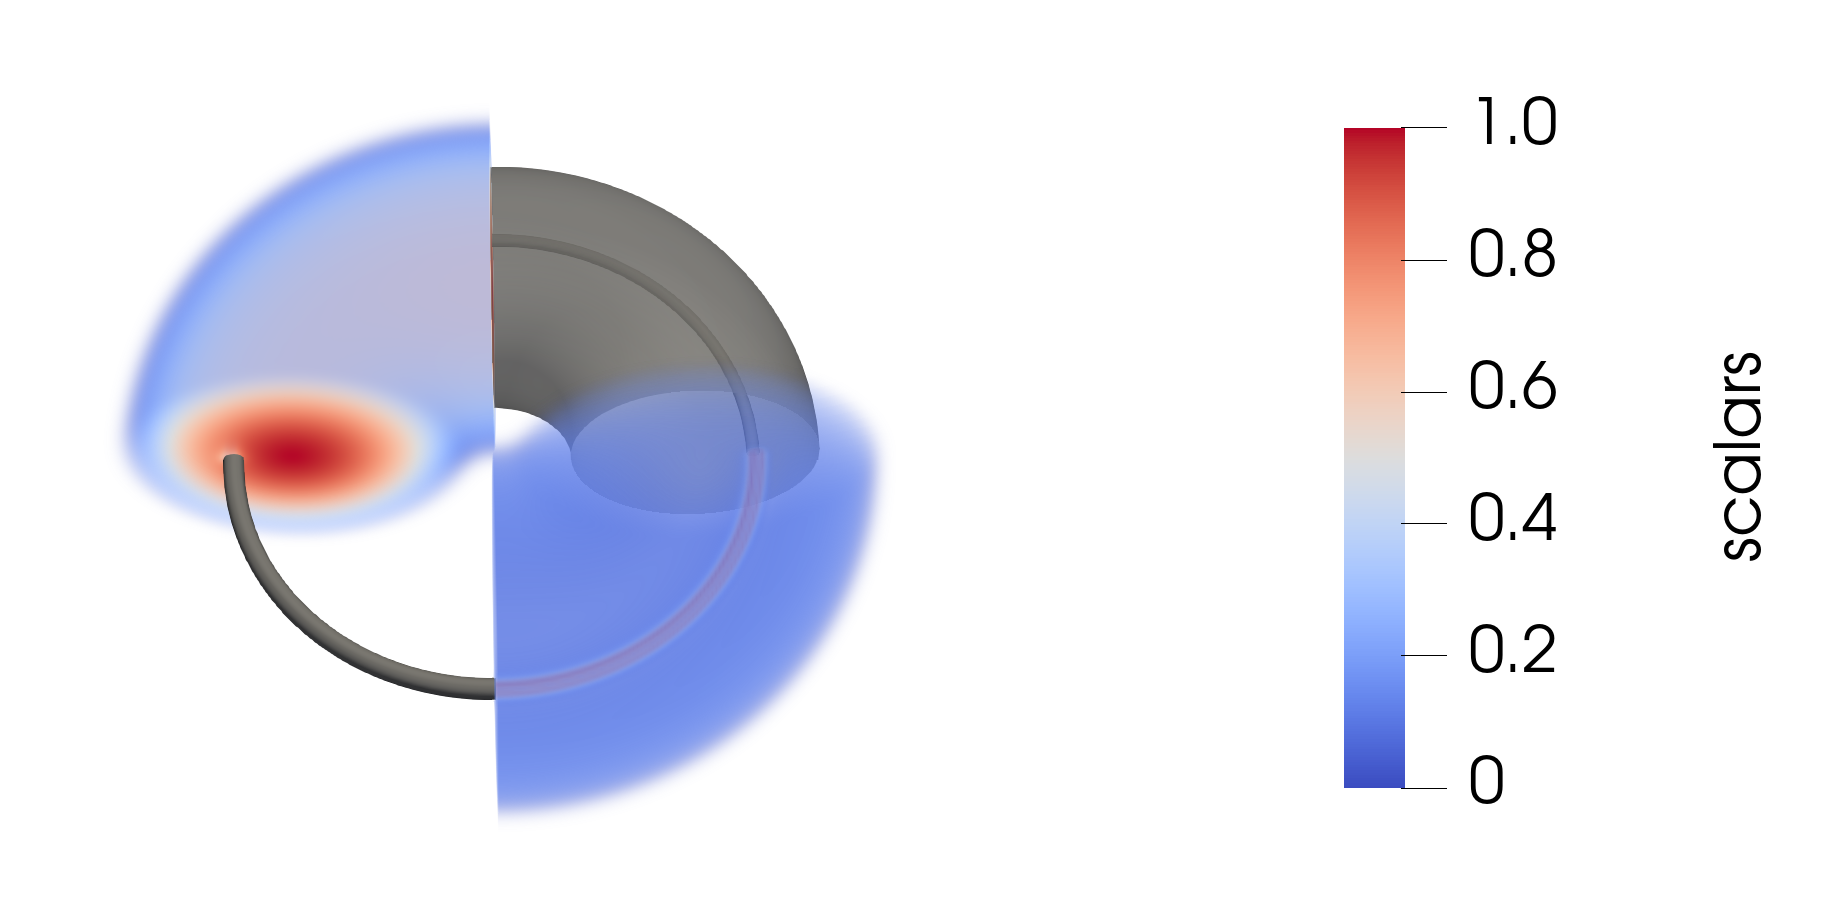
\includegraphics[width=0.75\textwidth]{data/gpu/vortex_highlighting/all.png}
\caption{
An example of vortex highlighting with a Sobel filter.
The upper left quadrant is the superfluid density with no modifications and the upper right quadrant is an isosurface of the density with an opacity of 0.6.
Note here that if there is no opacity set, it is not possible to see the vortex because it is obscured by the outside boundary of the BEC.
The lower right quadrant is the superfluid density after Sobel filtering and the bottom left quadrant is an isosuface on the Sobel filtered density.
Here, we can easily create isosurfaces of vortices that would be occluded when using the density, alone.
The scale varies depending on whether it is coloring the normalized wavefunction density or the filtered density.
}
\label{fig:highlight}
\end{figure}

For these reasons, instead of focusing on vortex \textit{tracking}, I have instead implemented a simple vortex \textit{highlighting} scheme for three dimensions.
This can be done with a Sobel filter on the condensate density, and can easily create crisp visualizations like those found in the computer graphics literature~\cite{guo2018}.
An example of a vortex highlighted wavefunction density, along with an isosurface of both the density and the highlighted density can be seen in Figure~\ref{fig:highlight}.
In this figure, we show that the density after being Sobel filtered can be more easily used to isolate vortex structures without the background BEC.
Though it would be possible to use further edge detection methods, such as the Canny edge detector~\cite{canny1986}, this would add a significant computational overhead and thus was not implemented in the current work.
The problem of efficiently tracking vortex skeletons in three-dimensions is a difficult problem that requires further study; however, vortex highlighting is enough for most three dimensional vortex simulations.
In Chapter~\ref{ch:vortex_states}, we show and example simulation where vortex highlighting has been used to determine the vortex isosurfaces.

\subsection{Energy calculation for superfluid simulations}

As discussed in Chapter~\ref{ch:splitop}, energy calculations can play an essential role in SSFM simulations and can be used to help understand vortex dynamics in certain simulations.
More importantly, energy calculations lie at the heart of convergence criteria for imaginary time propagation.
Essentially, in order to avoid unnecessary computation, many SSFM implementations will cease simulating the system in imaginary time when the change in energy every timestep drops below a certain threshold value.
Though this option is available in GPUE, it is not a native feature for at least three important reasons:

\begin{enumerate}
\item Certain systems, such as large vortex lattices with high rotation, have a seemingly degenerate ground state with different vortex configurations~\cite{o2017, o2016, o2016topo}.
\item GPUE is often run on a computing cluster where the maximum simulation time is set before-hand.
For this, the user must be able to estimate the duration of their simulation, and this is not straightforward if imaginary-time propagation finishes at an unknown time.
\item The energy calculation is memory and operation-intensive and requires at least one additional object of the size of the wavefunction to be created and stored on GPU memory.
\end{enumerate}

\noindent The first and second of these are somewhat self-explanatory, but the third requires further elucidation.

Energy calculations in GPUE are essentially composed of the following operation,

\begin{equation}
E = \braket{\Psi|\mathcal{\hat H}|\Psi}
\end{equation}

\noindent The first problem with this operation is that it requires a summation for the final energy value, and as discussed, this is a poorly-suited problem for GPU hardware.
Even though a robust implementation of parallel reduction has been implemented in GPUE, this is still a slow process.
The next problem comes from the nature of the Hamiltonian, itself.
As described in Chapter~\ref{ch:splitop}, the Hamiltonian is essentially composed of three separate components for vortex simulations:

\begin{align}
\mathcal{\hat H}_v &= V_0 + g|\Psi|^2 + \frac{m\mathbf{A}^2}{2} \\
\mathcal{\hat H}_p &= \frac{p^2}{2m} \\
\mathcal{\hat H}_{pv} &= p\mathbf{A}
\end{align}

\noindent where $\mathcal{\hat H}_v$, $\mathcal{\hat H}_p$, and $\mathcal{\hat H}_{pv}$ are the Hamiltonians in position-space, momentum-space, and mixed-space, respectively.
These operations can be considered with expression trees; however, for three-dimensional simulations they still require either a set of forward and inverse FFT's or a derivative function with fixed stride along with the parallel reduction operation.
This ultimately amounts to the same number of operations required for a single step of imaginary-time evolution; however, because the simulated wavefunction cannot be influenced by the energy calculation, the operation requires at least one additional allocation of a wavefunction-sized array.
Due to the computational time required for each energy calculation, users are requested to input the set of timesteps they would like to compute the energy for before-hand.
In addition, at certain points, it is impossible to run GPUE with the energy calculation, simply because there is not enough memory available on the device.

Though finding the energy of the wavefunction is a useful feature for certain simulations, it should not be used regularly for memory-limited tasks or tasks that should be performed quickly.
Even so, for most applications of GPUE on HPC environments, there should be no problem running the energy-calculation alongside the simulation, itself.

\subsection{Similar software packages}
\jrs{Discuss other software here, like XMDS}

\subsection{Future direction and multi-GPU development}
\label{sec:multiGPU}

At this point, I would consider GPUE to be close to feature-complete.
It is capable of simulating a wide-variety of quantum systems and can even perform dynamic quantum engineering studies with minimal fileIO.
Though more work can be done to maximize instruction throughput, this will not significantly improve the performance of the code because it relies heavily on double-precision.

The next logical step for GPUE development is scaling to larger simulations.
This means that we either need to increase the number of GPUs used for the simulation or decrease the size of the wavefunction, itself.
Though the CSSFM method~\cite{bayindir2015} should allow for the latter, it was ultimately found unsuitable for general-purpose simulations.
As such, the next logical progression is to scale GPUE to multiple GPU devices; however, as I hope to have impressed by now, this is not a trivial task.
Even though the CuFFT library can support multiple GPU devices, this comes with a huge performance penalty, especially for the \texttt{cufftPlanMany(...)} functionality.
To scale to multiple GPU devices efficiently, while still using the SSFM, a large-scale, in-place, multi-GPU transpose is required to ensure proper memory coalescence for FFT routines, which eliminated the need for \texttt{cufftPlanMany(...)} in GPUE.

For this reason, development of GPUE.jl has begun, which has similar performance to GPUE, but is currently lacking the expression tree functionality.
Once GPUE.jl is at feature parity with GPUE, it will become the primary software package for future development.
Ultimately, the Julia language allows for the development of GPUE in a much more maintainable fashion, and also allows for the accessing of GPU hardware in a more convenient way.
In addition to this, Julia allows for more modular development of certain features, such as the DistributedTranspose.jl package that should allow for multi-GPU transposes when fully developed.

\section{DistributedTranspose.jl}
\label{sec:DT}

At its heart, the two-dimensional transpose is a straightforward operation consisting of a swapping of all row and column elements.
Unsurprisingly, this is a difficult task to ensure memory coalescence, but
it is possible to perform a two-dimensional transpose at the same performance as a simple copy, so long as the operation is out-of-place in memory, the operation is performed on shared memory tiles, and bank conflicts are avoided by padding the data structure being transposed~\cite{harris2013}
The transpose becomes even more difficult to create when we wish to transpose large three-dimensional matrices, potentially spanning across multiple GPU devices, while also ensuring the operation is in-place in memory.

In principle, there are three types of three-dimensional transposes:

\begin{description}
\item[Simple Copy]{A benchmark for other transpositions,
    \begin{align}
    A_{xyz} &\rightarrow A_{xyz}
    \end{align}}
\item[Involution]{A transpose where a two-dimensional transpose is operated on a three-dimensional data structure,
    \begin{align}
    A_{x\mathbf{yz}} &\rightarrow A_{x\mathbf{zy}} \\
    A_{\mathbf{xy}z} &\rightarrow A_{\mathbf{xy}z} \\
    A_{\mathbf{x}y\mathbf{z}} &\rightarrow A_{\mathbf{z}y\mathbf{x}}
    \end{align}}
\item[Rotation]{A fully three-dimensional transpose,
    \begin{align}
    A_{\mathbf{xyz}} &\rightarrow A_{\mathbf{yzx}} \\
    A_{\mathbf{xyz}} &\rightarrow A_{\mathbf{zxy}}
    \end{align}}
\end{description}

It has been shown that for out-of-place transpositions, it is possible to perform all of these operations as efficiently as a a simple copy; however, in-place rotational transposes can only attain 60-70\% of the performance based on currently known methods~\cite{jodra2015, el2008}.
In addition, distributed transposes of this nature have not been discussed except for on an out-of-place array~\cite{ruetsch2013}.

At its current state, the DistributedTranspose.jl package is able to do out-of-place, distributed transposes; however, when feature-complete, it should allow for the implementation of new distributed methods for such computation.
It should be mentioned that this package has potential to be used by many other software packages that require using spectral methods on multiple GPU devices.
Often, HPC engineers prefer finite-element or difference methods when computing large-scale fluid flow because these methods scale much better across distributed systems; however, with an appropriate distributed transpose methods, it might be more optimal to perform spectral simulations in certain regimes over other methods.

\section{Outlook}

In this chapter, I presented the fundamentals of GPGPU, along with the GPUE codebase for simulating superfluid vortex systems.
It is important to note that GPU architecture is best at embarrassingly parallel tasks, and as such, the SSFM is severely limited by its FFT routines; however, because one-dimensional FFT operations on GPU devices are often faster for larger matrix sizes than their CPU-based counter-parts~\cite{merz2016}, it seems that the SSFM is better suited for GPU architecture.
In this chapter, I also discussed important optimizations done in GPUE to ensure proper utilization of GPU architecture for dynamic simulations of dynamic superfluid vortex simulations in two and three dimensions, including expression trees, FFT optimizations, vortex tracking and highlighting, methods used to decrease GPUE's storage footprint, and GPUE.jl.
Finally, I discussed the future development of the DistributedTranspose.jl package, which should allow for large-scale spectral methods to be suitable for distributed GPU systems, often found in HPC environments.

For Chapters~\ref{ch:2d} and \ref{ch:vortex_states}, I will discuss two physical examples that were enabled by the GPUE codebase, also highlighting future physical directions and re-enforcing the future directions discussed here.

\chapter{Vortex analysis of two-dimensional superfluid systems}
\label{ch:2d}

Here, we show an application of the GPUE codebase in simulating a two-dimensional chaotic system with few vortices.
This chapter makes heavy use of the vortex tracking, rotation, and phase-imprinting methods described in Chapter~\ref{ch:gpu}.
In addition, this chapter intends to display the dependence of post-processing metrics to dynamical studies of superfluid systems.

In a similar fashion to Chapter~\ref{ch:1d}, this chapter will start with a disclaimer about the dimensionality of the systems we will be simulating.
In principle, all real-world physics is three-dimensional, but in a similar fashion to how a one dimensional cigar-shaped BEC can be created, a pancake-like geometry can also be constructed by increasing the trapping frequency in the $\hat z$ (perpendicular) direction with respect to the $\hat x$ and $\hat y$ (transverse) directions.
With this geometry, we can assume that the condensate is in the ground state along the $\hat z$ dimension and rewrite the wavefunction as $\Psi(\mathbf{r},t) = \Psi(x, y, t)\phi(z)$, where $\Psi(x, y, t)$ is the wavefunction in the transverse plane and $\phi(z) = (m \omega_z/(\pi\hbar))\text{exp}(z^2 m\omega_z/(2\hbar))$ is the ground state along the $\hat z$ dimension.
By integrating over $\hat z$, we also find that the interaction strength is modified for a two-dimensional consensate to be

\begin{equation}
g_{2D} = g \sqrt{\frac{m\omega_z}{2\pi\hbar}}.
\end{equation}

\noindent With these changes, we can simulate two-dimensional quantum simulations with the GPUE codebase~\cite{zhang2019, o2017, o2016topo, o2016}.

This chapter will apply several of the techniques mentioned in Chapters~\ref{ch:splitop} and \ref{ch:gpu} to a rotating two-dimensional BEC system for a small number of vortices and will follow the work of Zhang \textit{et.al.}~\cite{zhang2019}.

\section{Chaotic few-body vortex dynamics in rotating Bose--Einstein condensates}

Chaotic evolution is typically identified by a significant divergence in trajectory based on a small change in the initial conditions~\cite{strogatz2018}, and it is possible to find such an environment in turbulent flows~\cite{spiegel1987, biferale2005}.
For classically turbulent flow, the degree of chaos depends on the Reynolds number~\cite{berera2018}; however, the nature of quantum turbulent effects is still an active area of research~\cite{white2014}.
Because superfluid vortices are relatively simple compared to their classical counterparts, there has also been significant interest in the differences between classical and quantum turbulence~\cite{nemirovskii1995,kyriakopoulos2014,koukouloyannis2014,navarro2013}.
In spite of the differences between the fluid models, vortex dynamics in superfluid systems are remarkably similar to classical point-vortex models and key features of classical turbulence, such as the Kolmogorov spectrum have been shown to exist for large, turbulent, quantum systems~\cite{nore1997,stalp1999,araki2002,salort2010}.

In this study, we would like to create a quantum system that is chaotic without relying on quantum turbulence, and
it is known that it is not possible to excite quantum chaos in large vortex lattices, as these systems have been proven to be stable to external perturbations~\cite{o2017}.
For this reason, we wish to probe quantum chaos with a small number of vortices, such that quantum tuburlent effects are not excited.
These chaotic, few-vortex systems have been studied previously by Aref and Pomphrey~\cite{aref1982, aref1980, aref1983}, who showed that quantum chaos can be excited in systems with as few as four vortices in an infinite plane~\cite{aref1982}.
Unlike classical chaos, the onset of quantum chaos seems to appear with fewer vortices present, and few-vortex systems have been explored experimentally for two, three, and four vortices in harmonically trapped BECs~\cite{navarro2013}.
When analyzed with a reduced Hamiltonian approach, harmonically trapped BECs seem exhibit chaotic effects with as few as three vortices, two co-rotating vortices and an anti-vortex rotating in the other direction~\cite{kyriakopoulos2014,koukouloyannis2014}.

Experimentally, it is now possible to detect vortex circulation~\cite{seo2017}, image vortices in-situ~\cite{wilson2015}, and probe vortex dynamics at different times within a single experiment~\cite{freilich2010, serafini2017}.
Because quantum vortices are simple and BECs are highly controllable experimental systems in two-dimensions, there has been significant interest in two-dimensional quantum turbulent systems as well~\cite{neely2013,shin2004}.
Additional effects, such as the K\'arm\'an vortex street~\cite{kwon2014} and Onsager vortex clusters~\cite{gauthier2018,johnstone2018} have also been shown to exist experimentally.

In order to engineer well-controlled initial conditions, we will create a small vortex lattice of four vortices, and then create a small defect via phase imprinting.
This process will controllably induce chaotic vortex dynamics in an experimentally feasible way.
We also show that these chaotic dynamics are enhanced by the close approach of vortices in the simulated results.
By using phase imprinting in this way on a larger number of vortices in a vortex lattice, it might be possible to induce chaotic events there as well, which might enable studying a set of vortex trajectories that is chaotic at specific points, but stable overall.

\section{Model}

\begin{figure}
\center 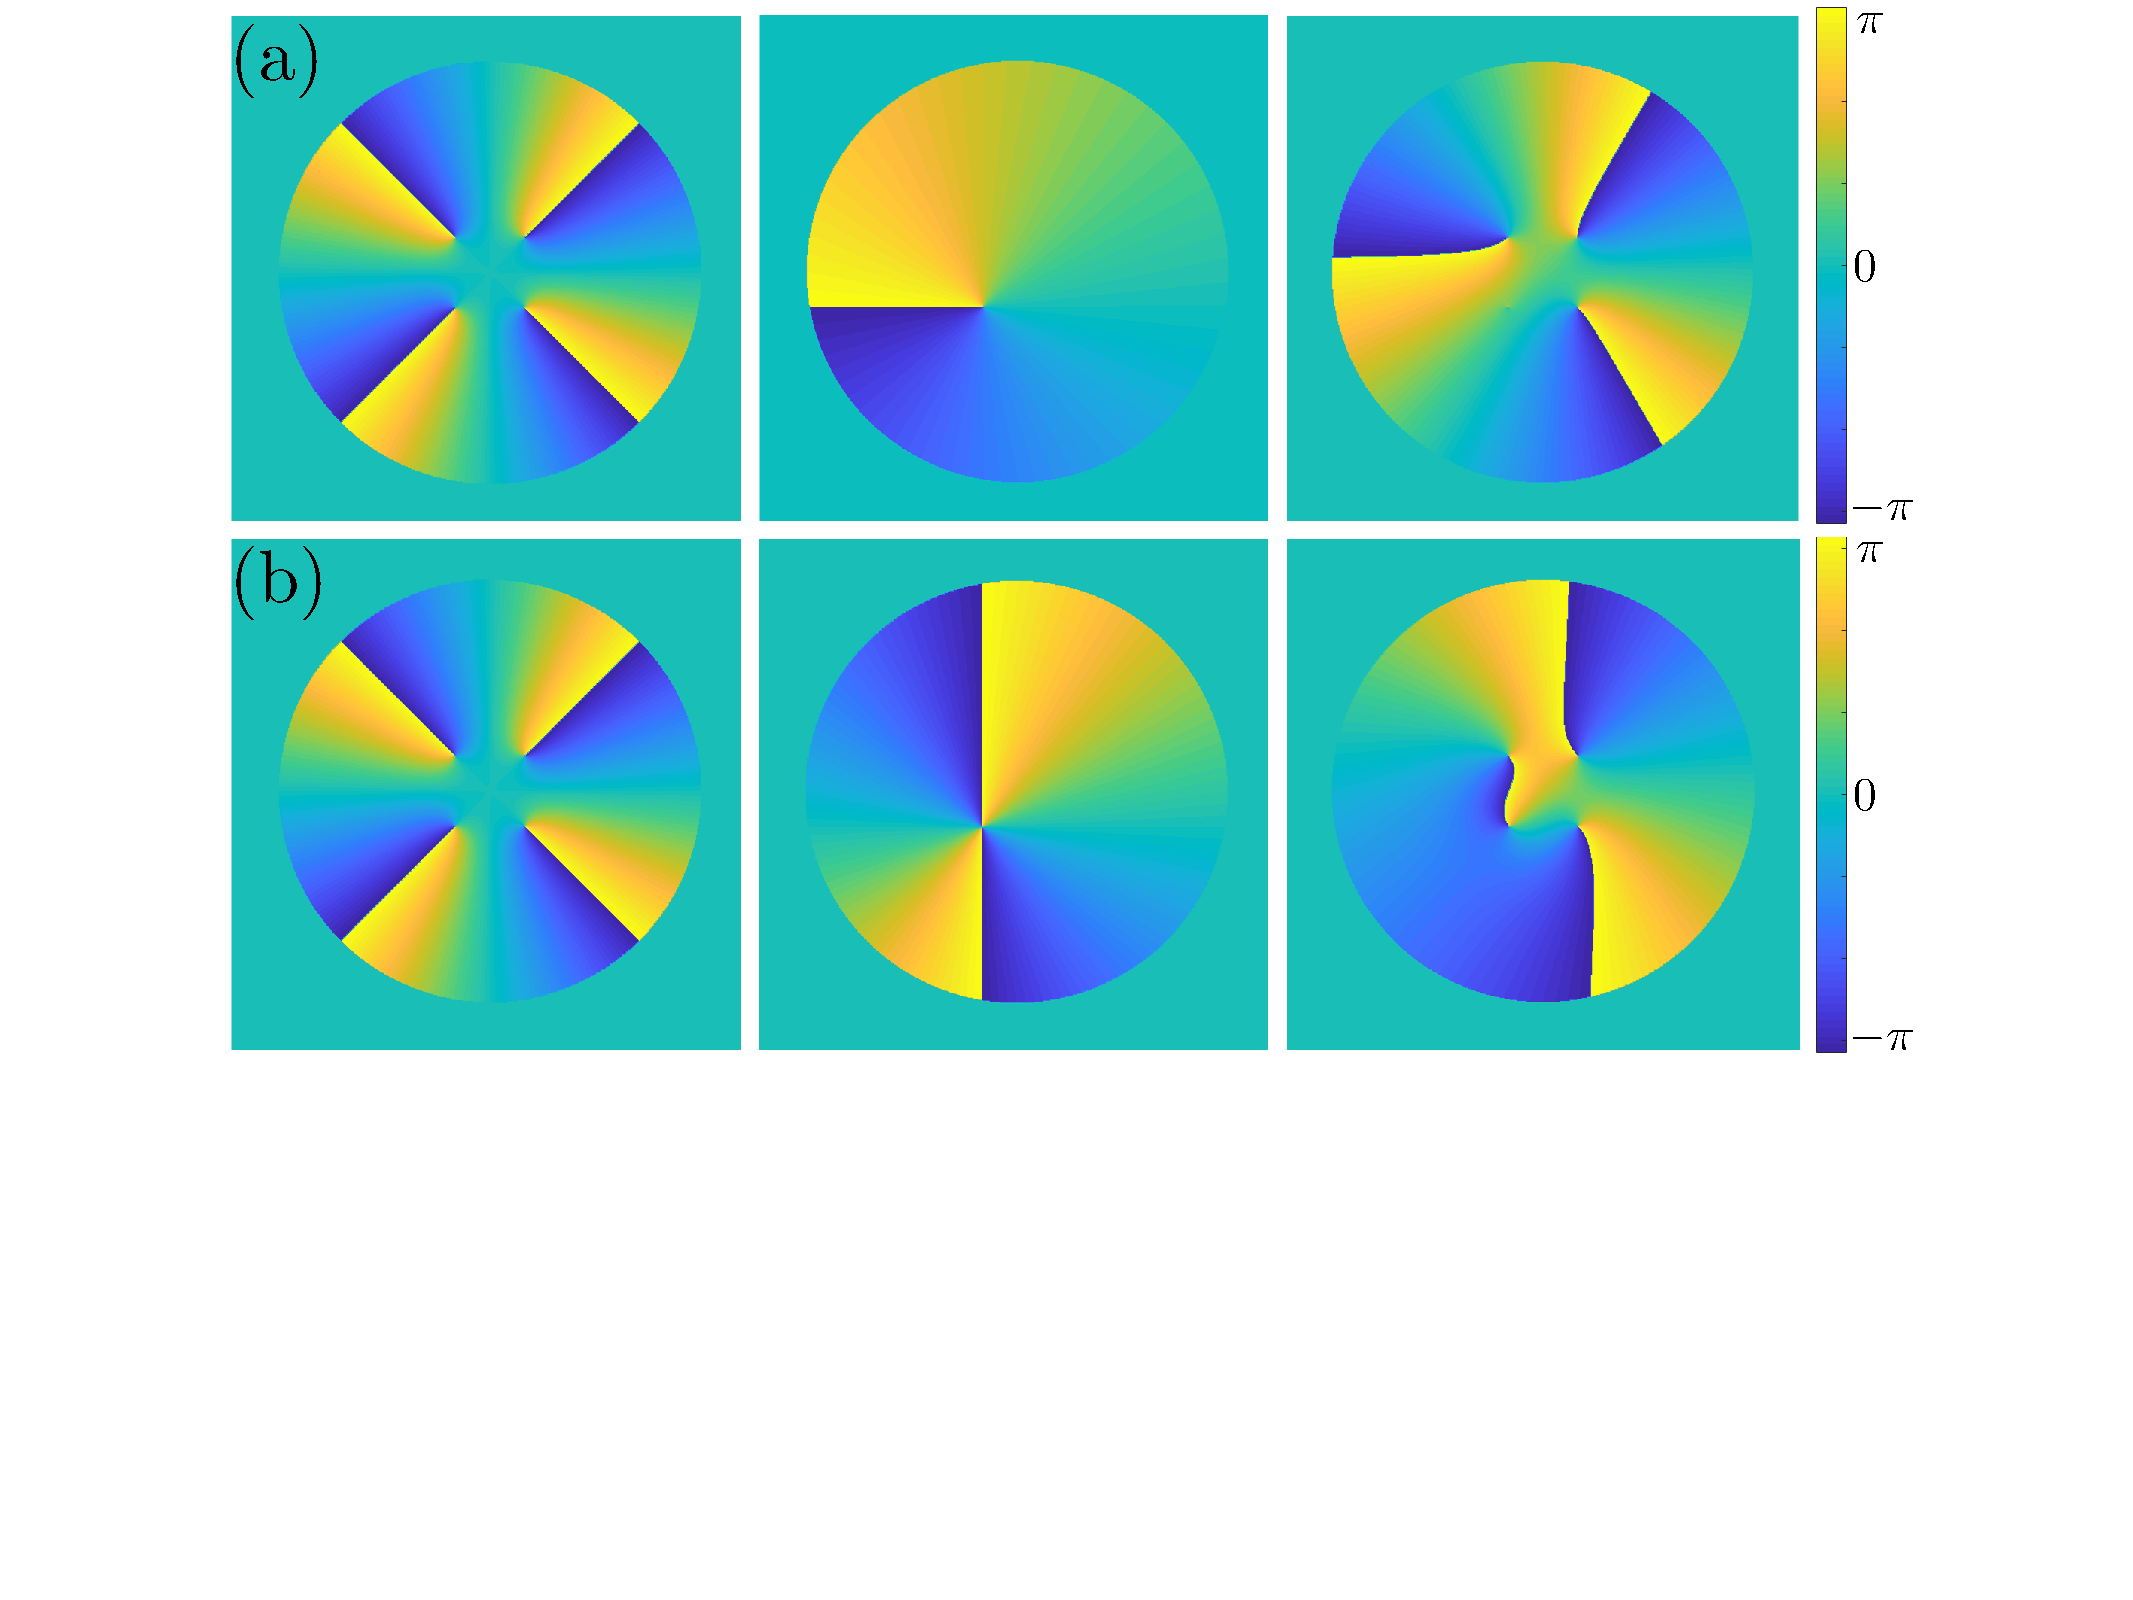
\includegraphics[width=0.75\textwidth]{data/2d/phase/phase}

\caption{
The initial four co-rotating vortex system is shown at the left.
In the center is the applied phase mask of $-2\pi$ for (a) and $-4\pi$ for (b), and the resulting phase distribution is shown on the right.
Here we see that by applying a $-2\pi$ phase winding, we erase a vortex from the system, and by applying a $-4\pi$ phase winding, we flip the vortex, creating an anti-vortex.
}
\label{fig:phase}
\end{figure}


For this study, we created a condensate with $N = 10^6$ $^{87}$Rb atoms with an s-wave scattering length of $a_s \approx 90a_0$ in a pancake geometry with typical trapping frequencies of $(\omega_\perp, \omega_z) = (2\pi, 32\pi)$Hz.
Here, the s-wave scattering length is $a_s \approx 90a_0$ and the effective interaction strength is $g = 6.8\times 10^{-40}$ m$^4$kg/s$^2$.
These simulations were performed on a grid of $2^{10} \times 2^{1-}$ points and covering an extent of $700\mu \text{m} \times 700 \mu \text{m}$

First, ground-state evolution was performed with a low rotation frequency of $\Omega = 0.3 \times 2\pi$ Hz via GPUE~\cite{schloss2018}.
Though large rotational frequencies will create a triangular lattice, for smaller frequencies, other configurations are known ~\cite{aftalion2001}, and we will focus on the regine where the ground state is composed of four vortices in a square configuration~\cite{zampetaki2013}.
Once this configuration is achieved, we then manipulate a vortex via phase imprinting, such that three co-rotating vortices and one anti-vortex exist in the system.
Examples of phase imprinting on this system can be seen in figure~\ref{fig:phase}, where the top row shows a simple vortex annihilation and the bottom row shows a vortex flip.

\section{Regular and irregular vortex dynamics}

\begin{figure}
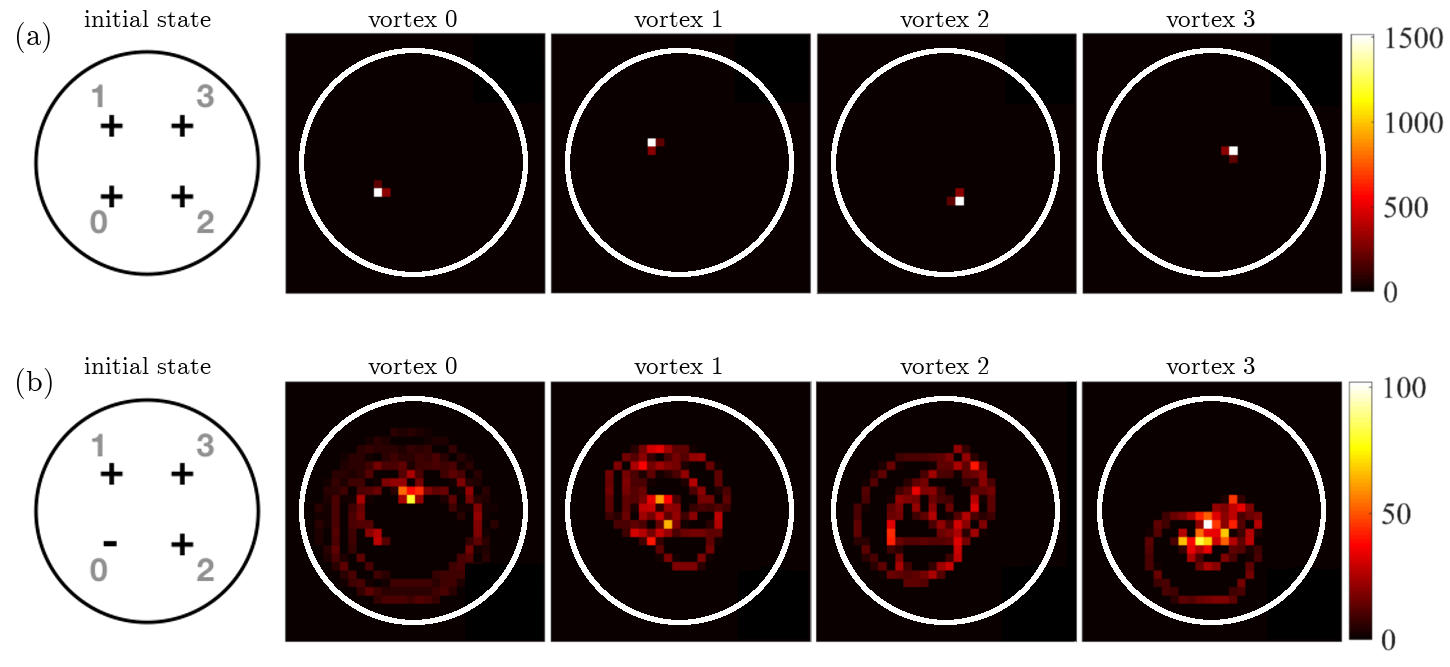
\includegraphics[width=\textwidth]{data/2d/histogram/histogram}

\caption{
Histograms of the positions of each vortex in the transversal plane for 20 secons in the co-rotating frame.
The lower left vortex has been annihilated and re-imprinted with (a) the same and (b) the opposite direction of rotation, exactly on the location of the previous vortex.
The area of each plot is $400\mu \text(m) \times 400 \mu \text{m}$, and the white circles correspond to iso-lines at 40\% the maximum density to highlight the extent of the vortex motion.
In (a), we see that if all four vortices are co-rotating, regular trajectories appear, but in (b), we see that flipping the rotation direction of a single vortex creates disordered trajectories.
}
\label{fig:histogram}
\end{figure}

It is known that a lattice of vortices with the same direction of rotation will exhibit regular dymanics~\cite{abo2001}, and in Figure~\ref{fig:histogram}(a), we confirm this for a system of four vortices.
In this figure, we show a histogram of the vortex trajectory over 20 seconds of evolution when removing and then re-imprinting a vortex of the same rotational direction at the same location
Even though a small residual movement appears due to small phonon excitations that were not fully removed from the imaginary time evolution, the vortices remain stationary.
In Figure~\ref{fig:histogram}(b), we also show that if the re-imprinted rotation is of the opposite direction, the vortex dynamics become more disordered, with vortices traversing a larger width of the condensate.
It is worth mentioning that these histograms can be constructed experimentally with available imaging techniques~\cite{wilson2015,freilich2010}.

\begin{figure}
\center 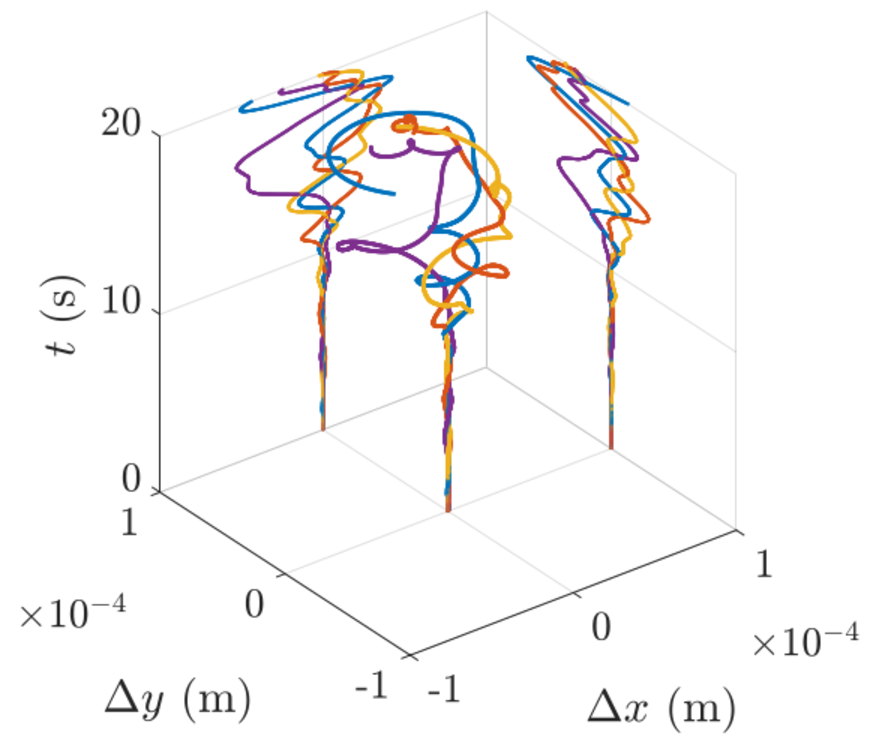
\includegraphics[width=0.5\textwidth]{data/2d/evolution/evolution}

\caption{
Evolution of the difference in trajectories $\triangle \textbf{r}_i = \textbf{r}_{i}-\textbf{r}'_{i}$ with $\textbf{r}$ corresponding to the position of the $i$th vortex from the center of the condensate and $i\in \{0,\ 1,\ 2,\ 3\}$ labelling each individual vortex for the four-vortex system as shown in Fig.~\ref{fig:histogram}.
A small change in the initial position of the anti-vortex arises from a phase-imprint at $(x_{0},y_{0})$ and $(x_{0}-\xi/3,y_{0})$ where $(x_{0},y_{0})$ denotes the pre-existing co-rotating vortex core position.
The curves show that even though the onset of disorder is immediate, a strong divergence of trajectories is observed at about $t\approx 10 \text{s}$ (see projections onto the $x$-$t$ and $y$-$t$ planes).
The difference in trajectory of the anti-vortex, $\Delta \mathbf{r}_0$, is shown in blue, while yellow, orange, and purple lines depict the three co-rotating vortices.
}
\label{fig:evolution}
\end{figure}

Even though the introduction of the anti-vortex creates a disordered trajectory, it could be entirely possible that this trajectory is stable.
To uniquely identify chaotic behaviour, we need to show that any small perterbation in the vortex location will also provide a significantly different trajectory.
To check this, we compare two sets of vortex trajectories with slightly different shifts in the initial position of the anti-vortex, $\mathbf{r}_0$ and $\mathbf{r}'_0$, where $\mathbf{r}_0 - \mathbf{r}'_0 = \xi/3$ and $\xi$ is the healing length.
In Figure~\ref{fig:evolution}, we show the differences in trajectories, defined as $\Delta \mathbf{r}_i(t) = \mathbf{r}_{i}(t)-\mathbf{r}'_{i}(t)$ in Figure.~\ref{fig:histogram}, where $\mathbf{r}$ refers to the position of the $i$th vortex from the center of the condensate and $i\in \{1,2,3\}$ corresponds to the vortex number.
Here, we see that the difference in trajectory is initially small, but diverges significantly at around $t \approx 10$ seconds, which is a strong indication of chaotic behavior.

After closely inspecting the vortex dynamics (shown in the supplementary movie~\ref{movie}), we see that this strong divergence in vortex trajectories seems to be accelerated when all four vortices come in close proximity.
Because the velocity fields of each vortex decays as $1/\mathbf{r}$, where $\mathbf{r}$ is the distance from the core, the vortices experience stronger velocity fields when they are closer; therefore, the point of minimal separation can be seen as a highly nonlinear multi-vortex scattering event that accelerates the divergence shown in Figure~\ref{fig:evolution}.
In Figure~\ref{fig:snapshots} we study this further by showing snapshots of the condensate density before ($t = 6$s), at ($t = 10$s), and after ($t = 15$s) the scattering event are shown in (a) and (b) for the non-shifted and shifted anti-vortex locations.
The differences between position of each vortex and the anti-vortex is also shown (b) for the case where the anti-vortex is shifted by $\xi/3$.
Here, we see that there is a clear minimum at $t \approx 10$s, which is the same time at which the  trajetories begin to diverge in Figure~\ref{fig:evolution}
In order to characterize this divergence in trajectory, we must analyze the vortex dynamics in more detail and calculate the Lyapunov exponent

\begin{figure}
\center 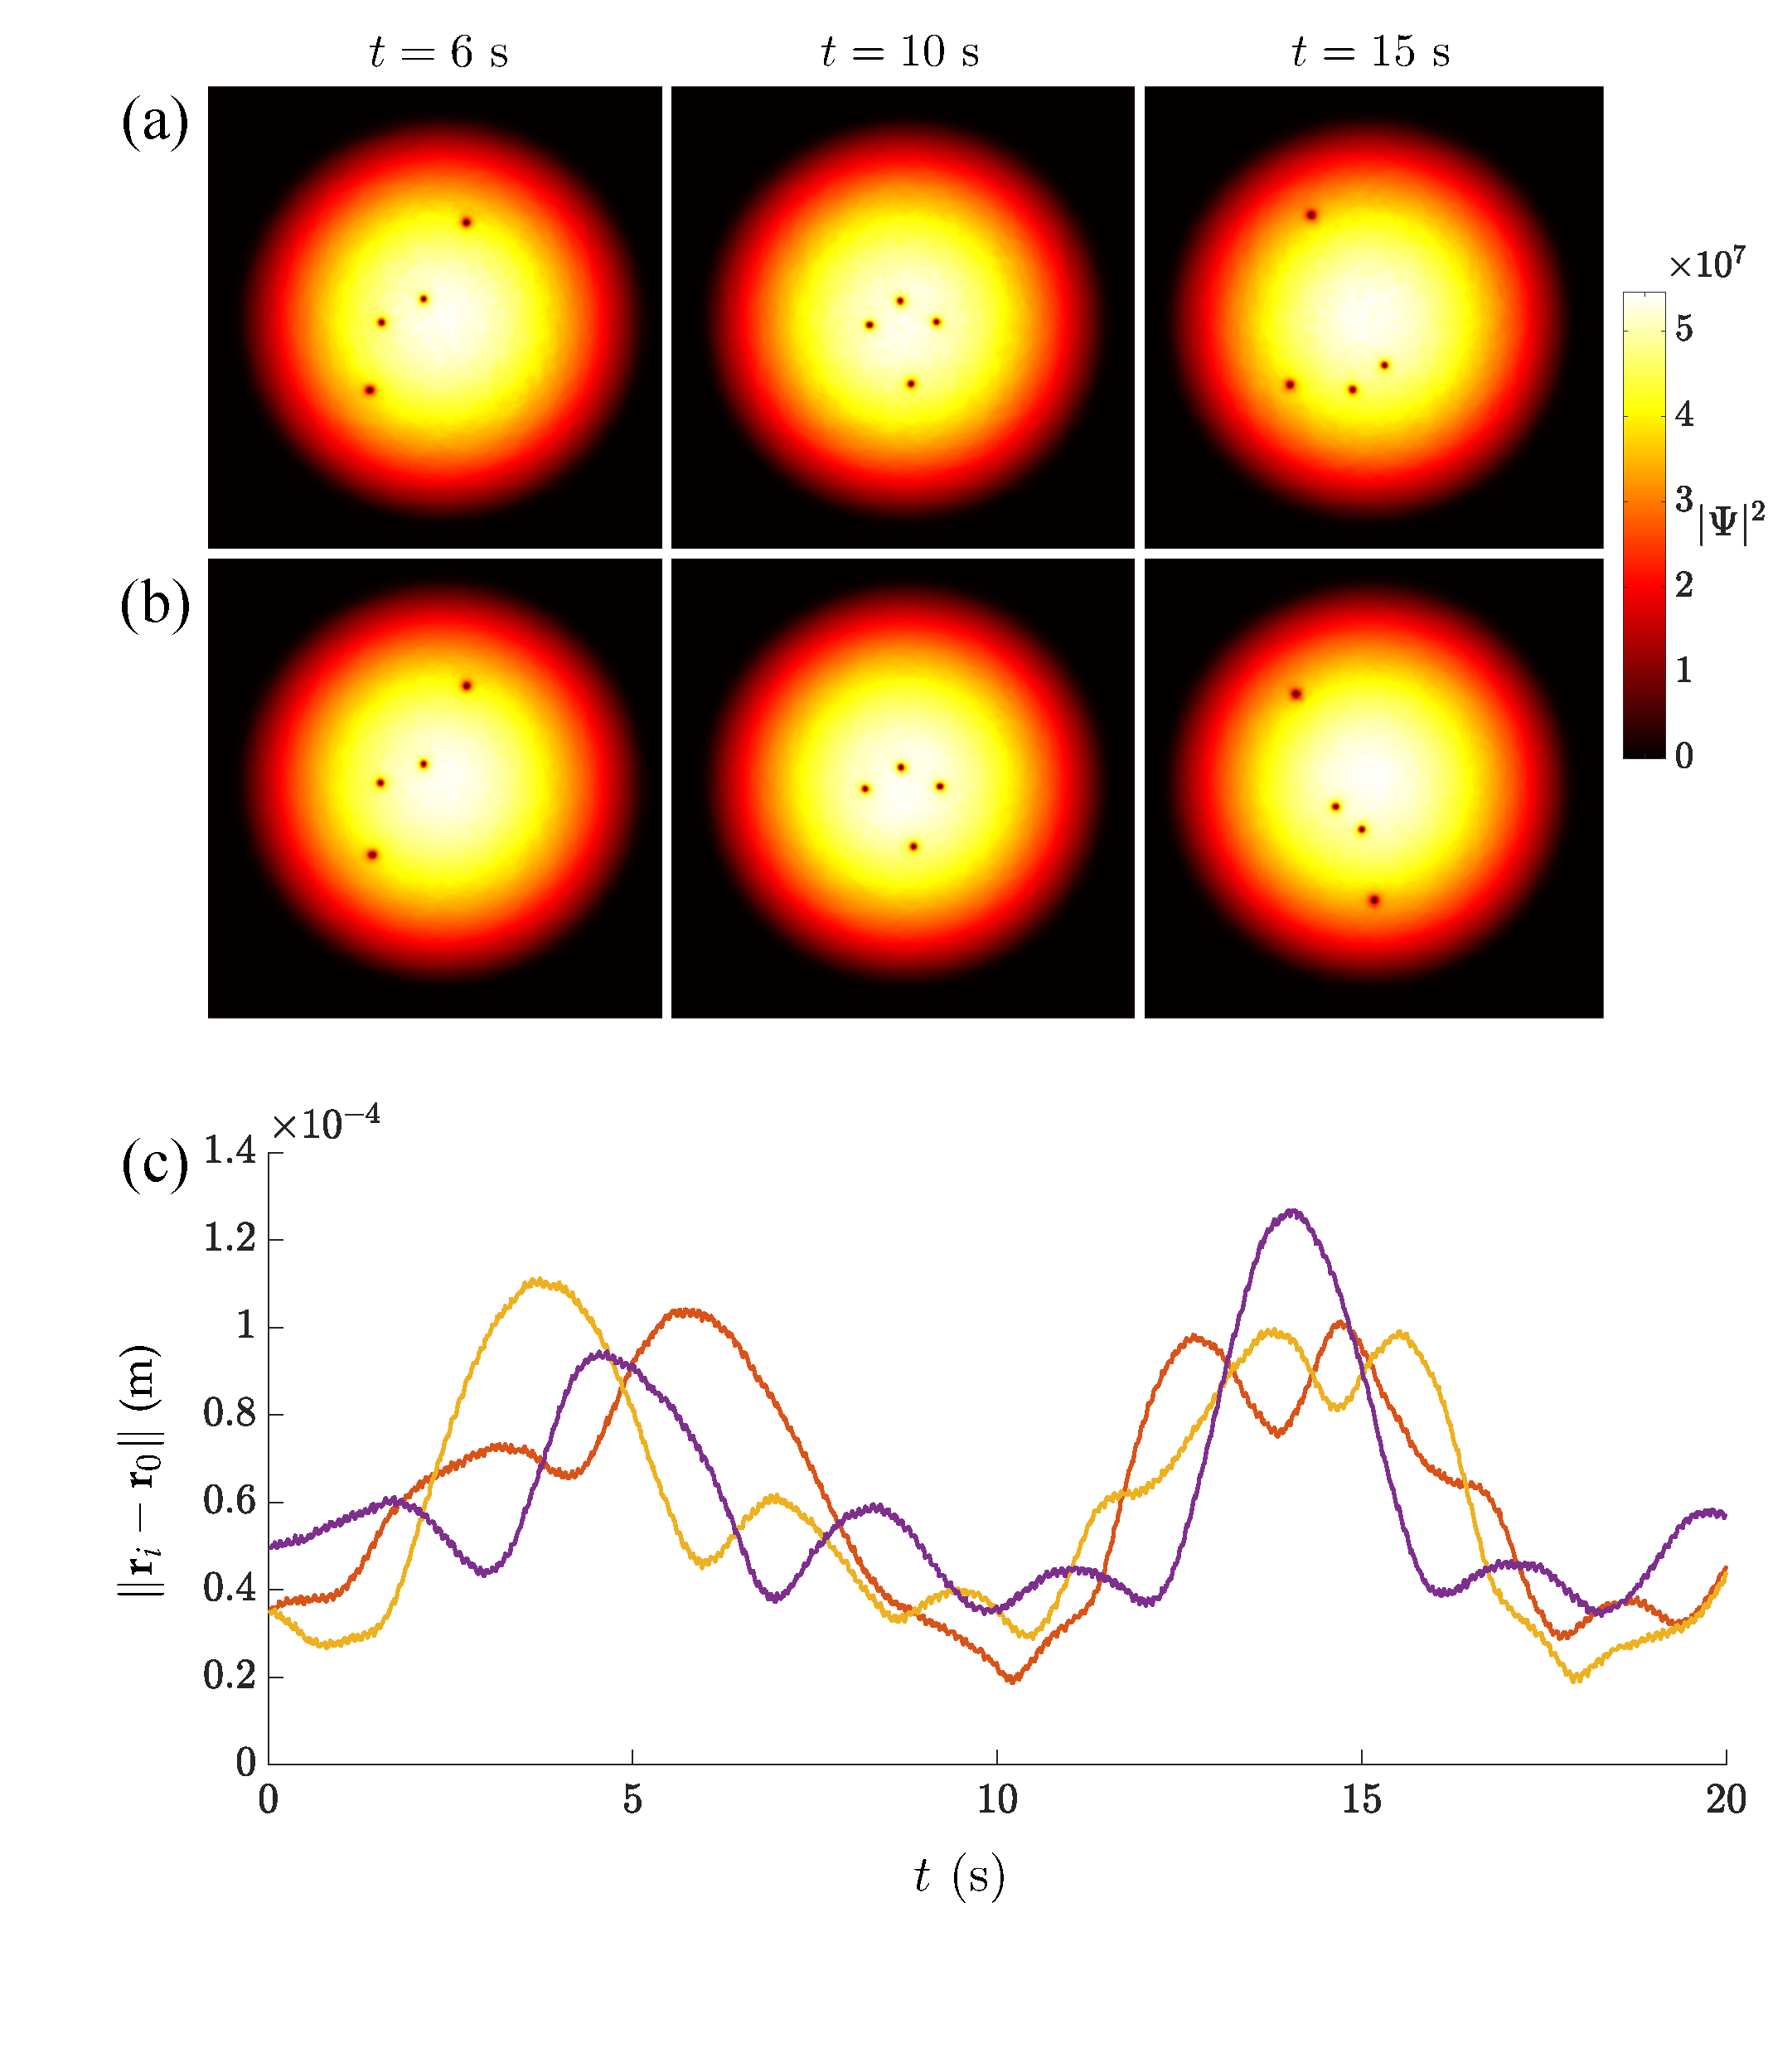
\includegraphics[width=0.75\textwidth]{data/2d/snapshots/snapshots}

\caption{
Density plots of condensate for (a) $\Delta x = 0$ and (b)$\Delta x=\xi/3$ at times $t=\{6,10,15\}$ s. The densities before the scattering event differ only on small scales (see $t=6s$), whereas for times after the event large deviations are visible (see $t=15s$).
At $t=10s$ the vortices make their closest approach. The area plotted is $500 \mu m\times 500 \mu m$.
(c) Distances between the vortices at positions $\mathbf{r}_i$ with $\mathbf{r}$ corresponding to the position of the $i$th vortex from the center of the condensate and $i\in \{1,2,3\}$ corresponding to the vortex number as shown in Fig.~\ref{fig:histogram} and anti-vortex at $\mathbf{r}_0$ for $\Delta x = 0$.
A minimum around $t=10s$ is clearly visible.
}
\label{fig:snapshots}
\end{figure}

\section{Characterizing chaotic vortex dynamics}

\begin{figure}
\center 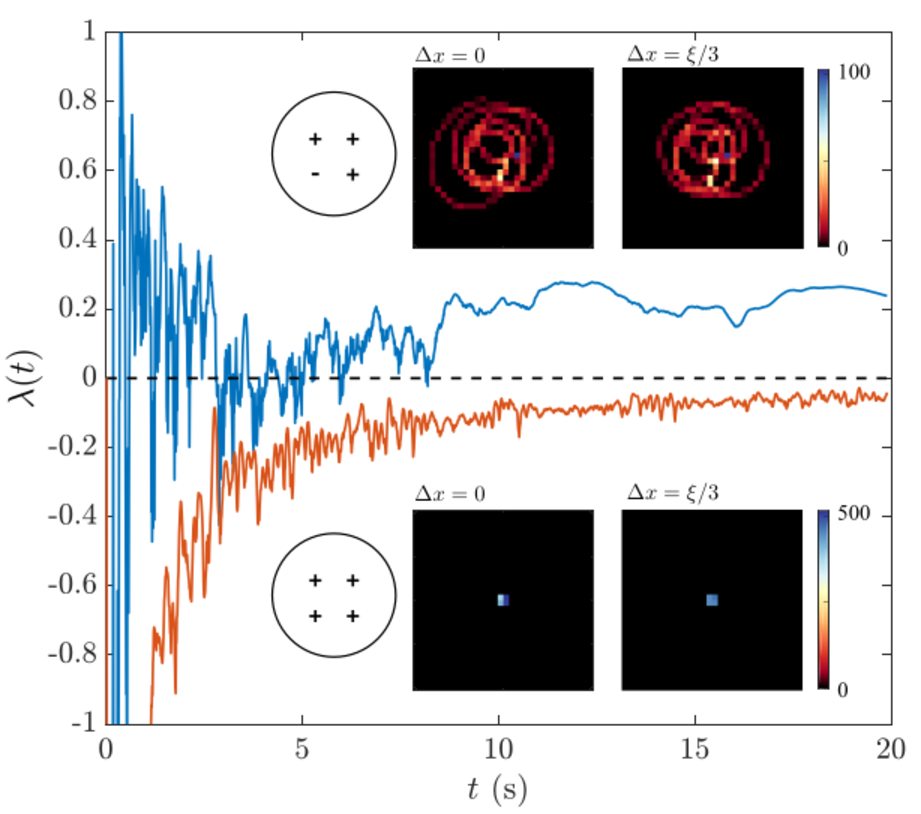
\includegraphics[width=0.75\textwidth]{data/2d/lyap/lyap}

\caption{
The insets show the histograms of the COM trajectories calculated over 20 seconds of evolution for the system of four vortices when the position of a single vortex has been shifted by $\Delta x=0\xi$ and $\Delta x=\xi/3$.
The upper two panels depict the corresponding trajectories after the direction of rotation of a single vortex has been reversed, whereas the lower row displays the trajectories for the case where all vortices co-rotate.
The main curve plots the corresponding Lyapunov exponents,  calculated from the shown COM trajectories. 
The negative Lyapunov exponents (orange) indicate that shifting the vortex about the initial position still ensures the stability of vortex trajectories. Reversing the direction of circulation of a single vortex (blue) however leads to fluctuations about zero, eventually leading to a fully positive exponent. 
}
\label{fig:lyap}
\end{figure}


To characterize the degree of chaos for the shown vortex dynamics, we have chosen to use Lyapunov exponents, which give the rates of divergence for nearby orbits in phase space~\cite{wolf1985}.
With this measure, we track two trajectories in phase space and assume that the divergence between the two trajectories will either exponentially converge or diverge, and we can model this behaviour with

\begin{equation}
|\delta\mathbf{Z}(t)| \approx e^{\lambda t} |\delta \mathbf{Z}_0|.
\end{equation}

\noindent Here, $\delta\mathbf{Z}_0$ is the initial separation between the trajectories and $\lambda$ is a quantity known as the Lyapunov exponent.
If the exponent is negative, it means that the trajectories tend to converge, but it it is positive, the trajectories will diverge, thus indicating chaotic motion.
The rate of divergence is determined by the value of the exponent.

For out simulation, we model the trajectories in four-dimensional phase-space with $\mathbf{P(t)} = (x(t), y(t), v_x(t), v_y(t))$ and $\mathbf{P}'(t) = (x'(t), y'(t), v'_x(t), v'_y(t))$.
The separation is then defined to be $\delta \mathbf{P(t)} = (\delta x(t), \delta y(t), \delta v_x(t), \delta v_y(t))$ where $\delta x(t) = x(t) - x'(t)$, etc.
The exponent can then be calculated as

\begin{equation}
\lambda = \lim_{t\to\infty}\frac{1}{t}\text{ln}\frac{||\delta\textbf{P}(t)||}{||\delta\textbf{P}(0)||}
\label{eqn:lyap}
\end{equation}

\noindent where $||\cdot||$ denotes the Euclidean norm.

In this case, we track each vortex with the methods outlined in Chapter~\ref{ch:gpu}, and use both the position and velocity of the vortex.
Because we wish to determine whether the total system is chaotic, beyond its constituent vortices, we use a center of mass (COM) variable, defined as $\mathbf{R}_M = \frac{1}{n+1}\sum_{i=0}^nr_i$, where $n+1$ is the number of vortices.
Similarly, the center of velocity is defined as $\mathbf{v}_M = \frac{1}{n+1}\sum_{i=0}^nv_i$.
These values are then used with Equation~\ref{eqn:lyap}, and the results are shown in Figure~\ref{fig:lyap}.
The insets in Figure~\ref{fig:lyap} show the histograms of the COM trajectories for the case where an antivortex is and is not present.

As expected, the exponent spectrum calculated in Figure~\ref{fig:lyap} shows that the regular, co-rotating system always shows a negative (converging) exponential value, but the system with the anti-vortex is largely positive (diverging).
During collisional event shown in Figures~\ref{fig:snapshots} and \ref{fig:evolution}, we see that the exponent becomes positive for the duration of the simulation.
It is worth noting that other global measurements could be used instead of the COM, such as the center of charge~\cite{kyriakopoulos2014}, but we found these to provide similar qualitative results to those shown here.


\section{Conclusions}

With this study, we have shown that it is possible to induce chaotic vortex dynamics in few-vortex systems by using phase imprinting to flip the rotational direction of a vortex in two dimensions.
We also show that a scattering event seems to be correlated to a positive Lyapunov exponent and an acceleration of chaotic behaviour.
Though not shown here, we have also performed similar simulations for small lattices of five and six vortices, which seem to still exhibit chaotic dynamics with Lyapunov exponents of 0.24, 0.24, and 0.27 for the four, five, and six vortex cases, respectively after 20 seconds of evolution~\ref{zhang2017}.
This behaviour is radically different than the behaviour of largescale vortex lattices, as similar techniques for these systems have been shown to only cause local disturbances~\ref{o2016topo}.
Further exploration of the crossover from regular to turbulent dynamics, and the crossover from chaotic to stable dynamics for large-scale vortex lattices remains an interesting extension for future work.

This study shows that there is strong utility in simulating two-dimensional quantum gases and highlights dynamic measures, such as the Lyapunov exponent.
Here, it is obvious that fast vortex tracking methods are essential to dyanamical turbulence and chaos modelling, and a major limitation to performing similar studies in three dimensions is the computational hurdle of vortex tracking in this area.
As such, most three-dimensional studies of quantum chaos rely on other methods, such as vortex filament methods which provide vortex skeletons during the simulation, itself.
As mentioned in Chapter~\ref{splitop}, these methods cannot simulate the underlying dynamics of the condensate, and are thus removed from experimental application.
Further extensions of this work in three dimensions would also allow for studies on the movement of the vortex lines, themselves, which were projected onto two-dimensional point-vortices in this model.

For the next study, we will transition into a discussion of three-dimensional vortex dynamics and show an experimentally realistic system to allow for the generation, control, and detection of vortex ring-like systems with artificial magnetic fields.



\chapter{Generation, control and detection of 3D vortex structures in superfluid systems}
\label{ch:vortex_states}

In this chapter, I will discuss another application of the GPUE codebase, this time to the controlled creation of vortex structures in three dimensions with artificial magnetic fields generated by an optical nanofiber.
To the best of my knowledge, this is the first time an experimentally realizable device to generate vortex ring-like structures with a dielectric system has been suggested and investigated, and I also provide a method to detect whether a vortex ring is present in an elliptic-toroidal condensate.
This project encompasses three-dimensional vortices and coupled light-matter systems, so to begin, I will briefly discuss vortices in three-dimensional systems, followed by the model used for this project, where I will describe how the light from an optical nanofiber can generate and control vortex structures in BEC systems.
As a note, even though vortex dynamics are not shown in this study, GPUE is more than capable of simulating these effects, and potential applications of vortex ring dynamics will be discussed in the outlook of this chapter.
The contents of this chapter have recently been submitted to Phys. Rev. Fluids~\ref{schloss2019}.
In this study, I performed all simulations, with exception of vortex states generated in Figures~\ref{fig} and \ref{fig}, which were performed under my supervision by Peter Barnett.
I also designed the GPUE codebase to allow for these simulations and visualized all data.
This project was supervised overall by Thomas Busch and Rashi Sachdeva.


\section{Three-dimensional vortex structures}
\label{sec:vortex}

As mentioned in Chapter~\ref{ch:splitop}, in BEC systems with large amounts of angular momentum and a single axis of rotation, the vortices will create a triangular, Abrikosov lattice~\cite{abo2001, abrikosov1957}. 
This regular structure is a direct consequence of the quantization of angular momentum in quantum mechanics, and in Chapter~\ref{ch:2d}, I discussed a small vortex lattice in two-dimensions by integrating out the $\hat z$ direction.
In this chapter, I will discuss fully three-dimensional vortex structures in BEC systems. 
In three dimensions, BEC systems have been shown to support a large variety of flow-related excitations, such as vortex lines and rings~\cite{madison2000,abo2001, wacks2014, anderson2001, bulgac2014, ku2016, matthews1999, yefsah2013}.
There are many interesting features to superfluid vortices in three dimensions, many of which follow from classical fluid dynamic theory~\cite{fetter2009}, which is a well-studied field and covered in many texts~\cite{faber1995, kundu2012, tritton1988, landau1987}.

By modifying the axis of rotation or inducing a vortex structure with either artificial magnetic fields or phase imprinting, one may create three-dimensional topologies, like the vortex ring.
This structure is also common in large, three dimensional modelling of superfluid systems and is a direct consequence of the required connections of vortex lines.
The stability of vortex rings is ensured by Kelvin's theorem~\cite{donnelly1991}, which means that unstable excitations may decay into vortex rings or objects with ring-like topology~\cite{anderson2001}.

In the case of multiple, interacting vortex rings, one can expect to find many similar features in superfluids to what has been found previously in classical, viscous fluids. 
If two vortex rings are generated in the same plane and in close proximity, it could be possible for the two velocity fields to interact, causing one ring to expand and slow down while the other contracts and speeds up. 
Under the right conditions, the lagging ring can pass the forward ring through a process known as \textit{leapfrogging}~\cite{sommerfield1950, caplan2014}.
This behavior can be extended to vortex ring bundles, in such systems the entire bundle will turn in on itself while moving in its self-induced velocity field\jrs{There's a Barenghi paper I cannot find...}.

In addition to leapfrogging, vortex rings can interact through direct collisions~\cite{shariff1992}. 
In superfluid $^4$He, some of the earliest experiments on vortex collisions with vortex rings were performed by Schwarz in 1968~\cite{schwarz1968}.
In the case of a head-on collision, two identical, moving vortex rings will first grow in size before dispersing into a series of smaller vortex rings around their common circumference~\cite{lim1995}. 
These smaller rings are created by vortex reconnections, which can occur any time vortex lines are facing anti-parallel directions and it is energetically favorable to do so.

Finally, I will briefly discuss vortex reconnections, themselves.
As predicted by Feynman in 1955, vortex reconnections in a dissipative superfluid systems lead to larger vortices continually reconnecting into smaller ones until the loops become small enough to decay from dissipation or from interactions with boundaries.~\cite{feynman1955}.
These reconnections produce sound waves when vortices directly interact and Kelvin waves when vortices indirectly interact~\cite{paoletti2011}.
When a vortex ring structure is not pinned by either gauge fields or rotation, it will evolve naturally by reconnecting into smaller and smaller vortex rings when in a turbulent system~\cite{jackson1999}. 
This means that one would expect to see vortex reconnections in any sufficiently complicated vortex tangle~\cite{barenghi2014}.

Though these dynamics are expected in superfluid systems, it is difficult to devise experimental systems systematically generate the desired behavior.
In practice, complex three-dimensional structures cannot be easily created by stirring or rotating a BEC because vortex lines generated in this way must follow the axis of rotation, thus even vortex rings can be a challenge to create, control, and detect experimentally.
In most cases, including in most theoretical proposals, vortex ring generation in BEC systems relies on dynamic processes that do not create eigenstates of the system, such as the decay of dark solitons in multicomponent condensates~\cite{anderson2001} with the snake instability~\cite{ruostekoski2001}, the collision of symmetric defects~\cite{ginsberg2005}, or direct density engineering~\cite{shomroni2009, ruostekoski2005}.
There are other theoretical proposals that consider interfering two BEC systems~\cite{jackson1999}, using Feschbach resonances~\cite{pinsker2013}, or phase imprinting methods~\cite{ruostekoski2001}.
As a note, in inhomogeniously trapped BEC systems, vortex ring structures are known to be unstable, which has led to difficulties in their experimental observation~\cite{abad2008}.
In addition, imaging techniques employed for BECs are not suited to identify whether three-dimensional vortex structures are present.

To consistently control and generate more complex three-dimensional structures, methods beyond rotation must be used, and there are only a few known experimental systems that can do so~\cite{anderson2001,yefsah2013}.
There is also a large amount of interest in generating more complicated vortex structures, such as vortex knots~\cite{maucher2016, kleckner2016, ricca1999}.
Artificial magnetic fields seem to be a promising method for the generation of complex three-dimensional vortex structures in BEC systems~\cite{duncan2019}, and in this chapter, I will present a method to generate vortex rings, ring-lattices, and other vortex structures in three dimensions by using the artificial magnetic field generated by an optical nanofiber.

\section{Controlled creation of three-dimensional vortex structures in Bose--Einstein condensates using artificial magnetic fields}

One method to create artificial magnetic fields involves the interaction between an atomic system in a dressed state and an electric field that is tuned near an atomic resonance frequency~\cite{dalibard2011}.
In practice, this means that one can create a configurable artificial magnetic field with an appropriately tuned electric field that varies strongly over short distances, such as those found in the near-field regime on the surface of a dielectric system when light undergoes total internal reflection~\cite{mochol2015}.
One such system that suits this purpose and can be used to generate vortex ring structures in BEC systems is the optical nanofiber, which has several propagation modes to facilitate the generation of configurable artificial magnetic fields.

Optical nanofiber systems can be created by heating and stretching optical fibers until their thinnest region is roughly hundreds of nanometers in diameter~\cite{ward2006, tong2003}.
At this scale, the wavelength of light is larger than the diameter of the fiber and the strength of the evanescent field is significantly enhanced~\cite{yariv1997}.
The form of the evanescent field varies significantly depending on the optical modes propagating through the nanofiber, and I will show that this can be used to generate interesting and tunable artificial magnetic fields.

Optical nanofibers are already used in many different experiments with ultracold atoms~\cite{vetsch2010, lacroute2012, nieddu2016, sague2007, russell2011, kumar2015}, and trapping potentials around 200nm from the fiber surface can be created with two differently detuned input fields~\cite{kien2004, phelan2013}.
Our proposed device will allow for the creation of vortex rings in BEC systems that are trapped toroidally around the nanofiber at roughly the same distance as  nanofiber systems by coupling the BEC to the evanescent field created by different modes propagating through the nanofiber~\cite{sachdeva2017}.
A schematic of this system is depicted in Figure~\ref{fig:device}

\begin{figure}[t]
\begin{center}
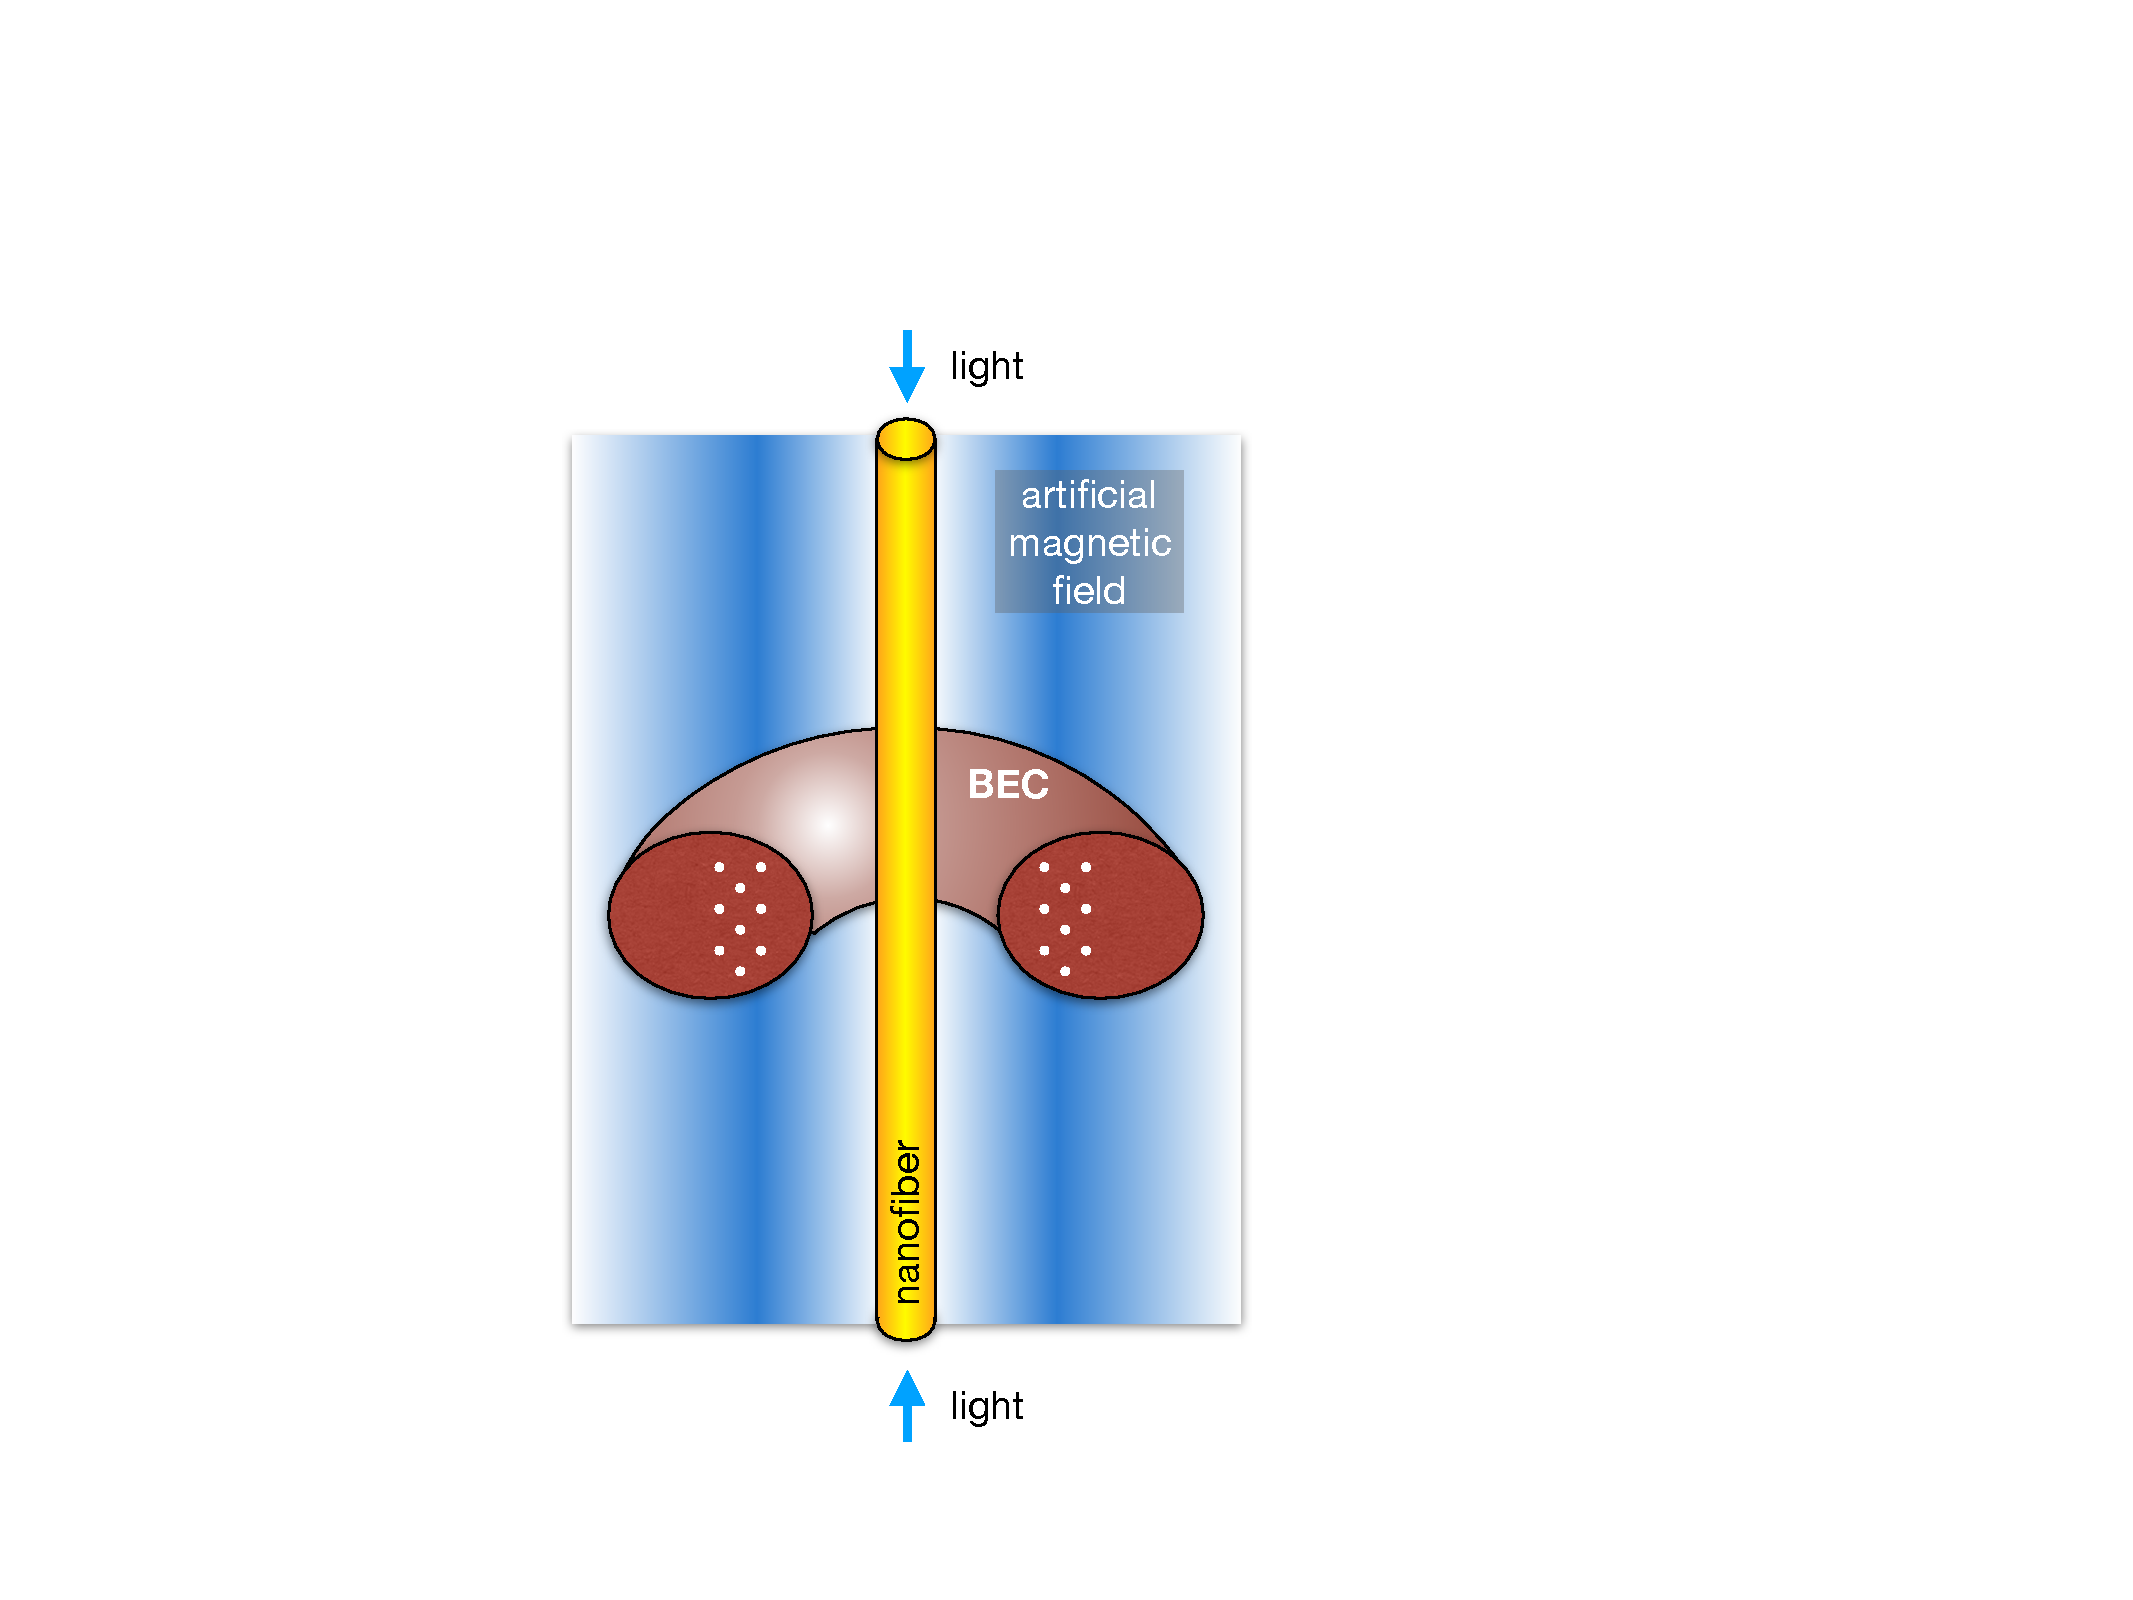
\includegraphics[width=0.4\textwidth]{data/3d/Schematic_TB}
\end{center}
\caption{Schematic of the system. Blue or red-detuned light is sent into the nanofiber (yellow), creating an evanescent field and artificial magnetic field (blue) that influences the BEC (maroon) held by a toroidal trapping potential. If the artificial magnetic field strength is greater than a threshold value, vortex rings (white) will appear and begin to arrange themselves into a triangular lattice.}
\label{fig:device}
\end{figure}

With this same device, it is also possible to detect whether a vortex ring is present in the system by exciting the scissors mode in an elliptic-toroidal trapping geometry~\cite{cozzini2003, guery1999, marago2000}.
This can be done by tilting the trap radially from the center of the torus, which will cause the BEC to oscillate in and out in the new potential, similar to the oscillation shown in Chapter~\ref{ch:splitop} for a simple harmonic oscillator.
Without a vortex present, this oscillation possesses a single frequency, whereas in the presence of a vortex ring, it will contain two frequencies that average to the vortex-less oscillation frequency, similar to scissors mode oscillations in a two-dimensional, elliptically-trapped BEC~\cite{smith2004, zambelli1998, stringari2001}.

\subsection{Bose--Einstein condensate dynamics in the presence of an optical nanofiber}

As discussed in Chapter~\ref{ch:splitop}, in the presence of an artificial magnetic field, the GPE becomes,

\begin{equation}
i\hbar \frac{\partial \Psi}{\partial t} = \left[\frac{(p-m\mathbf{A}({\bf r}))^2}{2m} + V_{\text{trap}}({\bf r}) + g|\Psi|^2 \right] \Psi.
\end{equation}

\noindent Here, all values are defined as before.
The artificial vector potential can take many forms, but for here, I will again choose a description based on Berry's connection~\cite{dalibard2011},

\begin{equation}
  \mathbf{A} = i\hbar \braket{\Psi_l | \nabla \Psi_l},
\end{equation}
\noindent where $\Psi_l$ is the atomic wavefunction in some dressed state $l$.

Considering a dressed, two-state atoms in the presence of an optical field, these states can be written within the rotating wave approximation as~\cite{mochol2015},
\begin{align}
\ket{\Psi_1({\bf r})} &= 
\begin{pmatrix}
    \cos[\Phi({\bf r})/2] \\
     \sin[\Phi({\bf r}) /2]e^{i\phi(z)} 
\end{pmatrix},\\
\ket{\Psi_2({\bf r})} &= 
\begin{pmatrix}
    -\sin[\Phi({\bf r}) /2]e^{-i\phi(z)} \\
    \quad\cos[\Phi({\bf r})/2]
\end{pmatrix},
\end{align}
\noindent where $\phi(z)$ is the phase of the optical field and $\Phi({\bf r}) = \arctan(|\kappa({\bf r})|/\Delta)$, with $\Delta = \omega_0 - \omega$ being the detuning and $\kappa({\bf r}) = \mathbf{d} \cdot \mathbf{E}({\bf r}) / \hbar$ being the Rabi frequency.
The atomic dipole moment is given by $\mathbf{d}$ and $\mathbf{E(\mathbf{r})}$ is the electric field.
Here the form of $\mathbf{A}$ follows the form of the optical fields, and the artificial magnetic field is given by $\mathbf{B}= \nabla \times \mathbf{A}$; therefore, it is possible to influence the magnetic field and vortex structures generated with this system by modifying the optical profile of the nanofiber.

For optical nanofibers, one can determine which modes will propagate in the system by calculating the $V$-number, with $V = k_0a\sqrt{n_1^2 - n_2^2}$, where $a$ is the fiber radius, $n_1$ is the refractive index of the fiber, $n_2$ is the refractive index of the cladding, and $k_0 = \omega/c$ with $\omega$ being the frequency of the input light beam.
The $V$ number can be easily chosen by modifying the radius of the fiber, and the way in which light propagates through the fiber for each mode is characterized by the modal propagation constant, $\beta$.
In addition, the effective refractive index of the fiber is $n_\text{eff} = \beta / \kappa_0$.
In figure~\ref{fig:mode_plot}, a plot of $n_\text{eff}$ vs $V$ number is shown in (a) and it can be seen that certain modes cannot propagate until certain threshold values are reached.
In (b) and (c), the simulated and experimental images of the fiber output are shown as the LP$_{11}$ group, which is a combination of the HE$_{21\text{even}}$, HE$_{21\text{odd}}$, TE$_{01}$ and the TM$_{01}$ modes.
For the system considered in this chapter, the fiber has been tapered such that the cladding is the vacuum, itself, with $n_2=1$; therefore, higher order modes can only be sustained if $V > V_c \simeq 2.405$.
Below this value, only the fundamental mode can propagate in the system.

\begin{figure}

\center 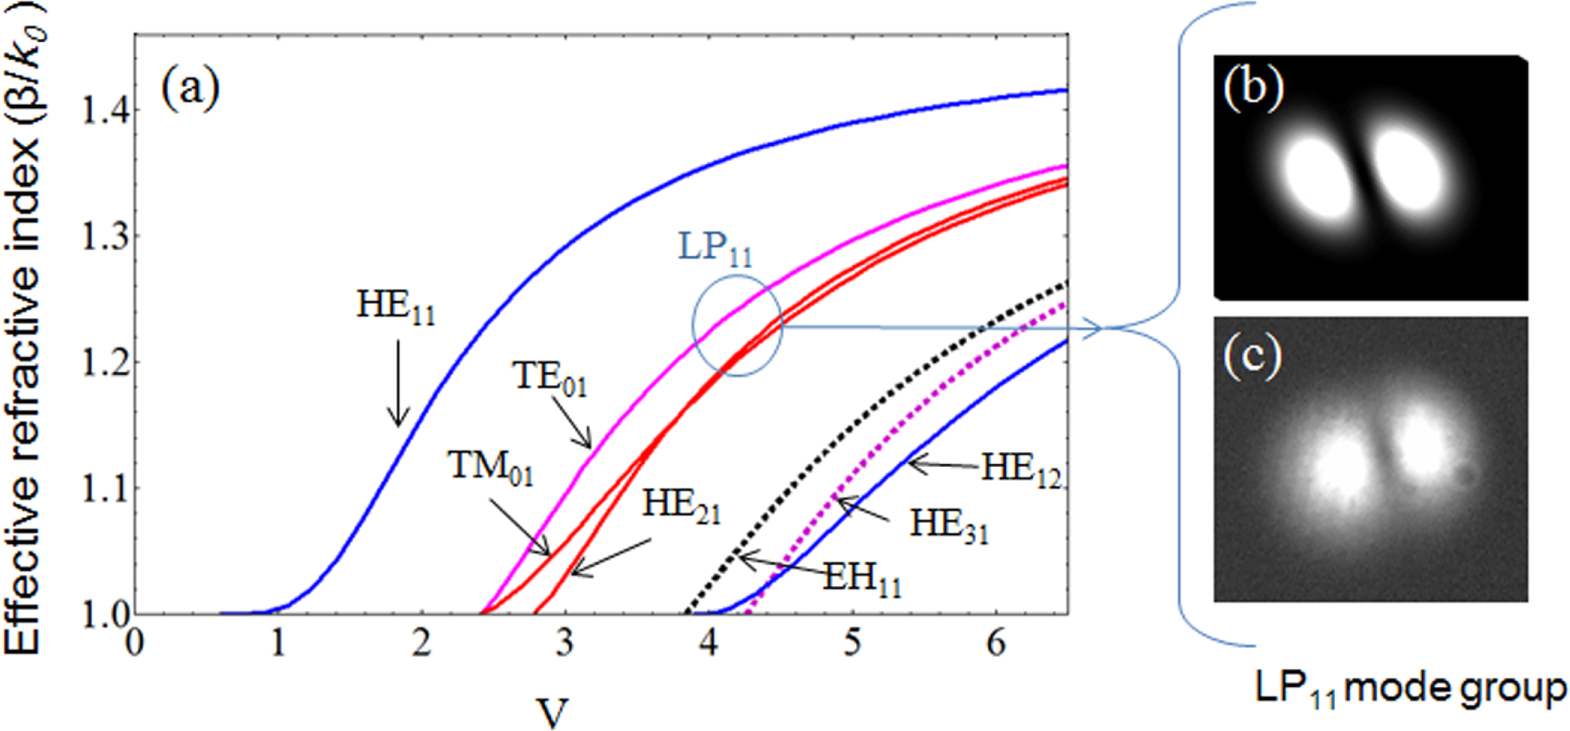
\includegraphics[width=\textwidth]{data/3d/fiber/mode_plot.jpg}
\caption{(a) Plot of effective refractive index and $V$ number of an optical fiber.
The circle indicates the LP$_{11}$ group, which is the first higher-order group composed of the HE$_{21\text{even}}$, HE$_{21\text{odd}}$, TE$_{01}$ and the TM$_{01}$ modes.
(b) Simulated and (c) experimental images of the output from the LP$_{11}$ group are also shown.
Reproduced from ~\cite{nieddu2016, kumar2015}.
}
\label{fig:mode_plot}
\end{figure}

Using cylindrical coordinates, the evanescent field of the HE$_{\ell m}$ mode with circular polarization is~\cite{minogin2010},

\begin{align}
        E_r &= iC[(1-s)K_{\ell-1}(qr) + (1+s)K_{\ell+1}(qr)]e^{i(\omega t- \beta z)}, \\
        E_\phi &= -C[(1-s)K_{\ell-1}(qr) - (1+s)K_{\ell+1}(qr)]e^{i(\omega t- \beta z)}, \\
        E_z &= 2C(q/\beta)K_\ell(qr)e^{i(\omega t - \beta z)},
\end{align}
where
\begin{align}
        s &= \frac{1/h^2a^2 + 1/q^2a^2}{J_\ell'(ha)/[haJ_\ell(ha)]+K_\ell'(qa)/[qaK_\ell(qa)]}, \\
        C &= \frac{\beta}{2q}\frac{J_\ell(ha)/K_\ell(qa)}{\sqrt{2\pi a^2(n_1^2N_1+n_2^2N_2)}},
\end{align}
and 
\begin{align}
N_1 =&\frac{\beta^2}{4h^2}\Big[(1-s)^2\left[J_{\ell-1}^2(ha)+J_\ell^2(ha)\right]\nonumber \\
   & \qquad+(1+s)^2\left[J_{\ell+1}^2(ha)-J_\ell(ha)J_{\ell+2}(ha)\right]\Big] \nonumber\\
   & +\frac12\left[J_\ell^2(ha) - J_{\ell-1}(ha)J_{\ell+1}(ha)\right], \\
N_2 =& \frac{J_\ell^2(ha)}{2K_\ell^2(qa)}\Bigg( \frac{\beta^2}{4q^2}\Big[(1-s)^2\left[K_{\ell-1}^2(qa)-K_\ell^2(qa)\right] \nonumber\\
   & \qquad\qquad\quad-(1+s)^2\left[K_{\ell+1}^2(qa)-K_\ell(qa)K_{\ell+2}(qa)\right]\Big] \nonumber\\
   & \qquad\qquad \left[K_\ell^2(qa) + K_{\ell-1}(qa)K_{\ell+1}(qa)\right]\Bigg ).
\end{align}
The mode geometry is given by $J_n(x)$, the Bessel function of the first kind, $K_n(x)$, the modified Bessel function of the second kind, and $\beta$, the propagation constant of the fiber.
The scaling factors are given by $q = \sqrt{\beta^2-n_2^2k_0^2}$ and $h = \sqrt{n_1^2k_0^2 - \beta^2}$, the normalization constant is $C$ and $s$ is a dimensionless parameter.

\begin{figure}[tb]
 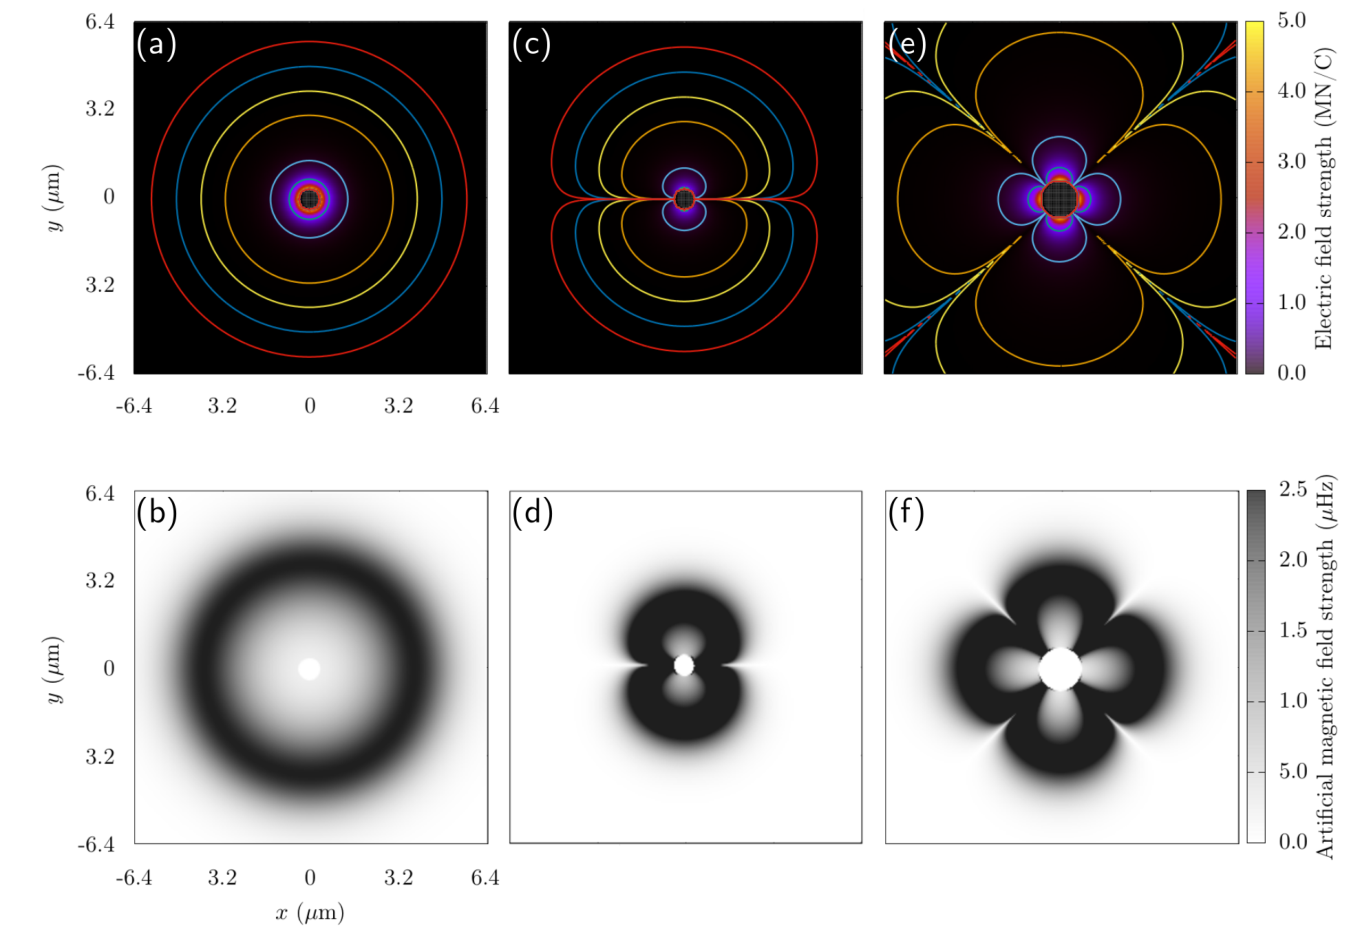
\includegraphics[width=\linewidth]{data/3d/all_fields.pdf}
         \caption{Images of electric and artificial magnetic field profiles for [(a) and (b)] the fundamental HE$_{11}$ mode with circular polarization, [(c) and (d)] the HE$_{11}$ mode with linear polarization, and [(e) and (f)] the HE$_{21}$ mode with linear polarization. For these calculations, the input power is 372~nW in (a) and (b) , 16~nW in (c) and (d), and 418~nW in (e) and (f). For the HE$_{11}$ mode, the nanofiber radius is 200~nm with blue-detuned light of 700~nm, and for the HE$_{21}$ mode, the nanofiber radius is 400~nm with red-detuned light of 980~nm}
 \label{fig:EtoB}
\end{figure}

When the input light field is linearly polarized, it is convenient to write the  Cartesian components of the evanescent electric field as 
\begin{align}
E_x =& \sqrt 2 C\Big[(1-s)K_{\ell-1}(qr)\cos(\phi_0)
      +(1+s)K_{\ell+1}(qr)\cos(2\phi-\phi_0)\Big]e^{i(\omega t - \beta z)}, \\
E_y =&\sqrt 2 C\Big[(1-s)K_{\ell-1}(qr)\sin(\phi_0)
      +(1+s)K_{\ell+1}(qr)\sin(2\phi-\phi_0)\Big]e^{i(\omega t - \beta z)}, \\
E_z = & 2\sqrt 2 i C(q/\beta)K_\ell(qr)\cos(\phi - \phi_0)e^{i(\omega t - \beta z)}.
\end{align}
Here $\phi_0$ determines the orientation of polarization, with $\phi_0 = 0$ being along the $x$ axis and $\pi/2$ being along the $y$ axis.
The artificial vector potential produced by such evanescent fields around an optical nanofiber is then given by \cite{sachdeva2017}
\begin{equation}
\mathbf{A} = \hat{z} \hbar \kappa_0 (n_1 + 1) \tilde{s} \left[\frac{|d_rE_r + d_{\phi}E_{\phi} + d_zE_z|^2}{1 + \tilde s^2|d_rE_r + d_{\phi}E_{\phi} + d_zE_z|^2} \right],
\end{equation}
where $\tilde s = \frac{|\mathbf{d}\cdot\mathbf{E}|}{\hbar |\Delta|}$ and
the corresponding magnetic field $\mathbf{B} = \nabla \times \mathbf{A}$ can be calculated to be
\begin{align}
\mathbf{B} =& \frac{\hbar \kappa_0 s^2(n_1 + 1)}{(1+\tilde s^2|d_rE_r + d_{\phi}E_{\phi} + d_zE_z|^2)^2} \nonumber\\
&\times \bigg[ \hat\phi  \frac{\partial}{\partial r} |d_rE_r + d_{\phi}E_{\phi} + d_zE_z|^2 \nonumber\\
&\qquad- \hat r \frac{1}{r} \frac{\partial}{\partial \phi} |d_rE_r + d_{\phi}E_{\phi} + d_zE_z|^2 \bigg ].
\end{align}
This shows that the $\mathbf{B}$ field has only components in the $\hat \phi$ and $\hat r$ directions, which means that all field lines lie in the horizontal plane if the fiber is aligned along the vertical $\hat z$ direction.

This also means that a BEC trapped toroidally around the nanofiber would facilitate vortex structures that wrap around the nanofiber and potentially close on themselves in the form of vortex rings; however, other vortex structures are possible as well.
In addition, the value of $\tilde s$ governs the amplitude and range of the magnetic field, and as such, it is possible to manipulate the size and shape of the generated vortex rings by changing the detuning and intensity of the electric field~\cite{sachdeva2017}.

For the purposes of this project, I will consider the fundamental HE$_{11}$ mode with circular polarization, the HE$_{11}$ mode with linear polarization, and the HE$_{21}$ mode with linear polarization.
Though even higher-order modes may be generated by the optical nanofiber, increasing the $V$-number to facilitate these modes also requires increasing the fiber radius beyond what is experimentally achievable.
It is also possible to create even more complex field configurations by interfering different modes; however, the chosen modes will still demonstrate a range of possible magnetic field profiles.
The electric field configurations and their corresponding magnetic field profiles can be seen in Figure~\ref{fig:EtoB}.
Here, the circularly polarized HE$_{11}$ mode will create a cyllindrically symmetric electric (a) and magnetic (b) field profiles; however, linearly polarized light will create a lobed structure for both (c and d).
When using the linearly-polarized HE$_{21}$ mode, four petals appear in the electric and magnetic field profiles, which suggest unusual vortex structures.
Now I will discuss what types of vortex structures can be generated with this system, including the possibility of generating vortex ring lattices.

\subsection{Ground state vortex configurations}

\begin{figure}[tb]
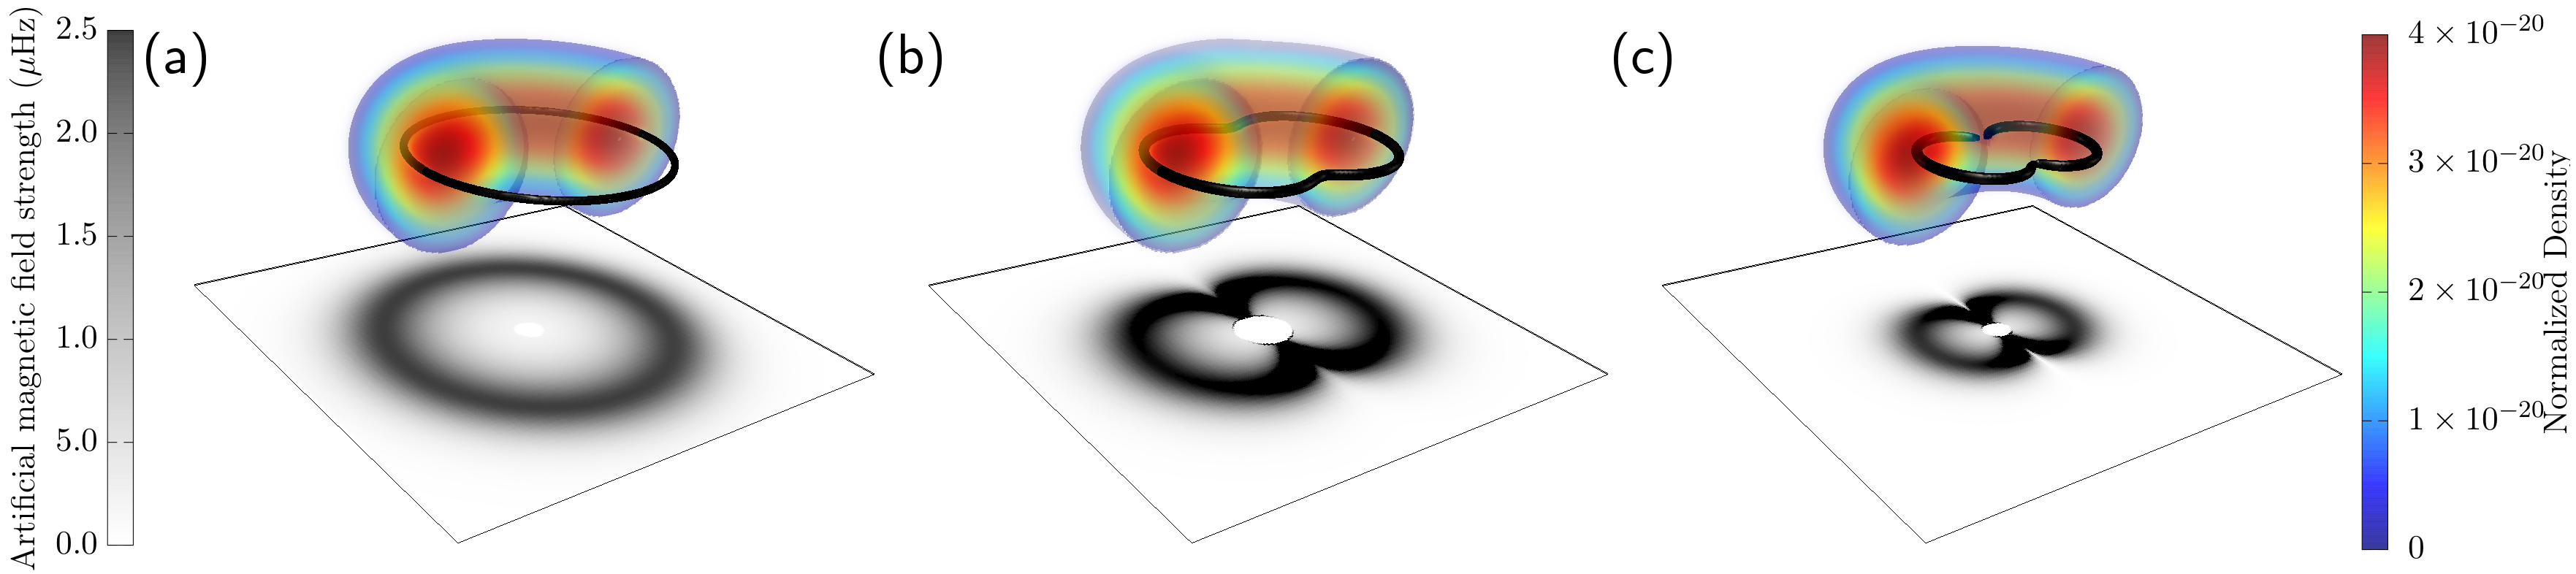
\includegraphics[width=\textwidth]{data/3d/vortex_transition.png}
\caption{Vortex configurations for different magnetic field profiles from the nanofiber for the fundamental HE$_{11}$ mode with (a) circular polarization, (b) elliptical polarization, and (c) linear polarization along the $\hat y$ direction.
The vortex distributions have been found via an isosurface on the Sobel filtered wavefunction density for a $^{87}$Rb BEC and all optical fiber fields are normalized and for a nanofiber of 200~nm in radius with blue-detuned light of 700nm.
The magnetic field profiles shown in the shaded region beneath wavefunction density are similar to those in Figure~\ref{fig:EtoB}(b) and (d).}
\label{fig:VortexRings}
\end{figure}

We will use GPUE~\cite{schloss2018} to describe a $^{87}$Rb condensate with $1\times10^5$ atoms with a scattering length of $a_s=4.76 \times 10^{-9}$ m on a three-dimensional grid of $256^3$ points with a spatial resolution of 50 nm, with a toroidal trapping potential around the fiber given by,
\begin{equation}
V_\text{trap} = m(\omega_r^2(r-\eta)^2 + \omega_z^2z^2),
\label{eqn:potential}
\end{equation}

\noindent where the frequencies in the $\hat r$ and $\hat z$ directions are chosen to be $\omega_r = \omega_z = 7071$Hz to match typical experimental conditions in fiber trapping \cite{vetsch2010}.
Here, $\eta$ describes the distance of the center of the torus from the center of the fiber and is chosen such that the atoms are trapped beyond the van-der-Waals potential of the fiber.
For the HE$_{11}$ mode, the fiber radius is 200\,nm and $\eta = 3.20$\,$\mu$m, creating a toroidal BEC with an inner radius of roughly 300\,nm from the fiber surface.
For the HE$_{21}$ mode, the fiber radius is increased to 400 nm, but keep all other parameters the same, creating a toroidal BEC with an inner radius of roughly 150 nm.

\begin{figure}[tb]
\center 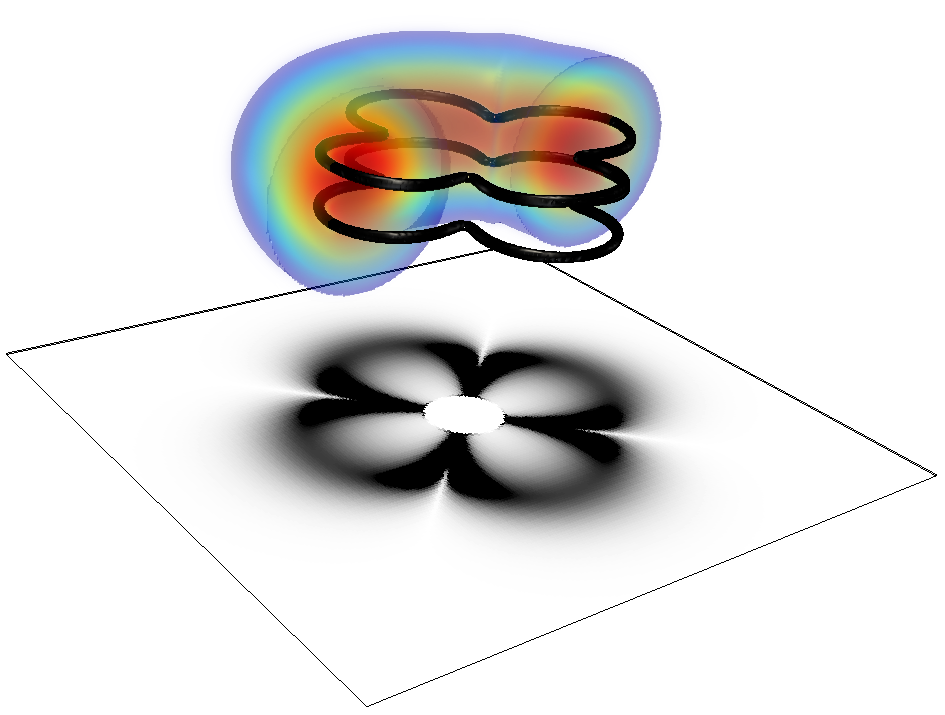
\includegraphics[width=0.5\linewidth]{data/3d/HE21_3d.png}
 
 \caption{Vortex configuration for the HE$_{21}$ mode with linear polarization along the $\hat y$ direction.
\label{eqn:potential}
The magnetic field profile is similar to the one shown in Figure~\ref{fig:EtoB}(f), and has been calculated for a nanofiber of 400~nm in radius with red-detuned light of 980~nm.}
 \label{fig:HE21_3d}
\end{figure}

As shown in Figure~\ref{fig:VortexRings}(a), when simulating the HE$_{11}$ mode with these parameters, one can see a vortex line that wraps around the fiber and reconnect in the form of a single vortex ring as the ground state solution.
In contrast, the linearly polarized HE$_{11}$ mode in Figure~\ref{fig:VortexRings}(c) shows a ground state where the vortex lines bend toward the center of the torus, creating two vortex lobes.
As a note, the vortex lines do not follow the magnetic field lines exactly, but instead reconnect to the neighboring lobe when approaching each other within a healing length.
If elliptically polarized light is considered, one can see a hybrid ground state between the circularly and linearly polarized modes, shown in Figure~\ref{fig:VortexRings}(b).
Finally, I show a four-petal ground-state solution when using the HE$_{21}$ linearly polarized mode in Figure~\ref{fig:HE21_3d}.
Here, I also show that it is possible to generate multiple vortex structures in-line with themselves by increasing the intensity of the artificial magnetic field.

\begin{figure}
\center 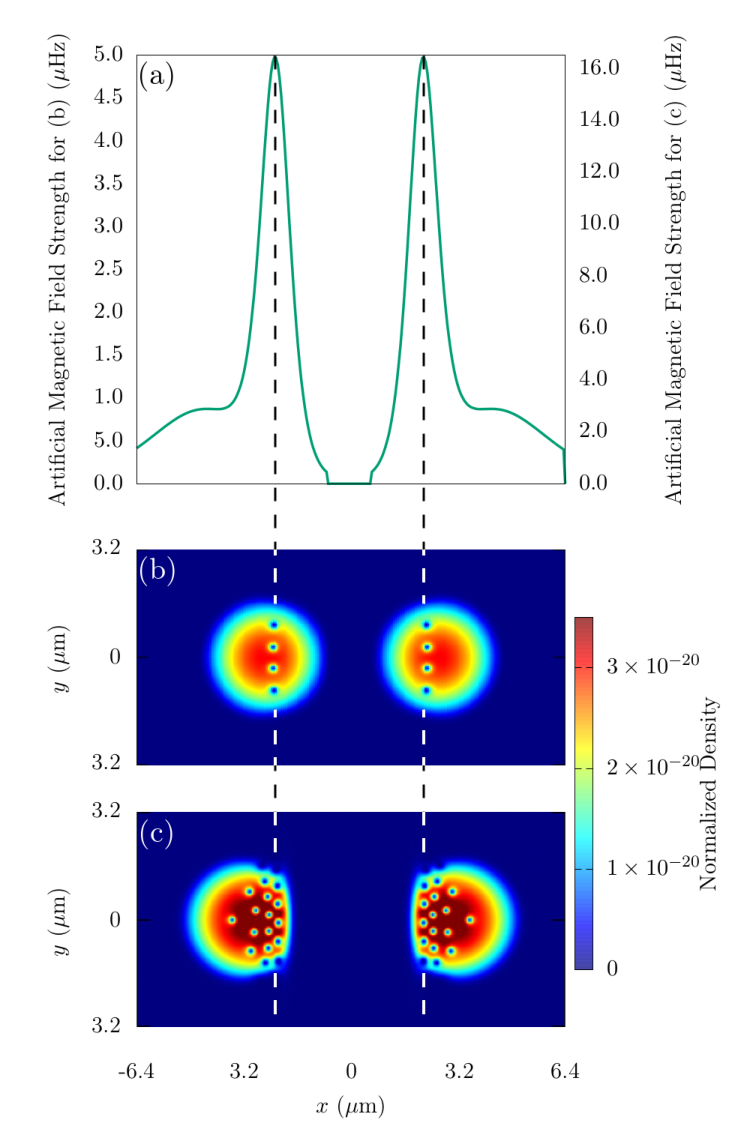
\includegraphics[width=0.8\linewidth]{data/3d/vortex_line_all.pdf}
\caption{(a) The magnetic field profile along the $x$-direction for the fundamental HE$_{11}$ mode with circular polarization outside a fiber of 200~nm radius.
Note that for this mode and polarization the whole system is azimuthally symmetric.
For weak fields (see (b)) this leads to a small number of vortices that align along the line at which the magnetic field is maximal and for larger fields (see (c)) more vortex rings appear that form the beginning of an Abrikosov lattice.
The optical fiber field and wavefunction density have been normalized and are for a nanofiber of 200~nm in diameter with blue-detuned light of 700nm and a $^{87}$Rb BEC respectively.}
\label{fig:field_triangular}
\end{figure}

This indicates that it is possible to generate interesting vortex ring lattice structures in three-dimensions by sufficiently increasing the artificial magnetic field.
To study the control of multiple vortex structures with this system, I first simulated a system with low artificial magnetic field strength and showed that this simulation will cause all vortex rings to line up at peaks in the magnetic field in Figure~\ref{fig:field_triangular}(a and b).
As the magnetic field is increased from this point, the vortex rings begin to pack together and form an Abrikosov-like lattice in-line with peaks in the artificial magnetic field, shown in Figure~\ref{fig:field_triangular}(a and c).
If other magnetic field profiles are used, it could be possible to generate different Abrikosov-like ring lattice configurations.
This system could allow for studies of bulk vortex-ring movement, thereby potentially creating a vortex ring lattice that rotates in a leapfrogging manner and moves based on individual vortices self-induced velocity.

The optical nanofiber seems to provide unprecedented control over the vortex geometries generated in a toroidally-trapped BEC system, and one can control the shape of each vortex structure by manipulating the optical fields input into the nanofiber.
In addition, because the optical fields could be time-dependent, this system could be used in the future to probe dynamical effects of vortices.
In this case, one must consider the effects of high artificial magnetic fields on the distribution of atoms, themselves, because (as described in Chapter~\ref{ch:splitop}), the external potential $V_\text{trap}$ will be modified by a term proportional to $\mathbf{A}^2$.
In Figure~\ref{fig:V_change}, I show this modification for the artificial magnetic fields shown in Figure~\ref{fig:field_triangular}(c).
Dynamical studies in which the gauge field is switched off in a finite time will thus lead to phonon excitations in the condensate, which will also influence the vortex lines, themselves, and this is an area of future work.

\begin{figure}
\center 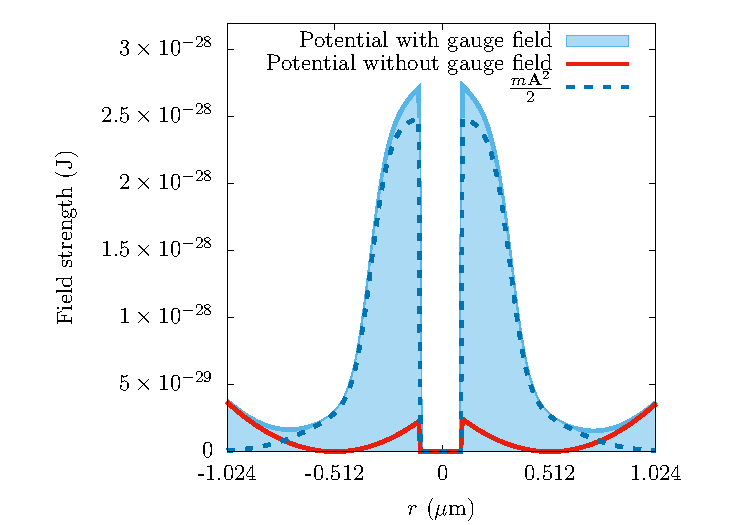
\includegraphics[width=0.75\textwidth]{data/3d/V_change.pdf}
\caption{Visualization of the change in potential due to the effects of the artificial magnetic field for Figure~\ref{fig:field_triangular}.
Here, the experienced potential is shown in the blue shaded region, the scaled artificial vector potential is shown as a dotted, dark blue line, and the original trap is shown in red.}
\label{fig:V_change}
\end{figure}

\subsection{Dynamic vortex detection and scissor modes}

\begin{figure}
\center 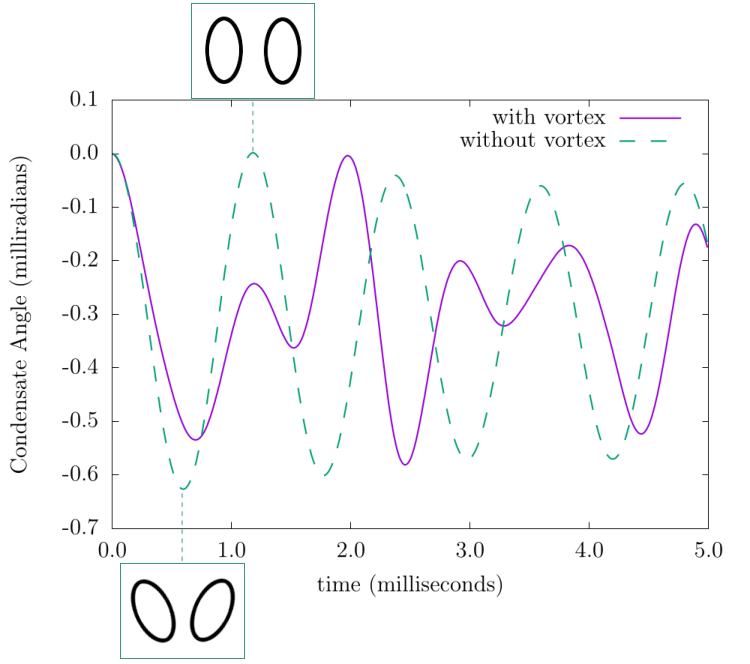
\includegraphics[width=0.75\textwidth]{data/3d/scissors_plot.pdf}
\label{fig:scissors}
\caption{\label{fig:scissors} Angle of the condensate axis after excitation of the toroidal scissors mode for an elliptic-toroidal BEC with a single vortex ring (purple, solid) and without a vortex present (cyan, dashed).
Depictions of two dimensional slices for the scissors mode without a vortex are shown in the insets.
Here, the scissors mode causes oscillation in and out towards the center of the system, and that two distinct frequencies are present in the curve for the condensate carrying a vortex ring. }
\end{figure}

Observing the presence of vortex rings in a three dimensional BEC is a difficult problem, as absorption spectroscopy usually only provides a picture of an integrated two-dimensional density.
However, due to the unique geometry of this system, one can identify whether vortex rings are present by exciting the scissors mode of the condensate \cite{cozzini2003, guery1999, marago2000}. 
For an elliptic-toroidal geometry ($\omega_z < \omega_r$), the scissors mode can be excited by modifying the external potential with a rotation in the $rz$-plane,
\begin{equation}
        V = V_{\text{trap}}(r, \theta, z) -m\omega_0^2\alpha rz,
\end{equation}
where $\alpha = 2\epsilon\theta$ is a coefficient related to the tilting angle, $\epsilon$ is the deformation of the trap in the $rz$ plane and $\theta$ is the angle at which the original trap was aligned at.
For a small initial angle of $\theta_0$ this change in the potential causes a BEC without rotation to oscillate back and forth in the trap with a frequency given by \cite{stringari2001}
\begin{equation}
        \omega_{\text{scissors}} = \sqrt{\omega_r^2+\omega_z^2}.
\end{equation}
If, however, this mode is excited for a BEC that contains a vortex line, the oscillation will be strongly influenced by the currents inside the condensate and two different frequencies ($\omega_+$ and $\omega_-$) appear in the oscillation~\cite{smith2004, zambelli1998, stringari2001}.
When the splitting frequency is small compared to the scissors mode frequency, it 
can be written as \cite{zambelli1998}
\begin{equation}
\omega_{+} - \omega_{-} = \frac{\langle l_z \rangle}{m\langle r^2 + z^2 \rangle},
\label{eqn:splitting}
\end{equation}
where $\langle l_z \rangle$ is the average angular momentum per particle.
Calculating these values for the system for $\omega_r = 4242$Hz, and $\omega_z = 2828$Hz then leads to $\omega_{\text{scissors}} = 5090$Hz, $\omega_{-} = 3765$Hz, and $\omega_{+} = 6415$Hz, which are very close to the values observed in the numerical simulations shown in Fig.~\ref{fig:scissors}.
However, one can also see from this figure that the oscillation is not perfect and seems to decay over time.
This is due to the above mentioned modification of the trapping potential by the artificial vector potential, which leads to a deviation from the perfect elliptical toroidal shape used in the derivation of Equation~\eqref{eqn:splitting}.

It is worth noting that this method cannot be used to detect a vortex ring inside a simply connected condensate, as in this situation the flow around the vortex line has no preferred direction.
However, in the toroidal shape, each radial slice can be seen as a two-dimensional elliptical BEC with a single vortex, and the system will therefore exhibit the scissors mode frequency as expected.
While in principle the excitation of the scissors mode can also be used to detect Abrikosov vortex-ring lattice, the fact that the inhomogeneous artificial magnetic field leads to an inhomogeneous vortex ring distribution will have an effect on the expected oscillation frequencies.

\section{Conclusion}

In this application of the GPUE codebase, I have shown that it is possible to create and control vortex rings and more complicated vortex structures by using the artificial magnetic field generated by the optical nanofiber.
There is currently no other known method to generate the structures created by the linearly polarized modes, shown in Figure~\ref{fig:VortexRings}(b,c) and \ref{fig:HE21_3d}.
We have also shown that the scissors mode can be used to detect whether a vortex ring is present in an elliptic toroidal trap.
These fiber-generated structures could allow for experimental systems to study complicated superfluid mechanisms, like the kelvin-mode cascade, superfluid turbulence, or reconnection events between superfluid vortex lines.
These structures might also be the first step in creating knotted vortex lines around an optical nanofiber; however, to generate these structures, the magnetic field must have a dependence on $\hat z$, which is not present in this model.

This project leaves several open fields of study for future work and future simulations with GPUE, including the study of dynamic field effects on vortex structures, the generation of vortex knots in superfluid systems with this device, and studies of vortex ring lattice movement in BEC systems.
For both of these cases, significant work must be performed both theoretically and computationally.

To generate vortex knots with this system, a magnetic field with $\hat z$ must be created.
Such fields might be possible with fiber Bragg gratings~\cite{hill1997} or other methods to change the evanescent profile of the fiber.
Such simulations would require FEM or FDTD simulations of the optical fiber, itself, which makes the problem an intricate engineering process of generating the right field with an optical nanofiber.
In addition, a z-dependent gauge field requires analysis of the other gauge field term, $\frac{p_z\mathbf{A}_z}{2}$, which is not considered in this work because the derivative along the $\hat z$ direction for the fiber field is 0.
This leads to interesting questions about how BEC systems behave in the presence of such artificial magnetic fields.

For the movement of dynamic vortex ring tangles generated with this system, vortex tracking methods in three-dimensions should be employed.
As described in Chapter~\ref{ch:gpu}, this is not a trivial task and I will discuss methods that could be used to do this in the Conclusion~\ref{ch:conclusion}.
It is also interesting to see what happens if the HE$_{21}$ vortex structures are evolved in real-time and whether scissors modes can be used to detect such vortex structures as well.
With a sharp magnetic field, it is also possible to create a phase separation along a vortex line for multicomponent condensate simulations.


\unnumberedchapter{Conclusion} % Title of the unnumbered chapter
\chapter*{Conclusion}

\section{Overall conclusions}

\label{ch:conclusion}

This thesis has presented my efforts to create a massively parallel SSFM codebase for the simulation of superfluid vortex dynamics in Bose--Einstein Condensates (BECs).
Starting from the SSFM and a discussion on the dynamics of ultracold atomic systems, I motivated the dynamic quantum engineering by introducing quantum optimal control and shortcuts to adiabaticity.
Both of these methods were used to show that it is possible to generate macroscopic superposition states in a Tonks--Girardeau gas when on a ring with a barrier to break rotational symmetry.
From there, I introduced the GPGPU and the GPUE codebase, emphasizing existing challenges in the field and the methods I used to overcome them.
In the process, I also briefly mentioned the challenging problem of memory coaliescence when using spectral methods on GPU hardware and proposed an additional software package as method to further optimize the FFT operations with a distributed, multi-GPU transpose.
After this, I introduced an example physical system that showed it is possible to generate chaotic vortex dynamics in few-vortex systems and emphasized the need for vortex tracking methods and post-processing methods, by calculating the Lyapunov exponent on the vortex trajectories.
Finally, I introduced a three-dimensional example system that generates, controls, and detects vortex ring-like geometries in a toroidally-trapped BEC coupled to the artificial magnetic field generated by an optical nanofiber.

Throughout this work, there are several physical and computational areas that require further development in the future and these will be further discussed in this section.

\jrs{Not really sure which future directions to highlight here...}
\section{Further development of GPUE}

Though the GPUE codebase is roughly feature complete, there are several directions for future development, many of which were described in Chapter~\ref{ch:gpu}.
In particular, a re-write of GPUE in julia along with developing an $n$-dimensional, distributed, GPU transpose are currently being worked on.
The former will allow for GPUE to be more maintainable and require less development time in the future.
The latter is applicable to a wide range of spectral methods and might allow for several methods to become relevant again on HPC environment.
As both of these were discussed at length in Chapter~\ref{ch:gpu}, I will not discuss them further here; however,
there are future directions where proper development has not begun, such as new vortex tracking methods and potentially using expression trees for general-purpose Hamiltonian solutions.

\subsection{Vortex tracking in $n$ dimensions}

The GPUE codebase currently has the capability of tracking vortices in two dimensions and highlighting vortices in three; however, vortex tracking has yet to be implemented as there are no reliable and general methods for tracking three dimensional vortex structures in superfluid simulations.
In addition, the vortex tracking method in GPUE is currently unstable for non-harmonic traps in two dimensions, and in many cases, the user does not know the precise geometry of the trapping system.
As such, a generalized vortex tracking methods for $n$-dimensional simulations is desired.

In 2016, a method for three dimensional vortex tracking was proposed by Villois \textit{et. al.}~\cite{villois2016}; however, this method has no computational complexity bound, assumes periodic boundary conditions, and required a large amount of communication between the device and host.
We have considered development of a similar method that leverages our vortex highlighting scheme to create $n$-dimensional vortex skeletons for vortex tracking in two and three dimensions.
\jrs{ADD MORE IF KEEPING}

\subsection{General purpose Hamiltonian solver}

\subsubsection{GPUE.jl}
After considering our options, we have begun development of GPUE.jl, the a julia re-write of GPUE.

\section{Future simulations of quantum systems}

In addition to further developments of GPUE, there are also several new simulations that can be performed now on GPU hardware, such are multicomponent simulations with gauge fields and dynamic studies of the system introduced in Chapter~\ref{ch:vortex_states}.
Because GPUE allows for the simulation of dynamic variables through expression trees, further three-dimensional STA studies can also be performed.

Ultimately, this work has provided a toolbox for the simulation of various quantum phenomenon that were computational inctractable before now, including the three-dimensional simulations of superfluid turbulence without relying on vortex-filament mthods, and simulations of multicomponent systems with gauge fields.
It has also developed novel methods for maximizing the size of the simulated domain with the SSFM, along with tools like the DistributedTranspose.jl that allow for spectral methods to be more widely used in HPC environments.
 % Conclusion (unnumbered)

%-------------------------------------------------------------------------------
%	APPENDICES
%-------------------------------------------------------------------------------
\addtocontents{toc}{\vspace{2em}} % Add a gap in the Contents, for aesthetics
\appendix

\numberedchapter % Regular chapters following
\input{MainText/appendixGPU}
%\input{MainText/appendixB}
%\input{MainText/appendixC}

%-------------------------------------------------------------------------------
%	BIBLIOGRAPHY
%-------------------------------------------------------------------------------

\addtocontents{toc}{\vspace{2em}} % Add a gap in the Contents, for aesthetics
\unnumberedchapter{Bibliography} % Title of the unnumbered chapter
\bibliography{Preamble/Thesis_bibliography} % The references information are stored in the file named "Thesis_bibliography.bib"


\end{document}
